%Tipo de documento
\documentclass[12pt,letterpaper]{article}
%Preámbulo
\usepackage[utf8]{inputenc} %Codificación
\usepackage[spanish]{babel}
\usepackage{blindtext}
\usepackage{courier}
\usepackage{xcolor}
\usepackage{graphicx}
\usepackage{multicol}
\usepackage{float}
\usepackage{fancyhdr}
\usepackage{tikz}
\usepackage{mathptmx} %Times new roman
\usetikzlibrary{babel}
\usepackage{amsmath, amssymb, latexsym}
\numberwithin{equation}{section}
\usepackage[letterpaper]{geometry}
% Paquete geometry tamaño carta
\geometry{verbose,tmargin=3cm,bmargin=2.5cm,lmargin=3cm,rmargin=2cm}
% Configuración de márgenes
\setlength{\columnsep}{1cm}
\setlength{\columnseprule}{2pt}
%Inclusión de códigos
%%%%%%%%%%%%%%%%%%%%%%%%%%%%%%%%%%%%%%%%%%%%%%%%%%%%%%%%%
%%%%%%%%%%%%%%%%%%%%%%%%%%%%%%%%%%%%%%%%%%%%%%%%%%%%%%%%%
\usepackage{listings}

\definecolor{myblue}{rgb}{.26, .44, .56}
\definecolor{mygreen}{rgb}{.12,.54,.11}
\definecolor{mygray}{rgb}{0.5,0.5,0.5}
\definecolor{mymauve}{rgb}{.6,0,0}
\definecolor{mypink}{rgb}{.698,.145,.698}

\lstset{ %
	backgroundcolor=\color{white},   % choose the background color; you must add \usepackage{color} or \usepackage{xcolor}
	basicstyle=\footnotesize,        % the size of the fonts that are used for the code
	breakatwhitespace=false,         % sets if automatic breaks should only happen at whitespace
	breaklines=true,                 % sets automatic line breaking
	captionpos=b,                    % sets the caption-position to bottom
	commentstyle=\color{myblue},    % comment style
	deletekeywords={...},            % if you want to delete keywords from the given language
	escapeinside={\%*}{*)},          % if you want to add LaTeX within your code
	extendedchars=true,              % lets you use non-ASCII characters; for 8-bits encodings only, does not work with UTF-8
	frame=single,	                   % adds a frame around the code
	keepspaces=true,                 % keeps spaces in text, useful for keeping indentation of code (possibly needs columns=flexible)
	%classoffset=0, 
	keywordstyle=\color{mygreen},       % keyword style
	%classoffset=1, %morekeywords={*,<,==,!=,>,/},keywordstyle=\color{mypink},
	%classoffset=0,
	language=Python,                 % the language of the code
	otherkeywords={...},           % if you want to add more keywords to the set
	numbers=left,                    % where to put the line-numbers; possible values are (none, left, right)
	numbersep=5pt,                   % how far the line-numbers are from the code
	numberstyle=\tiny\color{mygray}, % the style that is used for the line-numbers
	rulecolor=\color{black},         % if not set, the frame-color may be changed on line-breaks within not-black text (e.g. comments (green here))
	showspaces=false,                % show spaces everywhere adding particular underscores; it overrides 'showstringspaces'
	showstringspaces=false,          % underline spaces within strings only
	showtabs=false,                  % show tabs within strings adding particular underscores
	stepnumber=2,                    % the step between two line-numbers. If it's 1, each line will be numbered
	stringstyle=\color{mymauve},     % string literal style
	tabsize=2,	                   % sets default tabsize to 2 spaces
	title=\lstname                   % show the filename of files included with \lstinputlisting; also try caption instead of title
}



%%%%%%%%%%%%%%%%%%%%%%%%%%%%%%%%%%%%%%%%%%%%%%%%%%%%%%%%%
%%%%%%%%%%%%%%%%%%%%%%%%%%%%%%%%%%%%%%%%%%%%%%%%%%%%%%%%%
\title{Tesis}
\author{Milan Ungerer Muñoz}
\date{\today}
%Documento
\begin{document}
%Portada	
\begin{titlepage}
	
	\begin{center}
		\vspace*{-1in}
		
		\Large \textbf{UNIVERSIDAD TÉCNICA FEDERICO SANTA MARÍA}\\
		\vspace*{0.15in}
		\large \textbf{DEPARTAMENTO DE INGENIERÍA MECÁNICA} \\
		\vspace*{0.15in}
		\textbf{VALPARAÍSO - CHILE}
		
		\begin{figure}[h!]
			\centering\includegraphics[height=50mm]{Imagenes/Logo_UTFSM.png}
		\end{figure}
		\vspace*{0.15in}
		\Large \textbf{ESTUDIO NUMÉRICO-COMPUTACIONAL DE LA DISPOSICIÓN IDEAL DE MICROHILOS FERROMAGNÉTICOS EN UN DISPOSITIVO SENSOR DE TENSIONES EN POLÍMEROS}\\
		\vspace*{1in}
		\large\centering \textbf{MILAN SIMÓN ENRIQUE UNGERER MUÑOZ}\\
		\vspace*{0.15in}
		\centering\normalsize \textbf{MEMORIA DE TITULACIÓN PARA OPTAR AL TÍTULO DE INGENIERO CIVIL MECÁNICO MENCIÓN ENERGÍA}\\
		\vspace*{0.6in}
		\centering\normalsize \textbf{PROFESOR GUÍA: \hspace{2.5cm} CHRISTOPHER COOPER VILLAGRÁN}\\
		\vspace*{0.15in}
		\centering\normalsize \textbf{PROFESOR CORREFERENTE: \hspace{1cm} ALEJANDRO PACHECO SANJUAN}\\
		\vspace*{1in}
		\centering\normalsize \textbf{ABRIL - 2017}\\
	\end{center}
	
\end{titlepage}
%%%%%%%%%%%%%%%%%%%%%%%%%%%%%%%%%%%%%%%%%%%%%%%%%%%%%%%%%%%
%%%%%%%%%%%%%%%%%%%%%%%%%%%%%%%%%%%%%%%%%%%%%%%%%%%%%%%%%%%
%Resumen
\pagenumbering{gobble}% Remove page numbers (and reset to 1)
\newpage\null\thispagestyle{empty}\newpage

\begin{center}
	\section*{Agradecimientos}

	Deseo agradecer en este trabajo, en primer lugar, a mi familia por siempre darme su apoyo en todas mis decisiones. A mis amigos que comparten conmigo esta gran etapa de mi vida llamada juventud. Finalmente, pero no menos importante, al profesor Christopher Cooper y Felipe Rossi por ser un apoyo constante en la realización de este trabajo que ha aportado en gran parte a mi desarrollo profesional.

\end{center}


%%%%%%%%%%%%%%%%%%%%%%%%%%%%%%%%%%%%%%%%%%%%%%%%%%%%%%%%%%%
\pagebreak
\section*{Resumen}
En el último tiempo materiales del tipo compósito han sido sujeto de múltiples estudios debido a la utilidad que presentan sus propiedades especiales. En este trabajo el estudio se orientó a un material compuesto por una matriz dieléctrica con inclusiones de materiales conductores llamados micro-hilos ferromagnéticos. Estos hilos presentan la particularidad de cambiar sus propiedades electromagnéticas frente a un estimulo externo. Al aplicar un campo magnético o una tensión mecánica, la permitividad y permeabilidad del hilo cambian, cambiando así la forma en que se dispersa la radiación electromagnética incidente.

Este trabajo está orientado a encontrar la configuración óptima de los micro-hilos para maximizar el cambio de señal recibida con la finalidad de diseñar un sensor de esfuerzos para materiales dieléctricos. La radiación será del tipo microondas y un estimulo de tensión será simulado. Para alcanzar los objetivos planteados se desarrolló un programa que permite calcular el campo electromagnético dispersado por el compósito en cualquier punto en que se desee posicionar la antena.

Para el cálculo del campo se utilizó la ecuación de Helmholtz por medio de su formulación integral de borde lo que permite una manipulación mas simple al momento de calcular el campo y realizar la interacción entre los diferentes obstáculos. Debido a que esta ecuación no posee una solución analítica es necesario aproximarla por medio de algún método numérico, en este trabajo se utilizó el método de elementos de borde a través de, la librería para Python, BEM++.

La configuración óptima es estudiada bajo 3 experimentos, el primero corresponde a variar la distancia de los hilos en una formación del tipo pantalla. Otra alternativa es estudiar como cambia la señal recibida en función del número de filas de hilos en la matriz. finalmente se estudia el cambio de la composición volumétrica de hilos en el compósito.

Para el caso de una configuración de pantalla se puede apreciar que existe un máximo de cambio de señal de 14.84 \% cuando los hilos se encuentran a 1.6[mm] de espaciamiento. Además, se puede observar que para el caso del estudio del porcentaje volumétrico existe un máximo cuando se tienen 6 hilos alcanzando un cambio de alrededor 4.28\%. Para el caso de añadir más filas no se ven cambios considerables ni bibliografía al respecto. La recomendación es de utilizar 6 hilos con un distanciamiento de 1.6 [mm].\\

\noindent\textbf{Palabras claves:} Método de Elementos de Borde, BEM, BEM++, Micro-hilos, Sensor,\\ Dispersión Múltiple.
%%%%%%%%%%%%%%%%%%%%%%%%%%%%%%%%%%%%%%%%%%%%%%%%%%%%%%%%%%%
\pagebreak
\section*{Abstract}
In the last time composite materials have been subject of multiple studies due to the great utility of the special properties that they present. In this work the study was oriented to a material composed of a dielectric matrix with inclusions of conductive materials called ferromagnetic micro-wires. These wires present the peculiarity of changing their electromagnetic properties in front of an external stimulus. When applying a magnetic field or a mechanical tension the permittivity and permeability change, thus changing the way in which the incident electromagnetic radiation is scattered.

This work is oriented to find the optimal configuration of the micro-wires to maximize the change of signal in order to design a stress sensor for dielectrics. The radiation will be of the microwave type and a mechanic tension stimulus will be used. In order to reach the proposed objectives a program was developed that allows to calculate the electromagnetic field scattered by the composite at any point in which it is desired to position the antenna.

For the calculation of the field the Helmholtz equation was used through its boundary integral formulation which allows a simpler manipulation for the calculate of the field and to realize the interaction between the different obstacles. Because this equation does not have an analytical solution it is necessary to approximate it by means of some numerical method, in this work we used the Boundary Element Method with, the library for Python, BEM ++.

The optimal configuration is studied under 3 experiments, the first one corresponds to varying the distance of the wires in a formation of the type screen. Another alternative is to study how the received signal changes as a function of the number of rows of microwires in the array. Finally the change in the volumetric composition of wires in the composite is studied.

In the case of a screen configuration it can be seen that exist a maximum signal change of 14.84 \% when the wires are at 1.6 [mm] spacing. In addition, it can be observed that for the case of the study of the volumetric percentage there is a maximum when there are 6 wires reaching a change of around 4.28 \%. For the case of adding more rows, we don't see any significant changes or bibliography in this regard. The recommendation is to use 6 wires with a spacing of 1.6 [mm].\\

\noindent\textbf{Keywords:} Boundary Element Method, BEM, BEM++, Micro-wires, Sensor,\\ Multiple Scattering.
%%%%%%%%%%%%%%%%%%%%%%%%%%%%%%%%%%%%%%%%%%%%%%%%%%%%%%%%%%%
\pagebreak
\section*{Glosario}
\begin{itemize}
	\renewcommand\labelitemi{--}
	\item \textbf{Dispersión electromagnética:} proceso en que una onda electromagnética incidente se desvía de su trayectoria a causa de pasar por una no uniformidad. Principalmente se distinguen los procesos de reflexión y refracción. 
	\item \textbf{Número de onda:} se puede definir como el número de ondas que existen en una determinada distancia. Frecuencia espacial.
	\item \textbf{Índice de refracción:} número adimensional que describe cómo se propaga una onda electromagnética en un medio.
	\item \textbf{Material dieléctrico:} material que exhibe polarización frente un campo eléctrico. 
	\item \textbf{Material conductor:} material que permite fluir sus electrones frente a un campo eléctrico. La capacidad de fluir libremente depende de la resistencia y conductividad del material.
	\item \textbf{Microondas:} forma de radiación electromagnética con longitudes de onda desde 1[m] a 1[mm], o con frecuencias desde los 300[MHz] hasta los 30[GHz].
	\item \textbf{Permitividad:} medida de resistencia encontrada cuando se forma un campo eléctrico en un medio.
	\item \textbf{Permeabilidad (magnética):} medida de la capacidad de un material para formar un campo magnético en él.
	\item \textbf{Permitividad relativa:} representación de la permitividad de un medio como un cociente de la permitividad absoluta y la permitividad del vacío. 
	\item \textbf{Permeabilidad relativa:} representación de la permeabilidad de un medio como un cociente de la permeabilidad absoluta y la permeabilidad del vacío. 
	\item \textbf{Compósito:} material compuesto por dos o más materiales con propiedades muy diferentes, que cuando se encuentran combinados presentan características distintas a las de los materiales individuales.  
	\item \textbf{SEM:} un microscopio de escáner por electrones (scanning electron microscope) es una clase de microscopio que produce imágenes de una muestra a través de escaneo por un haz enfocado de electrones.
	\item \textbf{Polarización:} En ondas es la habilidad de oscilar en más de una dirección. Para el caso de materiales (dieléctricos) significa la redistribución de electrones al interior de este producto de un campo eléctrico.
	\item \textbf{Impedancia:} es el cociente complejo entre el voltaje y la corriente generada. Caso similar a la resistencia eléctrica con la diferencia que la resistencia sólo tiene magnitud y la impedancia magnitud y fase.
	\item \textbf{Magneto impedancia:} cambio de la impedancia producto de un campo magnético.
	\item \textbf{Giant Magnetoimpedance (GMI):} corresponde a grandes variaciones en la impedancia eléctrica exhibidas por algunos materiales en función de un campo magnético externo.
	\item \textbf{Anisotropía magnética:} dependencia direccional de las propiedades magnéticas de un material.
	\item \textbf{Impedancia de superficie:} corresponde a la impedancia presentada por un conductor en su superficie como aproximación a su funcionamiento interno. 
	\item \textbf{Magneto estricción:} propiedad de los materiales ferromagnéticos que produce su cambio de forma o dimensiones durante el proceso de magnetización. Estos cambios serán producidos producto de un campo magnético hasta alcanzar su punto de saturación.
	\item \textbf{Análisis numérico:} estudio de algoritmos para aproximar problemas matemáticos complejos.
	\item \textbf{Boundary Element Method (BEM):} método numérico para aproximar ecuaciones diferenciales por medio de una formulación integral en el borde del dominio.
	\item \textbf{Python:} lenguaje de programación de alto nivel para uso variado.
	\item \textbf{BEM++:} librería abierta para Python que tiene como finalidad resolver problemas a través del método de elementos de borde.
	
\end{itemize}
%%%%%%%%%%%%%%%%%%%%%%%%%%%%%%%%%%%%%%%%%%%%%%%%%%%%%%%%%%%
\pagebreak
\tableofcontents
%%%%%%%%%%%%%%%%%%%%%%%%%%%%%%%%%%%%%%%%%%%%%%%%%%%%%%%%%%%

%%%%%%%%%%%%%%%%%%%%%%%%%%%%%%%%%%%%%%%%%%%%%%%%%%%%%%%%%%%
\pagebreak
\pagenumbering{arabic}
%%%%%%%%%%%%%%%%%%%%%%%%%%%%%%%%%%%%%%%%%%%%%%%%%%%%%%%%%%%
%%%%%%%%%%%%%%%%%%%%%%%%%%%%%%%%%%%%%%%%%%%%%%%%%%%%%%%%%%%
\section{Introducción}
En los últimos años  ha aumentado considerablemente el interés en materiales compuestos para uso en ingeniería ya sea para su uso estructural, aplicaciones espaciales, mejorar propiedades superficiales, sensores, entre otros. Entre estos compósitos destaca un nuevo tipo de material con gran potencial para su uso como sensor de tensiones mecánicas y de campos magnéticos, este corresponde a una matriz dieléctrica con inclusiones de micro-hilos ferromagnéticos con propiedades cambiantes frente a estímulos externos.

El uso de micro-hilos ferromagnéticos como fuente de señal para el diseño de un sensor inalámbrico de tensiones mecánicas o campos magnéticos en materiales dieléctricos tiene un futuro prometedor \cite{Wire_intro}, pero al ser un campo de investigación en desarrollo aún hay interrogantes que resolver. En la bibliografía es posible encontrar múltiples propiedades de los hilos, de compósitos con hilos en su interior y del cambio de estas propiedades frente a estímulos externos \cite{Wire_intro,Wire_backgound,Wire_permeability}, pero no es fácil encontrar de manera completa las propiedades eléctricas y magnéticas de los hilos y compósitos, tampoco se tiene información de la configuración óptima de hilos para obtener mejores lecturas en el receptor. 

Para resolver estas interrogantes se debe realizar experimentación, este proceso es caro y demoroso pero necesario para un correcto diseño. Para reducir los costos asociados a la experimentación y diseño es posible estudiar el problema desde la física de este y tener aproximaciones reduciendo las iteraciones para lograr el diseño final y funcional. El cálculo previo requiere resolver ecuaciones diferenciales parciales lo cual es un tema de gran interés en la ciencia y la ingeniería actualmente por la gran gama de problemas que estas representan. La obtención de respuestas analíticas a este tipo de ecuaciones es un tópico muy estudiado, pero aún con pocas herramientas para su resolución.

Los métodos numéricos, con respecto a lo nombrado anteriormente, toman mucha fuerza en la simulación de ecuaciones diferenciales parciales, existiendo una serie de alternativas que son interesantes de utilizar en diversas aplicaciones. Sin embargo, la mayoría de los métodos, utiliza una discretización en todo el dominio generando un gran número de incógnitas que
luego es necesario encontrar; e.g. Método de elementos finitos. Afortunadamente, se ha desarrollado una alternativa que utiliza la forma integral de borde de una EDP, de esta manera una resolución en el contorno es suficiente para resolver el problema, minimizando el número de incógnitas fuertemente, a esta resolución se le conoce como Método de Elementos de Borde
(BEM). Aunque existen algunas desventajas de esta formulación, como el hecho de calcular los valores de la matriz requiere de la evaluación de complicadas integrales, además, como los operadores no son locales, se generan matrices llenas de valores, por lo que el costo del producto matriz-vector es elevado. Estas son las principales limitantes del método, sin embargo, el avance en la evaluación de integrales con estas características y en el desarrollo de métodos para resolver multiplicaciones matriz-vector hacen posible resolver grandes aplicaciones con el método de elementos de borde. 

Las ventajas principalmente consisten en el tratamiento de ecuaciones con dominios que tienen una geometría compleja se vuelven más simples, con respecto a la creación de la malla, ya que sólo es necesaria una
discretización del contorno y no de todo el dominio. Además, el tratamiento numérico de problemas con dominios no enlazados es más simple con
métodos de ecuaciones integrales. Debido a las grandes ventajas y aplicaciones que posee este método, se desarrolló un proyecto, llamado BEM++, que combina los avances más recientes en el cálculo numérico del método de elementos de borde en una librería libre y fácil de usar, principalmente para el desarrollo de ecuaciones de LaPlace, Helmholtz y Maxwell. La librería está basada en lenguaje C++ con interfaz en Python para un mejor control.

En este trabajo se desarrollará un método para resolver la dispersión de ondas electromagnéticas producto de la colisión con un material compuesto por una matriz dieléctrica y micro-hilos ferromagnéticos, esto a través de una aproximación a las ecuaciones de Maxwell por medio de la ecuación de Helmholtz. La resolución de la ecuación de Helmholtz se realizará a través del método de elementos de borde y un programa computacional creado a partir de la librería BEM++. Otro método se puede ver en la referencia \cite{Wire_theory_2}. Una vez desarrollado el método de resolución se utilizará este para experimentar y encontrar la configuración óptima de los hilos al interior del compósito. 

Los objetivos principales son:

\begin{itemize}
	\item Estudiar las propiedades electromagnéticas
	\item Estudiar e implementar el método de elementos de borde
	\item Estudiar las ecuaciones de Maxwell y Helmholtz para la modelación de dispersión de ondas electromagnéticas
	\item Generar un código computacional para el estudio de dispersión electromagnética del compósito usando la librería BEM++
	\item Determinar el espaciamiento, disposición y cantidad ideal de los hilos para maximizar la sensibilidad del sistema
	\item Estudiar las limitaciones del modelo
\end{itemize}

\pagebreak
%%%%%%%%%%%%%%%%%%%%%%%%%%%%%%%%%%%%%%%%%%%%%%%%%%%%%%%%%%%
%%%%%%%%%%%%%%%%%%%%%%%%%%%%%%%%%%%%%%%%%%%%%%%%%%%%%%%%%%%
\section{Planteamiento del problema}
El problema a resolver corresponde a la dispersión de ondas electromagnéticas planas por un compósito formado por una matriz dieléctrica e inclusiones, en su interior, de micro-hilos ferromagnéticos capaces de cambiar sus propiedades electromagnéticas en función de la tensión a la que se encuentran sometidos. La onda esta orientada perpendicularmente al compósito como se puede ver en la figura \ref{fig: composito}. Aguas abajo del sistema se encuentra una antena que recibe la señal dispersada por el conjunto matriz-hilos.

\begin{figure}[H]
	\centering\includegraphics[scale=0.6]{Imagenes/composito.png}
	\caption{Compósito sometido a una onda electromagnética.}
	\label{fig: composito}
\end{figure} 

Al tratarse de un sensor se busca recibir la máxima señal detectable, con el objetivo de tener mejores lecturas de los resultados es necesario determinar la configuración óptima en la que se encuentran distribuidos los hilos al interior de la matriz para lograr esto. En el presente trabajo, se buscará la configuración de micro-hilos que genere el mayor cambio de la señal recibida al variar las propiedades de los hilos producto de una tensión mecánica generada en el compósito.   

%%%%%%%%%%%%%%%%%%%%%%%%%%%%%%%%%%%%%%%%%%%%%%%%%%%%%%%%%%%
\subsection{Micro-hilos ferromagnéticos} \label{subsec Microhilos ferromagneticos}
Antes de conocer la metodología a utilizar para simular cómo se dispersa una onda electromagnética, se debe conocer en profundidad el funcionamiento y las propiedades de los micro-hilos ferromagnéticos. 

Materiales compuestos formados por elementos conductores dispersivos para aplicaciones estructurales han tomado mucha atención últimamente, debido al gran potencial que tienen para modificar el campo electromagnético por el cual están siendo irradiados. Estos compósitos presentan propiedades únicas sobre todo en el rango de las microondas, haciéndolos atractivos para su uso en comunicación inalámbrica, telemetría y pruebas mecánicas no destructivas. En esta última aplicación se centrará el estudio de este trabajo.

El potencial de uso se debe principalmente a que estos materiales compuestos por micro-hilos presentan una alta magneto impedancia lo que hace posible cambiar la forma en que se dispersa la onda electromagnética incidente aplicando un campo magnético externo o un esfuerzo mecánico. 

La longitud de la onda irradiada por lo general tiene un valor similar al largo de los hilos. Los micro-hilos ferromagnéticos amorfos tienen un diámetro, generalmente, entre unos cuantos micrómetros y un poco más de 50 [$\mu m$]. El largo se encuentra por sobre los 5[mm] hasta varios metros. En la figura \ref{fig:SEM} se pueden ver imágenes tomadas a través de un microscopio de electrones SEM (Scanning Electron Microscope).

\begin{figure}[H]
	\centering\includegraphics[scale=0.3]{Imagenes/MEB.png}\\
	\caption{Imagen de micro-hilos tomada con método SEM}
	\label{fig:SEM}
\end{figure} 

Los microhilos van insertos en una matriz dieléctrica conformando un compósito que podría estudiarse como un continuo (Ref. \cite{Wire_theory_1,Wire_theory_2}) logrando obtener propiedades efectivas que representen al material como un único sólido. Esto es muy común en los estudios de este tipo de materiales \cite{Wire_theory_1, Wire_theory_2,Wire_backgound,Wire_permeability} y serán la principal fuente de información de este trabajo.

Al someter una matriz inserta de micro-hilos a una radiación de microondas la onda será dispersada debido a sus inclusiones, el comportamiento de esta dispersión estará determinada por las propiedades de los hilos conductores incluso para concentraciones muy bajas (p$<$0.01\%). Si el campo eléctrico está alineado con el eje del hilo en este se creará una corriente que generará un campo magnético circular. La figura \ref{fig:Esquema_hilo} muestra un microhilo sometido a un campo electromagnético ($\overline{e_{0x}}$, $\overline{h_{0x}}$) y a una fuente de campo magnético externo $H_{ex}$, además, se puede apreciar el campo generado $\overline{h}_{\phi}$ por la corriente $j(x)$.
 
\begin{figure}[H]
	\centering\includegraphics[scale=0.3]{Imagenes/Esquema_hilo.png}\\
	\caption{Esquema de estímulos producidos por radicación y un campo magnético externo en un micro-hilo}
	\label{fig:Esquema_hilo}
\end{figure} 

Se considera un sistema de hilos continuos largos con una permitividad que depende de la impedancia de la superficie del hilo, lo que determina las pérdidas internas. Se ha demostrado que la respuesta de una matriz de este tipo es similar a la de un plasma de baja densidad de partículas muy cargadas \cite{Wire_theory_2}, lo que es una consecuencia de confinar los electrones dentro de los cables delgados. Como resultado, la permitividad para las ondas con la polarización del campo eléctrico a lo largo de los hilos tiene un comportamiento característico de dispersión plasmática $\epsilon_{eff} = \epsilon-(\omega_p/\omega)^2$, pero con una frecuencia plasmática reducida $\omega_p$,

$$\omega_p=\frac{2\pi c^2}{L^2ln(L/a)},$$

donde L es el parámetro de celda (la distancia media entre los hilos). El valor de la frecuencia de plasma estaría en el rango de GHz para un radio de pocas micras y el parámetro de celda L de pocos milímetros.

En la referencia \cite{Wire_theory_2} el valor de $\epsilon_{eff}$ de tales compuestos con hilos no magnéticos se dedujo resolviendo las ecuaciones de Maxwell dentro y fuera de los hilos y empleando un procedimiento de homogeneización,

\begin{equation}
	\epsilon_{eff}=\epsilon - p\frac{2\epsilon_c F_1(k_ca)}{(ak_c)^2F_1(k_ca)ln(L/a)-1}
	\label{permitividad}
\end{equation}

$$F_1=J_1(x)/xJ_0(x),$$

donde $p = \pi a^2/L^2$ es la concentración volumétrica de los hilos, $\epsilon_c = 4\pi i \sigma/\omega$ es la permitividad dieléctrica del conductor, $\sigma$ es la conductividad de los micro-hilos (~$10^{16} [s^{-1}]$), $k_c^2 = 4\pi i \omega\sigma / c^2$ es el número de onda en el hilo y $J_{0,1}$ son las funciones de Bessel.

\begin{figure}[H]
	\begin{minipage}{0.5\linewidth}
		\hspace{-20mm}
		\centering\includegraphics[scale=0.31]{Imagenes/efectivo_real.png}\\
		\centering(a)
	\end{minipage}
	\begin{minipage}{0.5\linewidth}
		\centering\includegraphics[scale=0.35]{Imagenes/efectivo_imaginario.png}\\
		\centering(b)
	\end{minipage}
	\caption{Dispersión teórica de la permitividad efectiva para un compósito que contiene hilos con anisotropía circunferencial, parte real en (a) e imaginaría en (b) con y sin campo magnético externo}
	\label{fig:efectivo}
\end{figure}

Existen principalmente 3 tipos de anisotropías magnéticas, la primera de ellas se presenta para magnetostricción negativa y constante de anisotropía ($K$) baja, recibiendo el nombre de la anisotropía magnética de tipo circular, este tipo de anisotropía es usada para uso como sensor basado en un campo magnético externo ($H_{ex}>H_k$ con $H_k$ campo de anisotropía), este campo cambia la impedancia del hilo modificando así sus propiedades. Por el contrario, para el uso de micro-hilos como sensor de esfuerzos mecánicos se necesitan materiales con constante de anisotropía elevada lo que significa que la anisotropía es principalmente axial y los efectos de un campo externo son bajos. Los efectos de esta última anisotropía se deben principalmente a que al aplicar una tensión se rotará el eje de anisotropía y la magnetización se volverá circunferencial logrando dependencia de la impedancia en función de la tensión mecánica sin necesidad de campo externo. Existe un caso intermedio llamado helicoidal que podría servir como sensor tanto de campo externo como de esfuerzos mecánicos, aunque la sensibilidad sería menor.

Para fabricar los hilos y diferenciar su anisotropía principalmente se usan tratamientos térmicos bajo esfuerzos de tensión con un proceso de enfriado lento.
\begin{figure}[H]
	\centering\includegraphics[scale=0.4]{Imagenes/Rot_hysteresis.png}\\
	\caption{Rotación típica de curvas de histéresis para diferentes clases de anisotropía: longitudinal ($\psi=0^\circ$), circunferencial ($\psi=90^\circ$), y helicoidal ($\psi=60^\circ$).}
	\label{fig:Rot_hysteresis}
\end{figure} 

En este trabajo se utilizarán hilos ferromagnéticos con propiedades obtenidas principalmente de la teoría pero estos presentan propiedades muy similares micro-hilos con una composición de $Co_{68}Fe_4Cr_3B_{14}Si_{11}$ vistas en referencia \cite{Wire_theory_2}. Las características de los hilos a utilizar se detallan a continuación:

\begin{itemize}
	\item diámetro ($2a$): 10[$\mu m$] 
	\item $H_k = 2[Oe]$
	\item largo del hilo $l = 1 [cm]$
	\item $H_{ex} = 0 [Oe]$
	\item espesor de matriz ($b$) = 300[$\mu m$]
	\item concentración volumétrica ($p$) = 0.01\%
	\item permitividad relativa matriz ($\epsilon$) = 16[-]
	\item constante giromagnética ($\gamma$) = $2\times10^7$ [(rad/s)/Oe]
	\item parámetro de relajación de spin ($\tau$) = 0.06
	\item saturización de magnetización ($M_0$): 500[G]  
\end{itemize}

Debido a las propiedades del material de la matriz se puede suponer que se trata de silicona, por lo que se considera su permeabilidad magnética relativa como 1 [-] (material no magnético). Para más información revisar \cite{Wire_theory_1,Wire_theory_2}. A partir de estas propiedades es posible determinar la permeabilidad efectiva ($\tilde{\mu}$) de los hilos, a través de,

\begin{equation}
	\tilde{\mu}=1+4\pi\tilde{\chi}
	\label{permeabilidad}
\end{equation}

Donde, 

$$\tilde{\chi}=\frac{\omega_M(\omega_2-i\tau\omega)+4\pi\omega^2_M}{(\omega_1-i\tau\omega)(\omega_2+4\pi\omega_M-i\tau\omega)-\omega^2}$$

Con, 

$$\chi_1=\omega_M(\omega_1-i\tau\omega)/\Delta$$
$$\chi_2=\omega_M(\omega_2-i\tau\omega)/\Delta$$ $$\chi_a=\omega\omega_M/\Delta$$ $$\Delta=(\omega_2-i\tau\omega)(\omega_1-i\tau\omega)-\omega^2$$ $$\omega_1=\gamma[H_{ex}cos(\theta)+H_kcos2(\psi-\theta)]$$
$$H_k=2K/M_0$$
$$\omega_2=\gamma[H_{ex}cos(\theta)+H_kcos^2(\psi-\theta)]$$ $$\omega_M=\gamma M_0$$
%%%%%%%%%%%%%%%%%%%%%%%%%%%%%%%%%%%%%%%%%%%%%%%%%%%%%%%%%%%
%%%%%%%%%%%%%%%%%%%%%%%%%%%%%%%%%%%%%%%%%%%%%%%%%%%%%%%%%%%
\section{Ecuación integral de borde}

%%%%%%%%%%%%%%%%%%%%%%%%%%%%%%%%%%%%%%%%%%%%%%%%%%%%%%%%%%%
\subsection{Ecuación de Helmholtz}
Para resolver el problema es necesario estudiar cómo interacciona un campo electromagnético con el compósito propuesto, esto está descrito por el conjunto de ecuaciones diferenciales llamadas ecuaciones de Maxwell (ref. \cite{Griffiths}) detalladas a continuación,

\begin{equation}
\triangledown\cdot\textbf{E} = \frac{\rho}{\epsilon_0}
\label{eq:Ley de Gauss}
\end{equation}
\begin{equation}
\triangledown\cdot\textbf{H} = 0
\label{eq:Maxwell no name}
\end{equation}
\begin{equation}
\triangledown\times\textbf{E} = -\frac{\partial\textbf{H}}{\partial t}
\label{eq:Ley de Faraday }
\end{equation}
\begin{equation}
\triangledown\times\textbf{H} = \mu_0 \textbf{J} + \mu_0\epsilon_0\frac{\partial\textbf{E}}{\partial t}.
\label{eq:Ley de Ampere}
\end{equation}
\\

La primera de estas ecuaciones recibe el nombre de ``Ley de Gauss'' y describe cómo un campo eléctrico $\textbf{E}$ se relaciona con una densidad de carga $\rho$. El valor de $\epsilon_0$ corresponde al valor de la permitividad eléctrica en el vacío.

$$\epsilon_0 = 8.85\times 10^{-12}\left[\frac{C^2}{N\cdot m^2}\right]$$

La ecuación número (\ref{eq:Maxwell no name}) no tiene un nombre en particular y describe que la divergencia de un campo magnético $\textbf{H}$ es siempre igual a $0$. La tercera ecuación es llamada ``Ley de Faraday'' en honor a su descubridor Michael Faraday (1791-1867) y establece que el cambio de campo magnético en el tiempo induce un campo eléctrico. Finalmente la última ecuación (\ref{eq:Ley de Ampere}) fue formulada a partir de la ley de Biot-Savart (al igual que la ecuación (\ref{eq:Maxwell no name})) con la contribución de James Clerk Maxwell (1831-1879) logrando dar continuidad al campo electromagnético, con esto, ahora se entiende que el cambio de campo eléctrico también induce un campo magnético. El vector $\textbf{J}$ corresponde a la densidad de corriente y la constante $\mu_0$ equivale a la permeabilidad magnética del vacío,

$$\mu_0 = 4\pi\times 10^{-7}\left[\frac{N}{A^2}\right]$$

%%%%%%%%%%%%%%%%%%%%%%%%%%%%%%%%%%%%%%%%%%%%%%%%%%%%%%%%%%%
\subsubsection{Ecuación de onda electromagnética}
En una región donde no existen presentes cargas ($\rho = 0$) ni corrientes ($\textbf{J} = 0$) las ecuaciones de Maxwell se pueden reducir a:

\begin{equation}
\boxed{
\begin{split}
&(i)\triangledown\cdot\textbf{E} = 0\qquad(ii)\triangledown\times\textbf{E} = -\frac{\partial\textbf{H}}{\partial t}\\
&(iii)\triangledown\cdot\textbf{H} = 0\qquad(iv)\triangledown\times\textbf{H} = \mu_0\epsilon_0\frac{\partial\textbf{E}}{\partial t}.
\end{split}
}
\label{eq: Maxwell_sin_cargas}
\end{equation}
\\

Aplicando la propiedad del rotor de un rotor, se obtiene,

\begin{equation*}
\begin{split}
\triangledown\times\triangledown\times\textbf{E} &= \triangledown(\triangledown\cdot E)-\triangledown^2E=\triangledown\times\left(-\frac{\partial \textbf{H}}{\partial t}\right)\\
&= -\frac{\partial}{\partial t}(\triangledown\times\textbf{H})=-\mu_0\epsilon_0\frac{\partial^2\textbf{E}}{\partial t^2}
\end{split}
\end{equation*}

\begin{equation*}
\begin{split}
\triangledown\times\triangledown\times\textbf{H} &= \triangledown(\triangledown\cdot H)-\triangledown^2H=\triangledown\times\left(-\mu_0\epsilon_0\frac{\partial \textbf{E}}{\partial t}\right)\\
&= -\mu_0\epsilon_0\frac{\partial}{\partial t}(\triangledown\times\textbf{E})=-\mu_0\epsilon_0\frac{\partial^2\textbf{H}}{\partial t^2}
\end{split}
\end{equation*}

Como sabemos a partir de $(i)$ y $(iii)$, $\triangledown\cdot E = 0$ y $\triangledown\cdot H = 0$, por lo que podemos deducir,

\begin{equation}
	\triangledown^2E - \mu_0\epsilon_0\frac{\partial^2E}{\partial t^2}= 0
	\label{eq: ecuacion reducida electrica}
\end{equation}

\begin{equation}
\triangledown^2H - \mu_0\epsilon_0\frac{\partial^2H}{\partial t^2}= 0.
\label{eq: ecuacion reducida magnetica}
\end{equation}

Ahora, considerando la velocidad de la luz en el vacío,

$$c = \frac{1}{\sqrt{\mu_0\epsilon_0}} \approx 3\times10^8\left[\frac{m}{s}\right]$$

podemos reescribir las ecuaciones (\ref{eq: ecuacion reducida electrica}) y (\ref{eq: ecuacion reducida magnetica}) en,

\begin{equation}
\triangledown^2E - \frac{1}{c^2}\frac{\partial^2E}{\partial t^2}= 0
\label{eq: ecuacion onda electrica}
\end{equation}

\begin{equation}
\triangledown^2H - \frac{1}{c^2}\frac{\partial^2H}{\partial t^2}= 0.
\label{eq: ecuacion onda magnetica}
\end{equation}
  
De esta forma se obtienen las ecuaciones que representan una onda electromagnética. Esta deducción permite dividir las cuatro ecuaciones de Maxwell a sólo dos nuevas ecuaciones separando los términos de campo magnético y campo eléctrico. 

%%%%%%%%%%%%%%%%%%%%%%%%%%%%%%%%%%%%%%%%%%%%%%%%%%%%%%%%%%%
\subsubsection{Ecuación de Helmholtz}
Se asume que la solución de una ecuación de onda de la forma,

\begin{equation}
\triangledown^2\textbf{U} - \frac{1}{c^2}\frac{\partial^2\textbf{U}}{\partial t^2}= 0.
\label{eq: ecuacion onda}
\end{equation} 
 
se puede encontrar a través de una separación de variables,

$$\textbf{U}(\textbf{r},t)=u(\textbf{r})T(t).$$

Reemplazando en la ecuación (\ref{eq: ecuacion onda}) se obtiene:
\begin{equation}
	\frac{\triangledown^2u(\textbf{r})}{u(\textbf{r})} = \frac{1}{T(t)c^2}\frac{\partial^2T(t)}{\partial t^2}.
	\label{eq: antes Helmholtz}
\end{equation}

A partir de esto, se puede concluir que ambos lados de la ecuación (\ref{eq: antes Helmholtz}) deben ser constantes debido a que las funciones $u$ y $T$ poseen variables distintas. Con esto se determina que,

\begin{equation}
\begin{split}
	&(i)\quad\frac{\triangledown^2u(\textbf{r})}{u(\textbf{r})} = -k^2\\
    &(ii)\quad\frac{1}{T(t)c^2}\frac{\partial^2T(t)}{\partial t^2} = -k^2
\end{split}
\label{eq: onda igual cte}   
\end{equation} 

\pagebreak
Con lo que finalmente se puede deducir la ecuación de Helmholtz como se muestra a continuación,

\begin{equation}
\boxed{\triangledown^2u(\textbf{r})+k^2u(\textbf{r})=0}
\label{eq: ecuacion de helmholtz}
\end{equation}

Asumiendo una dependencia armónica con el tiempo de la forma $T(t) = Re(e^{-i\omega t})$ (considerando $\omega$ como la frecuencia angular) resolviendo la ecuación \ref{eq: onda igual cte} ($ii$) se puede determinar que el valor de $k$ es,

$$k=\frac{\omega}{c}=\omega\sqrt{\mu_0\epsilon_0}$$

$k$ es conocido como el número de onda. Si se desea obtener el número de onda en un medio distinto al vacío es necesario introducir el concepto de índice de refracción, $n$,

$$n = \frac{c}{v} = \frac{\sqrt{\mu_i\epsilon_i}}{\sqrt{\mu_0\epsilon_0}}$$

$v$ corresponde a la velocidad de la luz en el medio en que se transporta la onda y se puede calcular a través de,

$$v = \frac{1}{\sqrt{\mu_r\mu_0\epsilon_r\epsilon_0}}$$

Los valores de $\mu_i$ y $\epsilon_i$ se refieren a los valores de permeabilidad y permitividad, respectivamente, en el medio en que se transporta la onda, $\mu_r$ y $\epsilon_r$ corresponden a los valores relativos de permeabilidad y permitividad, respectivamente.

Ahora, el número de onda, $k$, para cualquier medio queda definido como,

$$k_i = n_i k$$

De esta manera, ahora es posible reescribir las ecuaciones para el campo eléctrico y el campo magnético a través de la ecuación de Helmholtz.

\begin{equation}
\triangledown^2E(\textbf{r})+k^2E(\textbf{r})=0
\label{eq:Helmholtz electrico}
\end{equation}

\begin{equation}
\triangledown^2H(\textbf{r})+k^2H(\textbf{r})=0
\label{eq:Helmholtz magnetico}
\end{equation}

Se pueden observar la gran ventaja que presenta esta formulación en comparación a las anteriores (\ref{eq: ecuacion onda electrica}) y (\ref{eq: ecuacion reducida magnetica}), ya que ahora sólo es necesario resolver una ecuación para cada campo y que sólo es dependiente de la posición $\textbf{r}$ eliminando la variable tiempo y reduciendo la dificultad del problema a resolver.
\pagebreak
%%%%%%%%%%%%%%%%%%%%%%%%%%%%%%%%%%%%%%%%%%%%%%%%%%%%%%%%%%%
\subsection{Formulación integral en el borde}
En la sección anterior se presentó la ecuación de onda en una nueva forma, denominada ecuación de Helmholtz, 

$$\triangledown^2u(\textbf{r})+k^2u(\textbf{r})=0$$

logrando disminuir la complejidad del problema asumiendo un comportamiento armónico en el tiempo. De esta manera, se puede obtener una solución de la forma,

$$\textbf{U}(\textbf{r},t) = u(\textbf{r})e^{-i\omega t}$$ 

Para asegurar la unicidad de la solución de la ecuación (\ref{eq: ecuacion de helmholtz}) y estar seguros de que la energía irradiada desde las fuentes se dispersen hacia el infinito y no exista radiación proveniente del infinito, se plantea la condición de radiación de Sommerfeld, descrita a continuación,

\begin{equation}
\lim\limits_{|\textbf{r}|\rightarrow\infty}|\textbf{r}|^{\frac{n-1}{2}}\left(\frac{\partial}{\partial|\textbf{r}|}-ik\right)u(\textbf{r})=0.
\label{eq:Sommerfeld radiation condition}
\end{equation} 

Ahora, si se multiplica la ecuación (\ref{eq: ecuacion de helmholtz}) por una función conveniente $g(\textbf{r}-\textbf{r'})$ y se integra sobre un volumen $\Omega$, se obtiene,

\begin{equation}
	\int_{\Omega}(\nabla^2u(\textbf{r'})+k^2u(\textbf{r'}))g(\textbf{r}-\textbf{r'})d\varOmega(\textbf{r'})=0
	\label{eq:Helmholtz*Green}
\end{equation}

Con $\textbf{r}$ y $\textbf{r'}$ dos vectores de magnitud $r$ y $r'$ respectivamente. Es importante notar que la integral sólo es con respecto a $\textbf{r'}$ sin restringir $\textbf{r}$ a ningún volumen. De esta forma, se puede aplicar la regla del producto de la divergencia por un escalar y un vector acomodada apropiadamente,

\begin{equation}
	f(\nabla\cdot\textbf{V})=\nabla\cdot (f\textbf{V})-\textbf{V}\cdot\nabla f
\label{eq: propiedad multiplicacion escalar vector}
\end{equation}

Donde $f$ es una función escalar y $\textbf{V}$ una función vectorial. Ahora, considerando $f=g(\textbf{r}-\textbf{r'})$ y $\textbf{V}=\nabla u(\textbf{r'})$ se puede escribir la expresión (\ref{eq:Helmholtz*Green}) de la siguiente manera, 

\begin{equation}
\int_{\Omega}\nabla\cdot (g(\textbf{r}-\textbf{r'})\nabla u(\textbf{r'}))-\nabla u(\textbf{r'})\cdot\nabla g(\textbf{r}-\textbf{r'}) d\varOmega+\int_{\Omega}k^2u(\textbf{r'})g(\textbf{r}-\textbf{r'})d\varOmega=0
\label{eq: BIE_int_1}
\end{equation}

La primera parte de la ecuación (\ref{eq: BIE_int_1}) puede ser reescrita a, través del teorema de Gauss o teorema de la divergencia, descrito en el apéndice A, como una integral de frontera,

\begin{equation}
\int_{\Gamma}g\nabla u\cdot\textbf{n}d\varGamma-\int_{\Omega}\nabla u\cdot\nabla g d\varOmega+\int_{\Omega}k^2ugd\varOmega=0
\label{eq: BIE_int_2}
\end{equation}

Si se aplica nuevamente la propiedad (\ref{eq: propiedad multiplicacion escalar vector}) reordenada a conveniencia pero esta vez considerando $f=u$ y $\textbf{V}=\nabla g$, y nuevamente se utiliza el teorema de Gauss para representar una integral de volumen en la superficie, se puede obtener,

\begin{equation}
\int_{\Gamma}g\frac{\partial u}{\partial\textbf{n}}d\varGamma-\int_{\Gamma}u\frac{\partial g}{\partial\textbf{n}}d\varGamma+\int_{\Omega}u(\nabla^2+k^2)gd\varOmega=0
\label{eq: BIE_int_3}
\end{equation}

Si fuera posible encontrar una función $g(\textbf{r}-\textbf{r'})$ que sea solución de la ecuación,

\begin{equation}
	(\nabla^2+k^2)g(\textbf{r}-\textbf{r'})=-\delta(\textbf{r}-\textbf{r'})
	\label{eq:Helmholtz green}
\end{equation}

se podría despejar la función $u$ y tener una representación sólo en el borde ``$\varGamma$'' del volumen ``$\varOmega$'' (sea $\delta(\textbf{r}-\textbf{r'})$ la función delta Dirac descrita en el apéndice A). Es posible encontrar la solución a la ecuación (\ref{eq:Helmholtz green}) y recibe el nombre de función de Green, esta expresión tiene la forma siguiente:

$$g(\textbf{r}-\textbf{r'})=\frac{e^{ik|\textbf{r}-\textbf{r'}}|}{4\pi |\textbf{r}-\textbf{r'}|}$$

Ahora, se puede reescribir la expresión (\ref{eq: BIE_int_3}) y obtener, para el exterior al volumen $\Omega$,

\begin{equation}
\boxed{
u_{ext}(\textbf{r})=\int_{\Gamma}u_{ext}(\textbf{r'})\frac{\partial g(\textbf{r}-\textbf{r'})}{\partial\textbf{n(\textbf{r'})}}d\varGamma(\textbf{r'}) - \int_{\Gamma}g(\textbf{r}-\textbf{r'})\frac{\partial u_{ext}(\textbf{r'})}{\partial\textbf{n(\textbf{r'})}}d\varGamma(\textbf{r'})
\label{eq: BIE_ext}
}	
\end{equation}

Esta ecuación tiene una gran importancia ya que permite reducir el problema a sólo el borde del volumen de integración, reduciendo la dificultad en una dimensión. Si fuera posible obtener los valores de $u$ y $\frac{\partial u}{\partial n}$ se podría obtener el valor del campo en cualquier punto en el que el vector $\textbf{r}$ este apuntando. Para el interior del volumen, al estar el sentido de las normales apuntando hacia el exterior del dominio $\Omega$, los signos están invertidos.

\begin{equation}
\boxed{
	u_{int}(\textbf{r})=\int_{\Gamma}g(\textbf{r}-\textbf{r'})\frac{\partial u_{int}(\textbf{r'})}{\partial\textbf{n(\textbf{r'})}}d\varGamma(\textbf{r'}) - \int_{\Gamma}u_{int}(\textbf{r'})\frac{\partial g(\textbf{r}-\textbf{r'})}{\partial\textbf{n(\textbf{r'})}}d\varGamma(\textbf{r'})
	\label{eq: BIE_int}
}	
\end{equation}

El uso de operadores en la resolución de la ecuación (\ref{eq: BIE_ext}) facilita su manipulación e interpretación, se define el operador potencial de capa simple\footnote{Más conocido por su nombre en inglés ``Single-layer potential operator''} ``$S$ '' y el operador potencial de doble capa\footnote{Double-layer potential operator} ``$D$'',

$$[S\psi](\textbf{r})=\int_{\Gamma}g(\textbf{r}-\textbf{r'})\psi(\textbf{r'}) d\varGamma(\textbf{r'}), \quad [D\phi](\textbf{r})=\int_{\Gamma}\frac{\partial}{\partial n(\textbf{r'})} g(\textbf{r}-\textbf{r'})\phi(\textbf{r'}) d\varGamma(\textbf{r'}) \quad \textbf{r}\in\Omega$$

Así, es posible representar la ecuación (\ref{eq: BIE_ext}) y (\ref{eq: BIE_int}) a través de los operadores de $S$ y $D$,

\begin{equation}
\begin{split}
	&u_{ext}(\textbf{r})=\left[D u_{ext}\right](\textbf{r}) - \left[S \frac{\partial u_{ext}}{\partial n}\right](\textbf{r})\\
	&u_{int}(\textbf{r})= \left[S \frac{\partial u_{int}}{\partial n}\right](\textbf{r}) - \left[D u_{int}\right](\textbf{r})
\end{split}
	\label{eq: BIE_potencial}
\end{equation}

%%%%%%%%%%%%%%%%%%%%%%%%%%%%%%%%%%%%%%%%%%%%%%%%%%%%%%%%%%%
\subsection{Dispersión de ondas en un obstáculo}

Si se considera una onda incidente en un objeto $\Omega$ con un borde $\Gamma$, se puede dividir el campo generado a través de una suma del campo dispersado, $u_s$, producto de la colisión con el objeto y la onda incidente, $u_{inc}$, representado por,

\begin{equation}
	u(\textbf{r})=u_s(\textbf{r})+u_{inc}(\textbf{r})
	\label{eq: separacion de onda}
\end{equation} 

Se considera que la onda incidente es plana descrita por,

$$u_{inc}=U_0 e^{iw\textbf{x}},$$

donde \textbf{x} corresponde al vector posición y $U_0$ a la amplitud del campo.

\begin{figure}[H]
	\centering\includegraphics[scale=0.5]{Imagenes/esquema_uinc.png}
	\caption{Esquema onda incidente}
	\label{fig:esquema_u_inc}
\end{figure}

Para encontrar el valor de las incógnitas, $u$ y $\frac{\partial u}{\partial n}$ es necesario resolver, primero, el problema en el borde $\varGamma$ y de esta manera plantear un sistema de ecuaciones que entregue el resultado. En el caso del operador de doble capa surge una condición especial al hacer tender el vector posición \textbf{r} de algún punto extrerior \textbf{r$^+$} a \textbf{r} definido en el borde, descrita a continuación. 

$$\lim\limits_{\textbf{r$^+$}\rightarrow \textbf{r}}\int_{\Gamma}u(\textbf{r'})\frac{\partial g(\textbf{r}-\textbf{r'})}{\partial\textbf{n(\textbf{r'})}}d\varGamma(\textbf{r'})=\int_{\Gamma}u(\textbf{r'})\frac{\partial g(\textbf{r}-\textbf{r'})}{\partial\textbf{n(\textbf{r'})}}d\varGamma(\textbf{r'}) + \frac{1}{2}u(\textbf{r})$$

Para el interior del volumen se puede hacer la misma analogía tendiendo esta vez de algún punto \textbf{r$^-$} al borde \textbf{r},

$$\lim\limits_{\textbf{r$^-$}\rightarrow \textbf{r}}\int_{\Gamma}u(\textbf{r'})\frac{\partial g(\textbf{r}-\textbf{r'})}{\partial\textbf{n(\textbf{r'})}}d\varGamma(\textbf{r'})=\int_{\Gamma}u(\textbf{r'})\frac{\partial g(\textbf{r}-\textbf{r'})}{\partial\textbf{n(\textbf{r'})}}d\varGamma(\textbf{r'}) - \frac{1}{2}u(\textbf{r})$$

Para el caso del operador de capa simple el resultado de esta operación es simplemente $0$ en ambos casos. Se puede encontrar más acerca de esta propiedad en múltiples artículos disponibles en la bibliografía \cite{BIE_Helmholtz_1,BIE_Helmholtz_2,Multiple scattering,Multitrace_acoustic}.

Si se considera que la onda dispersada obedece la ecuación de onda descrita por la ecuación de Helmholtz,

$$\triangledown^2u_s(\textbf{r})+k^2u_s(\textbf{r})=0.$$

El valor del campo dispersado corresponde a la solución de la ecuación de Helmholtz descrita por la ecuación (\ref{eq: BIE_ext}) sumada a la onda incidente para el exterior del volumen ($\overline{\Omega}$). 

\begin{equation}
u^{ext}(\textbf{r}) = \frac{1}{2}u_s^{ext}(\textbf{r}) + \int_{\Gamma}u_s^{ext}(\textbf{r'})\frac{\partial g(\textbf{r}-\textbf{r'})}{\partial\textbf{n(\textbf{r'})}}d\varGamma(\textbf{r'}) - \int_{\Gamma}g(\textbf{r}-\textbf{r'})\frac{\partial u_s^{ext}(\textbf{r'})}{\partial\textbf{n(\textbf{r'})}}d\varGamma(\textbf{r'}) +  u_{inc}(\textbf{r})
\label{eq: BIE_borde}	
\end{equation}


o en forma de operadores de capa simple y doble:

\begin{equation}
\boxed{
u^{ext}(\textbf{r})=\frac{I}{2}u_s^{ext}(\textbf{r}) + \left[D u_s^{ext}\right](\textbf{r}) - \left[S \frac{\partial u_s^{ext}}{\partial n}\right](\textbf{r}) + u_{inc}(\textbf{r})
}
\label{eq: sol us + uinc (ext)}
\end{equation}

Para el interior del volumen no se tiene una onda incidente por lo que el valor del campo en el borde es simplemente el valor del campo dispersado descrito por la ecuación de integral en el borde,

\begin{equation}
\boxed{
u^{int}(\textbf{r})= \frac{I}{2}u_s^{int}(\textbf{r}) - \left[D u_s^{int}\right](\textbf{r}) + \left[S \frac{\partial u_s^{int}}{\partial n}\right](\textbf{r})
}
\label{eq: sol us + uinc (int)}
\end{equation}

Con `` $I$ '' operador identidad. Con las condiciones de transmisión apropiadas el problema se reduce a encontrar los valores de $u$ y $\frac{\partial u}{\partial n}$ en el borde. Como se tienen 2 incógnitas y sólo una ecuación, es necesario incluir una nueva ecuación, esta resulta al realizar la derivada conormal de las ecuaciones (\ref{eq: sol us + uinc (ext)}) y (\ref{eq: sol us + uinc (int)}) respecto al vector \textbf{r}. 

\begin{equation}
\frac{\partial u^{ext}}{\partial n}(\textbf{r})=\frac{I}{2}\frac{\partial u_s^{ext}}{\partial n}(\textbf{r}) + \left[D' u_s^{ext}\right](\textbf{r}) - \left[S' \frac{\partial u_s^{ext}}{\partial n}\right](\textbf{r}) + \frac{\partial u_{inc}}{\partial n}(\textbf{r})
\label{eq: sol deriv us + uinc (ext)}
\end{equation}

\begin{equation}
\frac{\partial u^{int}}{\partial n}(\textbf{r})=\frac{I}{2}\frac{\partial u_s^{int}}{\partial n}(\textbf{r}) + \left[S' \frac{\partial u_s^{int}}{\partial n}\right](\textbf{r}) - \left[D' u_s^{int}\right](\textbf{r})
\label{eq: sol deriv us + uinc (int)}
\end{equation}


Con $S'$ operador potencial de doble capa adjunto \footnote{Adjoint double-layer potential boundary operator} y $D'$ operador hipersingular\footnote{Hypersingular operator}, definidos como,

$$[S'\psi](\textbf{r})=\int_{\Gamma}\frac{\partial}{\partial n(\textbf{r})}g(\textbf{r}-\textbf{r'})\psi(\textbf{r'}) d\varGamma(\textbf{r'}) \quad\text{y}\quad [D'\phi](\textbf{r})=-\frac{\partial}{\partial n(\textbf{r})}\left[ \int_{\Gamma}\frac{\partial}{\partial n(\textbf{r'})} g(\textbf{r}-\textbf{r'})\phi(\textbf{r'}) d\varGamma(\textbf{r'})\right]$$

Como se puede apreciar en la figura \ref{fig:esquema_u_inc} el valor del campo en el borde exterior debe ser igual al valor del campo en el borde interior, por lo que es posible igualar las ecuaciones (\ref{eq: sol us + uinc (ext)}) y (\ref{eq: sol us + uinc (int)}) obteniéndose,

\begin{equation}
\frac{I}{2}u_s^{ext}(\textbf{r}) + \left[D u_s^{ext}\right](\textbf{r}) - \left[S \frac{\partial u_s^{ext}}{\partial n}\right](\textbf{r}) + u_{inc}(\textbf{r}) = \frac{1}{2}u_s^{int}(\textbf{r}) - \left[D u_s^{int}\right](\textbf{r}) + \left[S \frac{\partial u_s^{int}}{\partial n}\right](\textbf{r})		
\end{equation}

\textit{**Por simplicidad de ahora en adelante no se incluirá el subíndice ``s'' para denotar el campo dispersado, cambiando la notación a simplemente $u^{ext}$ o $u^{int}$ a menos que sea necesario diferenciar respecto al campo total.}\\

Reordenando se obtiene,

\begin{equation}
\frac{I}{2}(u^{int}- u^{ext})(\textbf{r}) - \left[D_{ext} u^{ext} + D_{int} u^{int}\right](\textbf{r}) + \left[S_{int} \frac{\partial u^{int}}{\partial n} + S_{ext} \frac{\partial u^{ext}}{\partial n}\right](\textbf{r}) = u_{inc}(\textbf{r}) 
%%%%%%%%%%%%%%%%%%%%%%%%%%%
\label{eq: trans_1}		
\end{equation}

Ahora si se considera condiciones de transmisión en el borde del volumen en estudio,

$$u^{int} = u^{ext}$$
$$\frac{\partial u^{int}}{\partial n} =\alpha \frac{\partial u^{ext}}{\partial n}$$

Con $\alpha$ como índice de transmisión. La ecuación (\ref{eq: trans_1}) puede ser formulada en función del campo exterior de la siguiente forma:

\begin{equation}
\left[-D_{ext} - D_{int}\right] u^{ext}(\textbf{r}) + \left[\alpha S_{int} + S_{ext}\right]\frac{\partial u^{ext}}{\partial n}(\textbf{r}) = u_{inc}(\textbf{r}) 
%%%%%%%%%%%%%%%%%%%%%%%%%%%
\label{eq: trans_2}		
\end{equation}

Se puede utilizar el mismo razonamiento para las ecuaciones (\ref{eq: sol deriv us + uinc (ext)}) y (\ref{eq: sol deriv us + uinc (int)}), se obtiene,

\begin{equation}
(\frac{\alpha - 1}{2})\frac{\partial u^{ext}}{\partial n}(\textbf{r}) + \left[-D'_{ext} - D'_{int}\right] u^{ext}(\textbf{r}) + \left[\alpha S'_{int} + S'_{ext}\right]\frac{\partial u^{ext}}{\partial n}(\textbf{r}) = \frac{\partial u_{inc}}{\partial n}(\textbf{r}) 
%%%%%%%%%%%%%%%%%%%%%%%%%%%
\label{eq: trans_deriv_2}		
\end{equation}

De esta forma se pueden reescribir las ecuaciones (\ref{eq: trans_2}) y (\ref{eq: trans_deriv_2}) como un sistema de ecuaciones:

\begin{equation} 
\begin{bmatrix}
-D_{ext} - D_{int} & \alpha S_{int} + S_{ext}\\
-D'_{ext} - D'_{int} & (\frac{\alpha - 1}{2})+\alpha S'_{int} + S'_{ext}
\end{bmatrix}
\begin{bmatrix}
u^{ext}\\
\frac{\partial u^{ext}}{\partial n}
\end{bmatrix}
=
\begin{bmatrix}
u_{inc}\\
\frac{\partial u_{inc}}{\partial n}
\end{bmatrix}
\label{eq:matriz trans}		 
\end{equation} 

\pagebreak
%%%%%%%%%%%%%%%%%%%%%%%%%%%%%%%%%%%%%%%%%%%%%%%%%%%%%%%%%%% 
\subsection{Dispersión de ondas en múltiples obstáculos}
Si el sistema de ecuaciones propuesto en la sección anterior (\ref{eq:matriz trans}) es resuelto a través de algún método logrando encontrar los valores de $u_{ext}$ y $\frac{\partial u_{ext}}{\partial n}$, sería posible, a través de las ecuaciones (\ref{eq: BIE_ext}) o (\ref{eq: BIE_int}), calcular el valor del campo en cualquier punto en el interior o exterior del volumen, y así lograr resolver de manera completa la dispersión generada por un cuerpo. Para resolver el sistema propuesto existen múltiples métodos numéricos que serán detallados más adelante.

\begin{figure}[H]
	\centering\includegraphics[scale=0.5]{Imagenes/multi_obstaculos.png}
	\caption{Esquema para la dispersión e interacción entre múltiples obstáculos}
	\label{fig:esquema_multi_obstaculos}
\end{figure}

Cuando se añaden más cuerpos el problema se vuelve más complejo ya que cada objeto produce una dispersión que afecta a los demás, es por esto que es necesario añadir al modelo la interacción generada entre los volúmenes \cite{Multiple scattering} (ver figura \ref{fig:esquema_multi_obstaculos}). Cuando se deseaba resolver el problema en sólo un volumen para encontrar los valores de $u$ y $\frac{\partial u}{\partial n}$ era necesario solucionar la ecuación en el borde de este, al realizar esta misma acción para múltiples obstáculos se debe añadir el efecto de las otras geometrías, consiguiendo la siguiente ecuación para el volumen 1,

\begin{equation}
\left[-D_{ext}^{11} - D_{int}^{11}\right] u^{ext}_1(\textbf{r}) + \left[\alpha S_{int}^{11} + S_{ext}^{11}\right]\frac{\partial u^{ext}_1}{\partial n}(\textbf{r}) + \left[D_{ext}^{21} u^{ext}_2\right](\textbf{r}) - \left[S_{ext}^{21} \frac{\partial u^{ext}_2}{\partial n}\right](\textbf{r}) = u_{inc}^1(\textbf{r}) 
%%%%%%%%%%%%%%%%%%%%%%%%%%%
\label{eq: multi_trans_1}		
\end{equation}

\pagebreak
Como se puede apreciar en la ecuación anterior los operadores poseen un superíndice, esta marca denota la función que está realizando cada operador. Por ejemplo para el caso de ``11'' se quiere mostrar que ese operador está actuando en el ``volumen 1'' sobre si mismo.. Para el caso del superíndice ``21'' se quiere señalar que se está integrando desde el borde de la ``geometría 2'' al borde de la ``geometría 1''. El subíndice de las incógnitas $u$ y $\frac{\partial u}{\partial n}$ tiene como objetivo mostrar a qué geometría pertenece. 

La ecuación (\ref{eq: multi_trans_1}) sólo es una de las 4 necesarias para resolver un problema con 2 geometrías. A continuación se muestran las faltantes.

\begin{equation}
\left[-D_{ext}^{22} - D_{int}^{22}\right] u^{ext}_2(\textbf{r}) + \left[\alpha S_{int}^{22} + S_{ext}^{22}\right]\frac{\partial u^{ext}_2}{\partial n}(\textbf{r}) + \left[D_{ext}^{12} u^{ext}_1\right](\textbf{r}) - \left[S_{ext}^{12} \frac{\partial u^{ext}_1}{\partial n}\right](\textbf{r}) = u_{inc}^2(\textbf{r}) 
%%%%%%%%%%%%%%%%%%%%%%%%%%%
\label{eq: multi_trans_2}		
\end{equation}

\begin{equation}
\begin{split}
(\frac{\alpha - 1}{2})\frac{\partial u^{ext}_1}{\partial n}(\textbf{r}) + &\left[-D_{ext}^{'11} - D_{int}^{'11}\right] u^{ext}_1(\textbf{r}) + \left[\alpha S_{int}^{'11} + S_{ext}^{'11}\right]\frac{\partial u^{ext}_1}{\partial n}(\textbf{r})\\
&+ \left[D_{ext}^{21} u^{ext}_2\right](\textbf{r}) - \left[S_{ext}^{21} \frac{\partial u^{ext}_2}{\partial n}\right](\textbf{r}) = \frac{\partial u_{inc}^1}{\partial n}(\textbf{r}) 
\end{split}
%%%%%%%%%%%%%%%%%%%%%%%%%%%
\label{eq: multi_trans_deriv_1}		
\end{equation}

\begin{equation}
\begin{split}
(\frac{\alpha - 1}{2})\frac{\partial u^{ext}_2}{\partial n}(\textbf{r}) + &\left[-D_{ext}^{'22} - D_{int}^{'22}\right] u^{ext}_2(\textbf{r}) + \left[\alpha S_{int}^{'22} + S_{ext}^{'22}\right]\frac{\partial u^{ext}_2}{\partial n}(\textbf{r})\\
&+ \left[D_{ext}^{12} u^{ext}_1\right](\textbf{r}) - \left[S_{ext}^{12} \frac{\partial u^{ext}_1}{\partial n}\right](\textbf{r}) = \frac{\partial u_{inc}^2}{\partial n}(\textbf{r}) 
\end{split}
%%%%%%%%%%%%%%%%%%%%%%%%%%%
\label{eq: multi_trans_deriv_2}		
\end{equation}

Con esto es posible armar un sistema de ecuaciones como el expuesto en la sección anterior (\ref{eq:matriz trans}) pero esta vez para 2 geometrías.

\begin{equation} 
\begin{bmatrix}
-D_{ext}^{11} - D_{int}^{11} & \alpha S_{int}^{11} + S_{ext}^{11} & D_{ext}^{21} & -S_{ext}^{21} \\
\\
-D_{ext}^{'11} - D_{int}^{'11} & (\frac{\alpha - 1}{2})+\alpha S_{int}^{'11} + S_{ext}^{'11} & D_{ext}^{'21} & -S_{ext}^{'21}\\
\\
D_{ext}^{12} & -S_{ext}^{12} & -D_{ext}^{22} - D_{int}^{22} & \alpha S_{int}^{22} + S_{ext}^{22}\\
\\
D_{ext}^{'12} & -S_{ext}^{'12} & -D_{ext}^{'22} - D_{int}^{'22} & (\frac{\alpha - 1}{2})+\alpha S_{int}^{'22} + S_{ext}^{'22}
\end{bmatrix}
\begin{bmatrix}
u^{ext}_1\\
\\
\frac{\partial u^{ext}_1}{\partial n}\\
\\
u^{ext}_2\\
\\
\frac{\partial u^{ext}_2}{\partial n}
\end{bmatrix}
=
\begin{bmatrix}
u_{inc}^1\\
\\
\frac{\partial u_{inc}^1}{\partial n}\\
\\
u_{inc}^2\\
\\
\frac{\partial u_{inc}^2}{\partial n}
\end{bmatrix}
\label{eq:multi2_matriz ext}		 
\end{equation} 

Otra configuración de 2 volúmenes que es posible encontrar es el hecho de que exista una geometría al interior de la otra. En este caso la matriz quedaría representada por:

\begin{equation} 
\begin{bmatrix}
-D_{ext}^{11} - D_{int}^{11} & S_{int}^{11} + \frac{1}{\alpha}S_{ext}^{11} & D_{ext}^{21} & -S_{ext}^{21} \\
\\
-D_{ext}^{'11} - D_{int}^{'11} & (\frac{\alpha - 1}{2\alpha})+ S_{int}^{'11} + \frac{1}{\alpha}S_{ext}^{'11} & D_{ext}^{'21} & -S_{ext}^{'21}\\
\\
-D_{ext}^{12} & S_{ext}^{12} & -D_{ext}^{22} - D_{int}^{22} & \alpha S_{int}^{22} + S_{ext}^{22}\\
\\
-D_{ext}^{'12} & S_{ext}^{'12} & -D_{ext}^{'22} - D_{int}^{'22} & (\frac{\alpha - 1}{2})+\alpha S_{int}^{'22} + S_{ext}^{'22}
\end{bmatrix}
\begin{bmatrix}
u^{int}_1\\
\\
\frac{\partial u^{int}_1}{\partial n}\\
\\
u^{ext}_2\\
\\
\frac{\partial u^{ext}_2}{\partial n}
\end{bmatrix}
=
\begin{bmatrix}
u_{inc}^1\\
\\
\frac{\partial u_{inc}^1}{\partial n}\\
\\
0\\
\\
0
\end{bmatrix}
\label{eq:multi2_matriz int}		 
\end{equation} 

Es importante notar que esta vez la superficie interior de la geometría 1 es la que interacciona con el borde exterior de la geometría 2 por lo que es necesario utilizar de manera correcta las condiciones de transmisión propuestas en la sección anterior. Además, sólo la geometría exterior posee contacto con la onda incidente por lo que para la número 2 este valor es simplemente 0. Finalmente, también es importante notar el cambio de signo generado por la interacción del borde interior del volumen 1.

Si se resuelven estos sistemas de ecuaciones, es posible calcular el campo en cualquier punto al exterior simplemente evaluando las respuestas en,

\begin{equation}
	u_{ext}(\textbf{r})=\left[D_{ext}^{1} u^{ext}_1\right](\textbf{r}) - \left[S_{ext}^1 \frac{\partial u^{ext}_1}{\partial n}\right](\textbf{r}) + u_{inc}(\textbf{r})
\end{equation}

si se posee una distribución de un volumen al interior del otro como el caso de la ec. (\ref{eq:multi2_matriz int}). Si se desea evaluar la solución en algún punto interior al cuerpo $1$ pero exterior al cuerpo $2$, es necesario calcular la ecuación:

\begin{equation}
	u_{int1}(\textbf{r})=-\left[D_{int}^{1} u^{int}_1\right](\textbf{r}) + \left[S_{int}^1 \frac{\partial u^{int}_1}{\partial n}\right](\textbf{r}) + \left[D_{ext}^{2} u^{ext}_2\right](\textbf{r}) - \left[S_{ext}^2 \frac{\partial u^{ext}_2}{\partial n}\right](\textbf{r})
\end{equation}

Finalmente si se desea calcular el campo al interior de la geometría 2 se debe utilizar,

\begin{equation}
u_{int2}(\textbf{r})=-\left[D_{int}^{2} u^{int}_2\right](\textbf{r}) + \left[S_{int}^2 \frac{\partial u^{int}_2}{\partial n}\right](\textbf{r})
\end{equation}

Por otro lado, si se poseen 2 geometrías independientes (ec. (\ref{eq:multi2_matriz ext})) simplemente es necesario calcular la contribución de ambas geometrías al campo dispersado y añadir la onda incidente, como se puede apreciar en la siguiente expresión,

\begin{equation}
u_{ext}(\textbf{r})=\left[D_{ext}^{1} u^{ext}_1\right](\textbf{r}) - \left[S_{ext}^1 \frac{\partial u^{ext}_1}{\partial n}\right](\textbf{r}) + \left[D_{ext}^{2} u^{ext}_2\right](\textbf{r}) - \left[S_{ext}^2 \frac{\partial u^{ext}_2}{\partial n}\right](\textbf{r}) + u_{inc}(\textbf{r})
\end{equation}

\pagebreak
%%%%%%%%%%%%%%%%%%%%%%%%%%%%%%%%%%%%%%%%%%%%%%%%%%%%%%%%%%%
%%%%%%%%%%%%%%%%%%%%%%%%%%%%%%%%%%%%%%%%%%%%%%%%%%%%%%%%%%%
\section{Método de elementos de borde y BEM++}
Los sistemas de ecuaciones representados por las matrices (\ref{eq:multi2_matriz ext}) y (\ref{eq:multi2_matriz int}) no es posible resolverlos de manera exacta o analítica por lo que es necesario resolverlos a través de algún método numérico que permita aproximar de manera precisa su solución.

Cada operador corresponde a una integral definida en el borde de uno o varios obstáculos que debe ser aproximada. Para esto existen múltiples métodos tales como ``Regla del punto medio'', ``Regla de Simpson'', ``Cuadratura de Gauss'', entre otras, siendo esta última la más utilizada. Para este caso se utilizará una regla de cuadratura Gaussiana de n puntos, esta es una regla de cuadratura construida para obtener un resultado exacto para polinomios de grado 2n-1 o menos mediante una elección adecuada de la Puntos $x_i$ y pesos $w_i$ para $i = 1, \ldots, n$. El dominio de integración para tal regla se toma convencionalmente como [-1, 1], por lo que la regla se expresa como,

$$\int_{-1}^{1}f(x)dx = \sum_{i=1}^{n}w_if(x_i).$$

Antes de poder expresar los operadores propuestos a través de una cuadratura Gaussiana se debe dividir la geometría en suficientes elementos para aproximar su forma de manera correcta. Esto es posible realizarlo sólo a través de líneas para una geometría de 2 dimensiones como se puede ver en la figura \ref{fig:discretizacion_omega} (a) o a través de una forma bidimensional, por ejemplo triángulos, si se desea discretizar un objeto en 3 dimensiones como se puede ver en la figura \ref{fig:discretizacion_omega} (b). Existen múltiples softwares para crear mallas de formas, esto será detallado con mayor profundidad en las próximas secciones.

\begin{figure}[H]
	\begin{minipage}{0.5\linewidth}
	\centering\includegraphics[scale=0.35]{Imagenes/discretizacion_2D.png}\\
		\centering(a)
	\end{minipage}
	\begin{minipage}{0.5\linewidth}
	\centering\includegraphics[scale=0.8]{Imagenes/discretizacion_3D.png}\\
		\centering(b)
	\end{minipage}
	\caption{Discretización del obstáculo}
	\label{fig:discretizacion_omega}
\end{figure}

Para cada elemento se puede calcular la integral de superficie en los demás elementos que conforman el sólido, formando un gran sistema de ecuaciones. Para conformar este sistema de ecuaciones existen principalmente 2 opciones, la primera corresponde a la conocida con el nombre de colocación y considera que el valor en el elemento es constante y tiene el valor del centro del elemento. Otra opción corresponde al método de Galerkin el cual considera una caso más general representando el valor del elemento cómo una función polinomial en su interior. El polinomio puede poseer cualquier grado deseado pero al aumentar el orden aumenta la dificultad del problema a resolver.

Para resolver los sistemas propuestos en la sección anterior se deben crear grandes matrices llenas para la discretización de cada operador, formando una ``matriz de matrices'', este proceso es complicado y requiere un ensamblaje eficiente de estos. Para esto existe una librería para Python especialmente desarrollada para la resolución de problemas a través del método de elementos de borde, llamada BEM++.

%%%%%%%%%%%%%%%%%%%%%%%%%%%%%%%%%%%%%%%%%%%%%%%%%%%%%%%%%%%
\subsection{BEM++}

Para resolver un problema por medio del método de elementos de borde, como se pudo apreciar, es necesario resolver sistemas compuestos por grandes matrices, que a su vez están conformadas de elementos que es necesario aproximar numéricamente. Para resolver estos sistemas de ecuaciones es necesario minimizar al máximo el tamaño de la matrices sin poner en peligro la precisión de la solución deseada. Afortunadamente la existencia de la librería abierta BEM++, para el cálculo de elementos de borde, facilita bastante la tarea, recopilando muchos de los avances más recientes en el tema. El software está escrito en C++ con implementación en Python y para discretizar utiliza el método de Galerkin.

La librería BEM++ consta principalmente de 5 partes, como se puede apreciar en la figura \ref{fig:Partesbempp}.

\begin{enumerate}
	\item El módulo \textit{Grid} es el responsable del manejo de la malla a utilizar y está basado principalmente en la librería ``Dune-FoamGrid''.
	\item El módulo \textit{Fiber} (\textbf{F}ast \textbf{I}ntegration \textbf{B}oundary \textbf{E}lement \textbf{R}outines) es un componente clave en la librería, incorporando la mayoría de su funcionalidad no visible. Es responsable de la evaluación de las integrales de elementos de borde en cada elemento sin tomar en cuenta su conectividad. Esta parte funciona independiente del resto de BEM++, exceptuando algunos archivos utilizados en toda la biblioteca, por lo que puede ser utilizado en otros códigos de elementos de borde, ya que contiene la funcionalidad básica para cualquier librería de este tipo.
	\item El módulo \textit{Space} consiste en el espacio de funciones definidas en los elementos de la malla. Provee de un mapeo entre estos elementos, además actúa como un controlador de los grados de libertad.
	\item El módulo \textit{Assembly} es la parte más larga de la librería. Esta define clases que representan los operadores integrales y las funciones definidas en la malla. En resumen esta contiene el código responsable del ensamble global, i.e. la formación de los operadores discretizados desde las integrales elementales producidas por el módulo \textit{Fiber}.
	\item Finalmente, el módulo \textit{LinAlg} contiene las interfaces de una número considerable de \textit{solvers} lineales.
\end{enumerate}

	
\begin{figure}[H]
	\centering\includegraphics[scale=0.4]{Imagenes/Partesbempp.png}\\
	\caption{Estructura BEM++}
	\label{fig:Partesbempp}
\end{figure} 

Es posible importar mallas que BEM++ trae por defecto, adicionalmente es posible importar, fácilmente, mallas realizadas en algún otro software en formato ``\textit{.msh}''.

El espacio de Sobolev es utilizado y discretizado a través de elementos triangulares. Están disponibles los siguientes tipos de espacios:

\begin{itemize}
	\item \textit{Discontinuous polynomial spaces} (DP), estos espacios de funciones son polinomios a través de cada elemento pero discontinuos entre elementos. El orden máximo es de 10.
	\item \textit{Polynomial spaces} (P), estos espacios de funciones son polinomios a través de cada elemento y continuos entre elementos. El orden mínimo es 0. El máximo es 10.
	\item \textit{Polynomial spaces on barycentric grids} (B-P), Estos son los mismos espacios que los \textit{Polynomial spaces} y el mismo número de grados de libertad, pero esta vez el refinamiento de la malla es baricéntrico. El único orden permito actualmente es de 1.
	\item \textit{Discontinuous polynomial spaces on barycentric grids} (B-DP), mismo caso que el espacio B-P pero los polinomios de los espacios de funciones son discontinuos entre elementos.
	\item \textit{Dual spaces of constant functions} (DUAL), este es un espacio de funciones constantes definidas en una malla dual.
	\item \textit{Raviart-Thomas Vector Space} (RT), estos son espacios de funciones de Raviart-Thomas. Estos son necesarios para operadores integrales en scattering electromagnético. Sólo existen de orden 0.
\end{itemize}

Es necesario definir una función en el borde para incorporar las condiciones de contorno del problema, es posible además, integrarlas mediante coeficientes o proyecciones de vectores, por ejemplo, provenientes de otro programa realizado.

Los operadores en BEM++ se basan en el concepto de operadores de borde.

$$A\colon D\rightarrow R$$

El operador $A$ mapea desde el espacio de dominio $D$ en un espacio de dominio de alcance $R$, donde $D$ debe pertenecer a la malla de origen y $R$ a la malla de llegada, ambos pueden estar definidos en la misma malla. Esta definición de dominios será de gran importancia al momento de definir los operadores que trabajen entre mallas. BEM++ no trabaja directamente con el operador de borde A, sino que con su forma débil,

$$a(u,v)=\int_{\Gamma}\left[ Au\right](\mu) \overline{v(\mu)} d\mu \quad u\epsilon D,v\epsilon V $$

Donde $V$ es el espacio dual a espacio de alcance y debe estar definido en la misma malla que $R$. En este caso, al igual que en las secciones anteriores, u corresponde al campo que se desea aproximar y $\overline{v(\mu)}$ a la función de Galerkin. Los operadores en BEM++ por lo general utilizan como argumento $D$, $R$ y $V$. Actualmente la librería dispone de los siguientes operadores integrales,

\begin{itemize}
	\item Single-layer boundary operator 
	$$[S\psi](x)=\int_{\Gamma}g(x,y)\psi(y) d\varGamma(y)$$
	\item Double-layer boundary operator $$[K\phi](x)=\int_{\Gamma}\frac{\partial}{\partial n(y)} g(x,y)\phi(y) d\varGamma(y)$$
	\item Adjoint double layer boundary operator
	$$[K'\psi](x)=\int_{\Gamma}\frac{\partial}{\partial n(x)}g(x,y)\psi(y) d\varGamma(y)$$
	\item Hypersingular
	$$[D\phi](x)=-\frac{\partial}{\partial n(x)}\left[ \int_{\Gamma}\frac{\partial}{\partial n(y)} g(x,y)\phi(y) d\varGamma(y)\right]$$
\end{itemize}

Estos son posible de implementar a través de las siguientes soluciones fundamentales,

\begin{itemize}
	\item Laplace ($-\triangle u=0$)
	$$g(x,y)=\frac{1}{4\pi |x-y|}$$
	\item Hemholtz modificado ($-\triangle u+\omega^2u=0$)
	$$g(x,y)=\frac{e^{-\omega|x-y|}}{4\pi |x-y|}$$
	\item Helmholtz ($-\triangle u-k^2u=0$)
	$$g(x,y)=\frac{e^{ik|x-y|}}{4\pi |x-y|}$$
\end{itemize}

La definición de los operadores recién mostrados difieren en nomenclatura respecto a los expresados en las secciones anteriores ya que estas son las descritas por la librería BEM++, en adelante se continuará utilizando las definidas en las secciones anteriores. Además, BEM++ soporta la solución de la ecuación de Maxwell de la forma,

$$\nabla\times\nabla\times u-k^2u=0$$

Con los siguientes operadores potenciales,
\begin{itemize}
	\item Operador potencial de campo eléctrico de Maxwell 
	$$\left[\varepsilon\phi \right](x)=ik\int_{\Gamma}g(x,y)\phi(y)ds-\frac{1}{ik}\nabla_x\int_{\Gamma}g(x,y)(\nabla_\Gamma\cdotp\phi)(y)ds(y)$$
	\item Operador potencial de campo magnético de Maxwell
	$$\left[M\phi \right](x)=\nabla_x\times\int_{\Gamma}g(x,y)\phi(y)ds$$
\end{itemize}

y operadores de borde,
\begin{itemize}
	\item Operador de campo eléctrico de Maxwell de borde
	$$s(\phi,\psi)=\int_{\Gamma}\int_{\Gamma}g(x,y)\left[ -ik\overline{\psi (x)}\cdotp\phi(y)-\frac{1}{ik}\left( \nabla_\Gamma\cdotp\overline{\psi}\right) (x)\left( \nabla_\Gamma\cdotp\phi\right) (y)\right] ds(x)ds(y)$$
	\item Operador de campo magnético de Maxwell de borde
	$$c(\phi,\psi))=\int_{\Gamma}\int_{\Gamma}\nabla_xg(x,y)\left[\overline{\psi (x)}\times\phi(y) \right] ds(x)ds(y)$$
\end{itemize}

Adicionalmente, es posible utilizar los operadores identidad y de LaPlace-Beltrami.

Fundamentalmente el ensamblaje de los operadores integrales de borde en BEM++ están basados en una evaluación de integrales del tipo,

$$I=\int_{T1}\int_{T2}g(x,y)\phi(y)\overline{\psi(x)}ds(y)ds(x)$$

Donde $T1$ y $T2$ son triángulos pertenecientes a la malla de integración. $\psi(x)$ y $\phi(y)$ son funciones en $T1$ y $T2$. Se diferencian 2 casos,

\begin{itemize}
	\item $T1$ y $T2$ no tienen conexión.
	\item $T1$ y $T2$ comparten un vértice, cara o son idénticos.
\end{itemize}

El primer caso es resuelto a través de una cuadratura Gaussiana de la forma,

$$I\approx\sum\limits_{i=1}^{N_1}\sum\limits_{j=1}^{N_2}g(x_i,y_j)\phi(y_j)\overline{\psi(x_i)}\omega_i^{(1)}\omega_j^{(2)}$$ 

Donde $\phi(y_j)$ corresponde al campo buscado y $\overline{\psi(x_i)}$ a la función de galerkin para cada elemento. Para el segundo caso es necesario tomar en cuenta la singularidad y se debe tomar particular atención. Es posible cambiar el orden de la cuadratura utilizada.

Ensamblar operadores integrales de borde tiene un alto costo ya que la matrices generalmente son llenas. En los últimos años dos técnicas han sido desarrolladas para aumentar la velocidad de ensamblaje de operadores de este tipo, \textit{Fast Multipole Methods} (FMM) y \textit{Hierarchical Matrix} (H-Matrix), BEM++ actualmente utiliza esta última. Esto disminuye el costo computacional del ensamblaje y del producto matriz-vector, haciendo posible desarrollar problemas más grandes con estaciones de trabajo más pequeñas. Otra habilidad incluida en la librería es la capacidad de paralelizar el trabajo en todos los núcleos disponibles, disminuyendo el tiempo de ensamblaje y multiplicación matriz vector.

En \cite{paperBEMpp}, \cite{BEMpp_example} y \cite{paginaBEMpp} se detalla toda la información relativa a la teoría e implementación de la librería. 

%%%%%%%%%%%%%%%%%%%%%%%%%%%%%%%%%%%%%%%%%%%%%%%%%%%%%%%%%%%
%%%%%%%%%%%%%%%%%%%%%%%%%%%%%%%%%%%%%%%%%%%%%%%%%%%%%%%%%%%
\section{Condiciones del problema}
En las secciones anteriores se desarrolló la teoría y las herramientas necesarias. En el presente capítulo se desarrollarán los parámetros y condiciones para resolver el problema.

La situación principalmente consiste en encontrar la configuración óptima de micro-hilos al interior de una matriz dieléctrica con la finalidad de maximizar la señal recibida al cambiar las propiedades de los hilos al aplicarles un estímulo externo. La señal está representada por una onda electromagnética en el rango de las microondas. Se desarrollarán 2 clases de experimentos, la primera clase corresponde a variar la distancia y configuración de hilos al interior de la matriz para encontrar el punto óptimo que maximice el cambio de señal. El segundo experimento corresponde a descubrir la variación de la señal con respecto a la composición volumétrica de hilos en el compósito. 

%%%%%%%%%%%%%%%%%%%%%%%%%%%%%%%%%%%%%%%%%%%%%%%%%%%%%%%%%%%
\subsection{Formulación del problema}
La ecuación de Helmholtz puede se utilizada para resolver cualquier comportamiento físico que se represente como una onda. Para la aplicación planteada, se puede utilizar para resolver 2 situaciones intrínsecamente relacionadas, onda magnética y onda eléctrica. La principal diferencia radica en la definición del índice de transmisión \cite{BEMpp_example,Multitrace_acoustic,Multitrace_electromagnetic}, $\alpha$,

\begin{itemize}
	\item Campo eléctrico:
		$$\alpha = \frac{\mu_{int}}{\mu_{ext}}$$
	\item Campo magnético:
		$$\alpha = \frac{\epsilon_{int}}{\epsilon_{ext}}$$	
\end{itemize} 

Donde $\mu$ representa la permeabilidad magnética del medio por donde se transmite la onda y $\epsilon$ la permitividad eléctrica. Los subíndices ``$int$'' y ``$ext$'' se refieren al valor interior y exterior, respectivamente, del objeto en estudio. Estos valores son utilizados al aplicar la transmisión a través de,

$$u^{int} = u^{ext}$$
$$\frac{\partial u^{int}}{\partial n} =\alpha \frac{\partial u^{ext}}{\partial n}$$
	
En este caso se utilizará la definición para un campo eléctrico por lo que el valor de $\alpha$ estará representado por el cociente $\frac{\mu_{int}}{\mu_{ext}}$. Esta relación debe aplicarse en cada geometría siempre respetando el medio del cual proviene la onda antes de incidir en el obstáculo. Otro punto relevante de utilizar corresponde al índice de refracción definido como:

$$n = \frac{\sqrt{\mu_i\epsilon_i}}{\sqrt{\mu_0\epsilon_0}}$$

Donde, $\mu_i$ y $\epsilon_i$ corresponden a la permeabilidad y permitividad de los hilos o la matriz. Es necesario conocer las propiedades de la matriz y los hilos definidas en las sección \ref{subsec Microhilos ferromagneticos} y calculadas respecto a las relaciones planteadas. Para la toma de datos se utilizará una frecuencia de 4[GHz] y la amplitud del campo utilizado tiene un valor de 1 [$N\cdot C^{-1}$], además, el receptor se encontrará 10[mm] aguas abajo del compósito.

Las propiedades magnéticas de los hilos a utilizar se pueden deducir de las ecuaciones (\ref{permitividad}) y (\ref{permeabilidad}). Para el caso de la permitividad es necesario despejar el valor de una ecuación no lineal por lo que es necesario utilizar algún método iterativo.

Con esto se puede obtener para la permitividad del hilo (a partir de la figura \ref{fig:efectivo}), la siguiente gráfica:

\begin{figure}[H]
	\centering\includegraphics[scale=0.8]{Imagenes/wire_permittivity.png}\\
	\caption{Permitividad del hilo vs frecuencia}
	\label{fig:wire_permittivity}
\end{figure} 

Utilizando la ecuación (\ref{permeabilidad}) es posible graficar el valor de la permeabilidad efectiva del hilo en función de la frecuencia:

\begin{figure}[H]
	\centering\includegraphics[scale=0.4]{Imagenes/wire_permeability.png}\\
	\caption{Permeabilidad del hilo vs frecuencia}
	\label{fig:wire_permeability}
\end{figure}

Se puede ver que al aumentar la frecuencia la permeabilidad del hilo tiende a la unidad, perdiendo así sus propiedades magnéticas. Como estos valores se pueden obtener directamente de una función se utilizarán los valores exactos para frecuencia utilizada de 4[GHz].

Una vez definidas las condiciones del problema es necesario llevar el planteamiento matemático a un programa computacional que sea capaz de resolverlo en términos numéricos. El sistema de ecuaciones a resolver para ``$n$'' hilos insertos en una matriz se puede ver en la página siguiente.


\begin{equation}
\resizebox{.47 \textwidth}{!} 
{
	\rotatebox{90}{$
		\begin{bmatrix}
		%Matriz
		-D_{ext}^{mm} - D_{int}^{mm} & S_{int}^{mm} + \frac{1}{\alpha}S_{ext}^{mm} & D_{ext}^{1m} & -S_{ext}^{1m} & D_{ext}^{2m} & -S_{ext}^{2m} & \cdots & D_{ext}^{nm} & -S_{ext}^{nm} \\
		\\
		-D_{ext}^{'mm} - D_{int}^{'mm} & (\frac{\alpha - 1}{2\alpha})+ S_{int}^{'mm} + \frac{1}{\alpha}S_{ext}^{'mm} & D_{ext}^{'1m} & -S_{ext}^{'1m} & D_{ext}^{'2m} & -S_{ext}^{'2m} & \cdots & D_{ext}^{'nm} & -S_{ext}^{'nm}\\
		\\
		%cilindro 1
		-D_{int}^{m1} & S_{int}^{m1} & -D_{ext}^{11} - D_{int}^{11} & \alpha S_{int}^{11} + S_{ext}^{11} & D_{ext}^{21} & -S_{ext}^{21} & \cdots & D_{ext}^{n1} & -S_{ext}^{n1}\\
		\\
		-D_{int}^{'m1} & S_{int}^{'m1} & -D_{ext}^{'11} - D_{int}^{'11} & (\frac{\alpha - 1}{2})+\alpha S_{int}^{'11} + S_{ext}^{'11} & D_{ext}^{'21} & -S_{ext}^{'21} & \cdots & D_{ext}^{'n1} & -S_{ext}^{'n1}\\
		\\
		%cilindro 2
		-D_{int}^{m2} & S_{int}^{m2} & D_{ext}^{12} & -S_{ext}^{12} & -D_{ext}^{22} - D_{int}^{22} & \alpha S_{int}^{22} + S_{ext}^{22} & \cdots & D_{ext}^{n2} & -S_{ext}^{n2}\\
		\\
		-D_{int}^{'m2} & S_{int}^{'m2} & D_{ext}^{'12} & -S_{ext}^{'12} & -D_{ext}^{'22} - D_{int}^{'22} & (\frac{\alpha - 1}{2})+\alpha S_{int}^{'22} + S_{ext}^{'22} & \cdots & D_{ext}^{'n2} & -S_{ext}^{'n2}\\
		\\
		\vdots & & \vdots & & \vdots & & & \vdots\\
		\\
		%cilindro n
		-D_{int}^{mn} & S_{int}^{mn} & D_{ext}^{1n} & -S_{ext}^{1n} & D_{ext}^{2n} & -S_{ext}^{2n} & \cdots & -D_{ext}^{nn} - D_{int}^{nn} & \alpha S_{int}^{nn} + S_{ext}^{nn}\\
		\\
		-D_{int}^{'mn} & S_{int}^{'mn} & D_{ext}^{'1n} & -S_{ext}^{'1n} & D_{ext}^{2n} & -S_{ext}^{2n} & \cdots & -D_{ext}^{'nn} - D_{int}^{'nn} & (\frac{\alpha - 1}{2})+\alpha S_{int}^{'nn} + S_{ext}^{'nn}\\
		\end{bmatrix}
		\begin{bmatrix}
		u^{int}_m\\
		\\
		\frac{\partial u^{int}_m}{\partial n}\\
		\\
		u^{ext}_1\\
		\\
		\frac{\partial u^{ext}_1}{\partial n}\\
		\\
		u^{ext}_2\\
		\\
		\frac{\partial u^{ext}_2}{\partial n}\\
		\\
		\vdots\\
		\\
		u^{ext}_n\\
		\\
		\frac{\partial u^{ext}_n}{\partial n}
		\end{bmatrix}
		=
		\begin{bmatrix}
		u_{inc}^1\\
		\\
		\frac{\partial u_{inc}^1}{\partial n}\\
		\\
		0\\
		\\
		0\\
		\\
		0\\
		\\
		0\\
		\\
		\vdots\\
		\\
		0\\
		\\
		0
		\end{bmatrix}\hspace{-30mm}
		$}}
\label{eq:matriz a resolver}		 
\end{equation}  

El superíndice ``m'' se refiere a la matriz, la numeración se refiere a los diferentes microhilos. El primer término del superíndice corresponde al dominio de salida mientras que el segundo factor corresponde al dominio de alcance o llegada, por ejemplo el operador \hspace{1mm}$D_{int}^{m2}$\hspace{1mm} corresponde al operador de doble capa interior que representa la influencia de la matriz ``m'' en el hilo 2.
 
%%%%%%%%%%%%%%%%%%%%%%%%%%%%%%%%%%%%%%%%%%%%%%%%%%%%%%%%%%%
\subsection{Creación de mallas}
Como se comentó anteriormente el formato aceptado por la librería a utilizar corresponde a ``\textit{.msh}'', este es posible de lograr a través del software open source ``gmsh'' \cite{paginaGmsh}. La creación de las mallas es posible hacerlas directamente en el software anteriormente nombrado pero por no ser amigable se realizó en un programa llamado FreeCAD también del tipo ``open source'', basado en lenguaje Python. Los pasos para crear la malla son los siguientes:

\begin{enumerate}
	\item crear la geometría deseada en FreeCAD
	\item crear malla de forma de la geometría producida anteriormente
	\item exportar en formato de malla (\textit{.stl})
	\item abrir malla con Gmsh
	\item guardar malla en formato \textit{.msh}
\end{enumerate}

Al crear la malla a través de FreeCAD es posible someterla a un proceso de suavización que podría traer ventajas para generar mejores geometrías sin aumentar el número de elementos. Una vez finalizada la creación de las mallas a utilizar es necesario verificar que todo se encuentre según lo esperado, esto es,

\begin{itemize}
	\item las geometrías se encuentren bien ubicadas
	\item no existan normales invertidas
	\item no existan caras duplicadas
\end{itemize}

Esto es posible verificarlo por medio de un programa llamado ``MeshLab''. En caso que alguno de estos puntos no esté correcto es posible verificar, modificar y resolver cualquier punto de error a través de MeshLab.

\begin{figure}[H]
	\begin{minipage}{0.5\linewidth}
		\hspace{-15mm}
		\centering\includegraphics[scale=0.26]{Imagenes/muestra_meshlab.png}\\
	\end{minipage}
	\begin{minipage}{0.5\linewidth}
		\centering\includegraphics[scale=0.25]{Imagenes/muestra_meshlab01.png}\\
	\end{minipage}
	\caption{Visualización conjunto matriz-hilos en MeshLab}
	\label{fig:Muestrameshlab}
\end{figure}

%%%%%%%%%%%%%%%%%%%%%%%%%%%%%%%%%%%%%%%%%%%%%%%%%%%%%%%%%%%
\subsection{Utilizando la librería BEM++}
En esta sección se desarrollarán las herramientas básicas a utilizar, de la librería BEM++, en la resolución del problema. Se presentarán de manera general, en el apéndice C se puede ver un ejemplo de código para el caso de estudio.

En primer lugar se debe importar la librería,

\begin{lstlisting}
import bempp.api
\end{lstlisting}

Luego, se deben importar las mallas en el formato adecuado, es posible realizar esto a través de:

\begin{lstlisting}
malla = bempp.api.import_grid('malla.msh')
\end{lstlisting}

Para representar las funciones que servirán como parámetro de entrada, en este caso la onda incidente, se deben definir funciones en las mallas correspondientes:

\begin{lstlisting}
def fun(x, n, domain_index, result):
	result[0] = 1.*np.exp(1j*k*x[0])
\end{lstlisting}

El operador multitrazo es de gran ayuda al momento de definir los operadores a utilizar, este se puede representar de la siguiente manera (según notación BEM++),

$$
A =
	\begin{bmatrix}
		-K & S\\
		D & K'
	\end{bmatrix}
$$

\pagebreak
En BEM++, para un índice de refracción $n$ y un número de onda $k$ se puede escribir de la siguiente manera,

\begin{lstlisting}
A = bempp.api.operators.boundary.helmholtz.multitrace_operator(malla, n*k)
\end{lstlisting}

Este operador forma un bloque de 4 operadores, los cuales es posible acceder según su posición en filas y columnas. Actualmente, sólo se soporta un espacio de funciones para Dirichlet y un espacio de funciones en Neumann para el operador multitrazo. 

Es posible acceder al espacio creado por cada operador multitrazo, en este caso para el operador de doble capa, $-K$, a través de,

\begin{lstlisting}
space= A[0,0].domain
\end{lstlisting}

Además, existe la posibilidad de crear los operadores de manera independiente a través de,

\begin{lstlisting}
hyp = bempp.api.operators.boundary.helmholtz.hypersingular(dominio, alcance, alcance_dual, k)
\end{lstlisting}

por ejemplo para el operador hipersingular. Luego de haber creado todos los operadores que se utilizarán para resolver el problema es necesario agruparlos en un gran bloque como se pudo ver en el sistema de ecuaciones (\ref{eq:matriz a resolver}), esto se realiza por medio de,

\begin{lstlisting}
blocked = bempp.api.BlockedOperator(filas,columnas)
\end{lstlisting}

Se puede implementar la onda incidente,

\begin{lstlisting}
grid_fun = bempp.api.GridFunction(space, fun=fun)
\end{lstlisting}

Ahora, es necesario discretizar el bloque creado. Esta parte es la que utiliza la mayor cantidad de tiempo y memoria,

\begin{lstlisting}
blocked_discretizado = blocked.strong_form()
\end{lstlisting} 

Esta corresponde a una matriz de operadores del tipo ``sparse'' que utiliza menos memoria que una matriz normal, es posible convertirla en una matriz numérica pero toma mucho tiempo y memoria por lo que no es recomendado a menos que se esté resolviendo un problema pequeño. La discretización a través de ``\textit{.strong\_ form()}'' utiliza una discretización de coeficientes directamente, adicionalmente, es posible hacerlo a través de proyecciones por medio de una discretización del tipo ``\textit{.weak\_ form}''. 

\pagebreak
Luego es necesario crear el lado derecho de la ecuación (\ref{eq:matriz a resolver}), para esto es necesario concatenar los valores obtenidos de la onda incidente en cada obstáculo. El formato de la función en la malla, para el caso de una discretización por medio de ``\textit{strong\_ form}'',

\begin{lstlisting}
grid_fun.coefficients
\end{lstlisting} 

Una vez formado el sistema de ecuaciones este se puede resolver a través de algún método directo o iterativo para resolución de sistemas de ecuaciones. En este caso se utilizó GMRES (Generalized Minimal Residual Method).

Al resolver el sistema de ecuaciones es posible utilizar la solución para obtener el valor del campo en cualquier punto que se desee utilizando al ecuación (\ref{eq: BIE_potencial}) al interior y exterior añadiendo la onda incidente para el caso exterior:

$$u_{ext}(\textbf{r})=\left[D u^{ext}_s\right](\textbf{r}) - \left[S \frac{\partial u^{ext}_s}{\partial n}\right](\textbf{r}) + u_{inc}(\textbf{r})$$
%%%%%%%%%%%%%%%%%%%%%%%%%%%%%%%%%%%%%%%%%%%%%%%%%%%%%%%%%%%
\subsection{Diseño de experimentos}
Con la finalidad de comparar más de una opción al momento de ubicar los microhilos en la matriz, se considerarán 3 posibles experimentos:

\begin{itemize}
	\item Pantalla
	\item Bloque
	\item Composición volumétrica
\end{itemize}

El primero de ellos, llamado pantalla representa sólo una fila de hilos distanciados por una longitud variable. Al existir menos distancia entre hilos estos se encontrarán concentrados en el centro de la matriz, a medida que aumente la distancia se encontrarán mejor distribuidos en la matriz.

Otro experimento a realizar corresponde a medir el cambio del campo en función del número de filas de micro-hilos ubicados al interior de la matriz.

Finalmente, el último parámetro a variar en las mediciones será la cantidad de conductores (micro-hilos) que estarán insertos en la matriz. La comparación se realizará a través del porcentaje volumétrico que los hilos presenten ante la matriz. 

Se realizarán las diferentes pruebas con la misma malla de hilos y matriz con la finalidad de que los resultados sean comparables.

\begin{figure}[H]
	\centering\includegraphics[scale=0.5]{Imagenes/vistas.png}\\
	\caption{Esquema del cambio de las distancias entre los hilos}
	\label{fig:Pantalla vs bloque}
\end{figure}

\subsubsection{Distanciamiento}
Las distancias utilizadas para encontrar la configuración óptima serán seleccionadas en base a los siguientes parámetros:

\begin{itemize}
	\item Generar resultados en base a la composición volumétrica del compósito.
	\item Lograr cambios de distancia que sean físicamente posibles de realizar en la experimentación.
	\item Generar un mecanismo escalable y estandarizado para obtener resultados comparables.
\end{itemize} 
%%%%%%%%%%%%%%%%%%%%%%%%%%%%%%%%%%%%%%%%%%%%%%%%%%%%%%%%%%%
%%%%%%%%%%%%%%%%%%%%%%%%%%%%%%%%%%%%%%%%%%%%%%%%%%%%%%%%%%%
\pagebreak
\section{Configuración óptima de hilos}
Una vez desarrollada la teoría, las herramientas y las condiciones del problema, es posible comenzar con la toma de datos para conocer los resultados que optimizan la configuración de hilos en un compósito.

\begin{minipage}{0.5\linewidth}
	\begin{figure}[H]
		\centering\includegraphics[scale=0.4]{Imagenes/matriz_tension.png}\\
		\caption{Compósito sometido a tensión}
		\label{fig:matriz_tension}
	\end{figure}
\end{minipage}
\begin{minipage}{0.5\linewidth}
	En primer lugar se debe definir el tipo de estímulo externo que será aplicado al material compuesto por la matriz y los micro-hilos, como se comentó anteriormente este será una tensión que sea capaz de cambiar las propiedades de los micro-hilos (ver figura \ref{fig:matriz_tension}). Lamentablemente las propiedades obtenidas para el hilo a utilizar no son las óptimas para un sensor de este tipo (posee anisotropía circunferencial), además, no se posee la información del cambio de estas propiedades con respecto a la tensión aplicada, debido a esto se estimará el cambio provocado por la tensión en base a la cita \cite{Wire_backgound}.
	
	En la referencia \cite{Wire_backgound} se puede encontrar como varía la permitividad efectiva del compósito en función de la deformación y la tensión (mecánica) aplicada. Ver figura \ref{fig:Permitividad_esfuerzo}. Se puede notar que los valores de permitividad efectiva en este caso son mucho menores por lo que servirá como estimación pero no como regla. 
	
	En base a estos datos es posible obtener una estimación del porcentaje de cambio de esta propiedad y aplicarla al caso de estudio. El cambio se calculará separadamente para la parte real, como para la parte imaginaria de la permitividad efectiva. Una vez calculado este valor se calculará la permitividad del hilo a través de la ecuación (\ref{permitividad}).
\end{minipage}\\\\

La razón de aplicar una relación de cambio porcentual entre ambas permitividades efectivas y no simplemente utilizar los valores de la cita \cite{Wire_backgound} es que no se tienen en esta referencia todas las propiedades necesarias para calcular luego la permeabilidad magnética y la permitividad eléctrica del hilo. La relación con la que se compararán ambos materiales se puede ver a continuación,

$$\frac{\epsilon^2_{eff}-\epsilon^1_{eff}}{\epsilon^1_{eff}} = Cambio$$

Donde $\epsilon^1_{eff}$ corresponde al valor de la permitividad sin esfuerzo aplicado y $\epsilon^2_{eff}$ la permitividad efectiva luego de aplicarse un esfuerzo.

\begin{figure}[H]
	\begin{minipage}{0.5\linewidth}
		\centering\includegraphics[scale=0.23]{Imagenes/Permitividadvsdeformacion.png}\\
		\centering(a)
	\end{minipage}
	\begin{minipage}{0.5\linewidth}
		\centering\includegraphics[scale=0.23]{Imagenes/Permitividadesfuerzo.png}\\
		\centering(b)
	\end{minipage}
	\caption{Cambios de la permitividad con respecto a la deformación de compósito para 2 frecuencias (a) y cambio de la permitividad efectiva en función a la frecuencia irradiada y el esfuerzo aplicado (b)}
	\label{fig:Permitividad_esfuerzo}
\end{figure}

En el gráfico \ref{fig:Permitividad_esfuerzo} se muestra como varía la permitividad efectiva con respecto a la frecuencia y a la deformación para los valores en que se tiene mayor cambio con respecto a la frecuencia. Utilizando estos valores se realizó un gráfico del cambio porcentual de la permitividad efectiva con respecto a la deformación. Si el valor resultante es negativo significa que la permitividad disminuirá en ese porcentaje, en caso contrario si resulta ser positivo aumentará en el porcentaje mostrado.

\begin{figure}[H]
	\centering\includegraphics[scale=0.6]{Imagenes/permittivitychange.png}\\
	\caption{Cambio de la permitividad porcentual en función a la deformación del compósito de la referencia \cite{Wire_backgound} }
	\label{fig:permittivitychange}
\end{figure} 

Luego de obtener el cambio de la permitividad es necesario aplicarlo a los datos mostrados en la figura \ref{fig:efectivo}, para esto se utilizará el mayor promedio obtenido de la figura \ref{fig:permittivitychange}. Para el caso de la parte real corresponde a -9.14\% y para el caso de la parte imaginaria a 116.67\% correspondientes a  4.7[GHz]. Estos valores serán aplicados respectivamente en la gráfica \ref{fig:efectivo} para luego calcular los valores del hilo a través de la ec. (\ref{permitividad}) (figura \ref{fig:permittivitycstress}).

\begin{figure}[H]
	\centering\includegraphics[scale=1.]{Imagenes/wire_permittivity_stress.png}\\
	\caption{Permitividad del hilo luego de ser aplicada la tensión mecánica}
	\label{fig:permittivitycstress}
\end{figure} 

Con estos valores ya se tiene toda la información necesaria para realizar las pruebas y obtener resultados. La metodología consiste principalmente en calcular el campo en la antena, aguas abajo del compósito, con los datos de la permitividad sin ser sometida a ningún esfuerzo mecánico, luego se realizará el mismo procedimiento pero esta vez cambiando las propiedades eléctricas del material de acuerdo a la figura \ref{fig:permittivitycstress}. Esto se realizará multiples veces con diferentes distancias entre hilos, número de filas y porcentajes volumétricos. Los resultados serán comparados en función del porcentaje de cambio entre ambos valores obtenidos.

Las mallas a utilizar se nombraron según su funcionalidad y propiedades, para el caso de los hilos de pantalla se utilizó la siguiente nomenclatura,

$$PH1\_a5\_l10\_E5550\_D2.msh$$

La letra $P$ significa que se trata de un caso de ``Pantalla'', la letra $H$ se refiere a que corresponde a un hilo y el número $1$ significa que el hilo se encuentra en la posición 1 de la pantalla. El número que acompaña a la letra $a$ corresponde al radio del hilo en micrómetros, aquel que acompaña a la letra $l$ hace alusión al largo del hilo en $[mm]$, los números acompañantes a la letra $E$ significan el número de elementos de la malla y finalmente la letra $D$ es la distancia que habrá entre los hilos en milímetros.

Para el caso del estudio del cambio del campo en función del número de filas se utilizaron mallas con la nomenclatura que se puede ver a continuación: 

$$BH11\_a5\_l10\_E5550.msh$$

La letra $B$ muestra que se trata de una configuración de bloque. Los número $11$ corresponde a la fila y la columna en que esta ubicada la malla, en este caso fila 1 y columna 1.

Todos los hilos poseen 5550 elementos. La matriz tiene la siguiente expersión,

$$matriz\_12x12x300\_E16772.msh$$

El ancho y el alto se encuentran escritos en milímetros y tienen un valor de 12x12 $[mm^2]$. El espesor es de 300$[\mu m]$ y tiene 16772 elementos. Los valores seleccionados para realizar las simulaciones son:

\begin{itemize}
	\item Amplitud de campo: 1$[N\cdot C^{-1}]$
	\item Frecuencia: 4 [GHz]
	\item Distancia a receptor: 10 [mm]
\end{itemize}

El código que resolverá el problema fue diseñado para un fácil y rápido uso. Para su utilización en primer lugar se debe rellenar el archivo ``info.txt'' (Fig. \ref{fig:infotxt}), en este archivo se encuentran todos los datos de interés para la resolución del problema.

\begin{figure}[H]
	\centering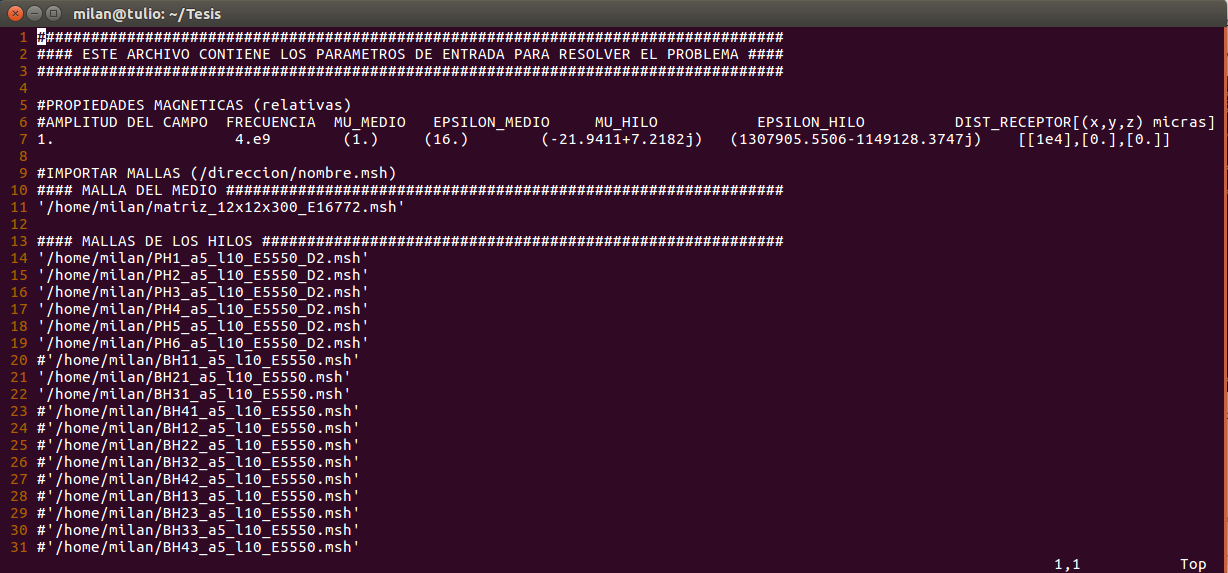
\includegraphics[scale=0.42]{Imagenes/infotxt.png}\\
	\caption{Formato de archivo info.txt con múltiples mallas para facilidad de uso}
	\label{fig:infotxt}
\end{figure} 

\pagebreak
Luego es necesario ejecutar el archivo que creará el programa para resolver el problema, esto se realiza a través un archivo llamado ``conector.py'' que se puede ver en el apéndice B. Finalmente es necesario ejecutar el programa creado llamado ``ejecutor.py'' y leer los los resultados, un ejemplo de este programa se puede ver en el apéndice C para 6 hilos. Es necesario que los archivos ``info.txt'' y ``conector.py'' se encuentren en la misma carpeta al momento de ejecutar cualquier resolución. Los programas recién mencionados se pueden encontrar en \textit{https://github.com/MilanUngerer/BEM\_microwire}.

En este trabajo se utilizó un computador con las siguientes características:
\begin{itemize}
	\item Memoria RAM: 32767 [Mb]
	\item Número de núcleos lógicos: 24
	\item Versión Python: 2.7.6
	\item Versión BEM++: 3.0.3
\end{itemize}

Para una frecuencia de 4[GHz] se puede obtener una longitud de onda ($\lambda$) de 74.95 [mm], un número de onda en el vacío de $8.383\times10^{-5}$, además, las propiedades mostradas en la tabla siguiente,\\

\hspace{-15mm}
\begin{tabular}{ |p{4.78cm}||p{4.6cm}|p{4.8cm}|p{3cm}|  }
	\hline
	\multicolumn{4}{|c|}{\textbf{Tabla de valores}} \\
	\hline
	\textbf{Propiedad} & \textbf{Hilo sin tensión} & \textbf{Hilo con tensión} & \textbf{Matriz}\\
	\hline
	Permitividad ($\epsilon$) [-]  & 400430,875-1139694,314 i   & 1307905,551-1149128,375 i & 16,0\\
	Permeabilidad ($\mu$) [-]&   -21,941+7,218 i  & -21,941+7,218 i & 1,0\\
	Índice de refracción ($n$) [-] & 3697,485+3772,366 i & 3147,337+5505,268 i & 4,0\\
	Índice de transmisión ($\alpha$) [-]   & -21,941+7,218 i & -21,941+7,218 i & 1,0\\
	Número de onda ($k$) [$\mu m^{-1}$] & 1,240+1,265j & 1,055+1,846 i &$3.35\times 10^{-4}$\\
	\hline
\end{tabular}
\\\\

Para las pruebas se utilizó el orden de cuadratura de 6 (por defecto), además, una tolerancia de $10^{-5}$ para la multiplicación matriz-vector a través de GMRES. El máximo de iteraciones está fijado en 50.000 y el valor para el ``restart'' de 5.000. Este último parámetro es muy importante al momento de la convergencia ya que si el valor del ``restart'' es bajo la convergencia no es alcanzada de manera satisfactoria. La recomendación para este caso es fijarlo en un valor alto para no ser ejecutado ya que el valor por defecto es de 20 iteraciones.

\pagebreak
%%%%%%%%%%%%%%%%%%%%%%%%%%%%%%%%%%%%%%%%%%%%%%%%%%%%%%%%%%%
\subsection{Variación del campo variando la distancia entre hilos}
En esta sección se mostrarán los resultados obtenidos al variar la distancia entre los hilos bajo una configuración de pantalla. El número de hilos se mantiene constante durante la experimentación por lo que a menor cantidad se encontrarán concentrados principalmente en el centro de la matriz, a medida que aumenta la distancia entre los hilos estos se encontrarán distribuidos de mejor manera en la matriz. En esta sección se utilizará una configuración de tipo pantalla compuesta por 6 hilos modelados como cilindros de 10[$\mu m$] de diámetro y 10[mm] de largo (según \cite{Wire_theory_1}). Con estos valores se tiene una composición volumétrica de 0.011\%.

Al examinar los resultados con y sin tensión, es necesario comparar además, el módulo de los campos obtenidos, el módulo de un número complejo $z$ se define como:

$$|z| = \sqrt{\left[Re(z)\right]^2+\left[Im(z)\right]^2}$$

Donde $Re(z)$ y $Im(z)$ representan la parte real e imaginaria respectivamente. El valor del módulo es un parámetro de importancia debido a que este se utilizará en la comparación entre los campos con y sin tensión aplicada. El módulo representa la amplitud de la onda $u(\textbf{r})$ en la siguiente ecuación:

$$\textbf{U}(\textbf{r},t) = u(\textbf{r})e^{-i\omega t}$$ 

El cambio entre los campos serán comparados a través de:

$$\frac{C_{ss}-C_{cs}}{C_{ss}} = Cambio\quad de\quad campo$$

\begin{figure}[H]
	\centering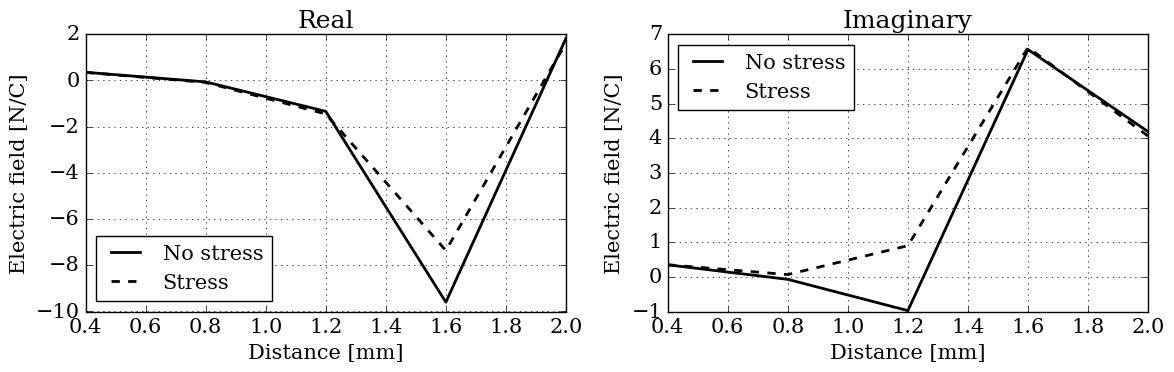
\includegraphics[scale=0.6]{Imagenes/field_screen_comparision.png}\\
\end{figure} 
\begin{figure}[H]
	\centering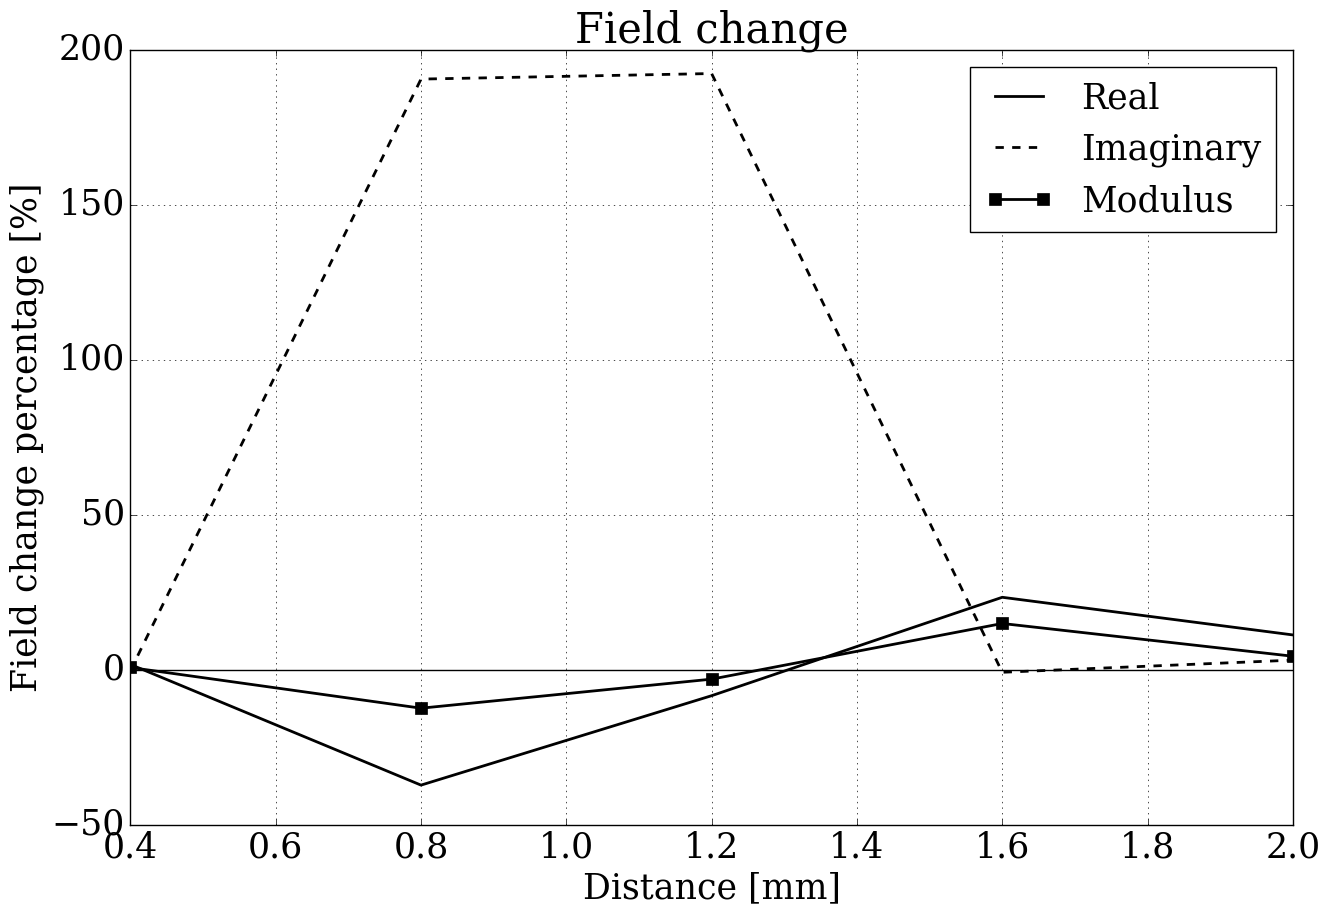
\includegraphics[scale=0.35]{Imagenes/field_change.png}\\
	\caption{Campo y variación del campo obtenido 10[mm] aguas abajo del compósito en función del cambio de distancia entre hilos}
	\label{fig:field_change}
\end{figure}
 
Una vez ejecutado el programa ``ejecutor.py'' se puede encontrar en la carpeta un gráfico con la convergencia del programa como el que se puede ver a continuación,

\begin{figure}[H]
	\centering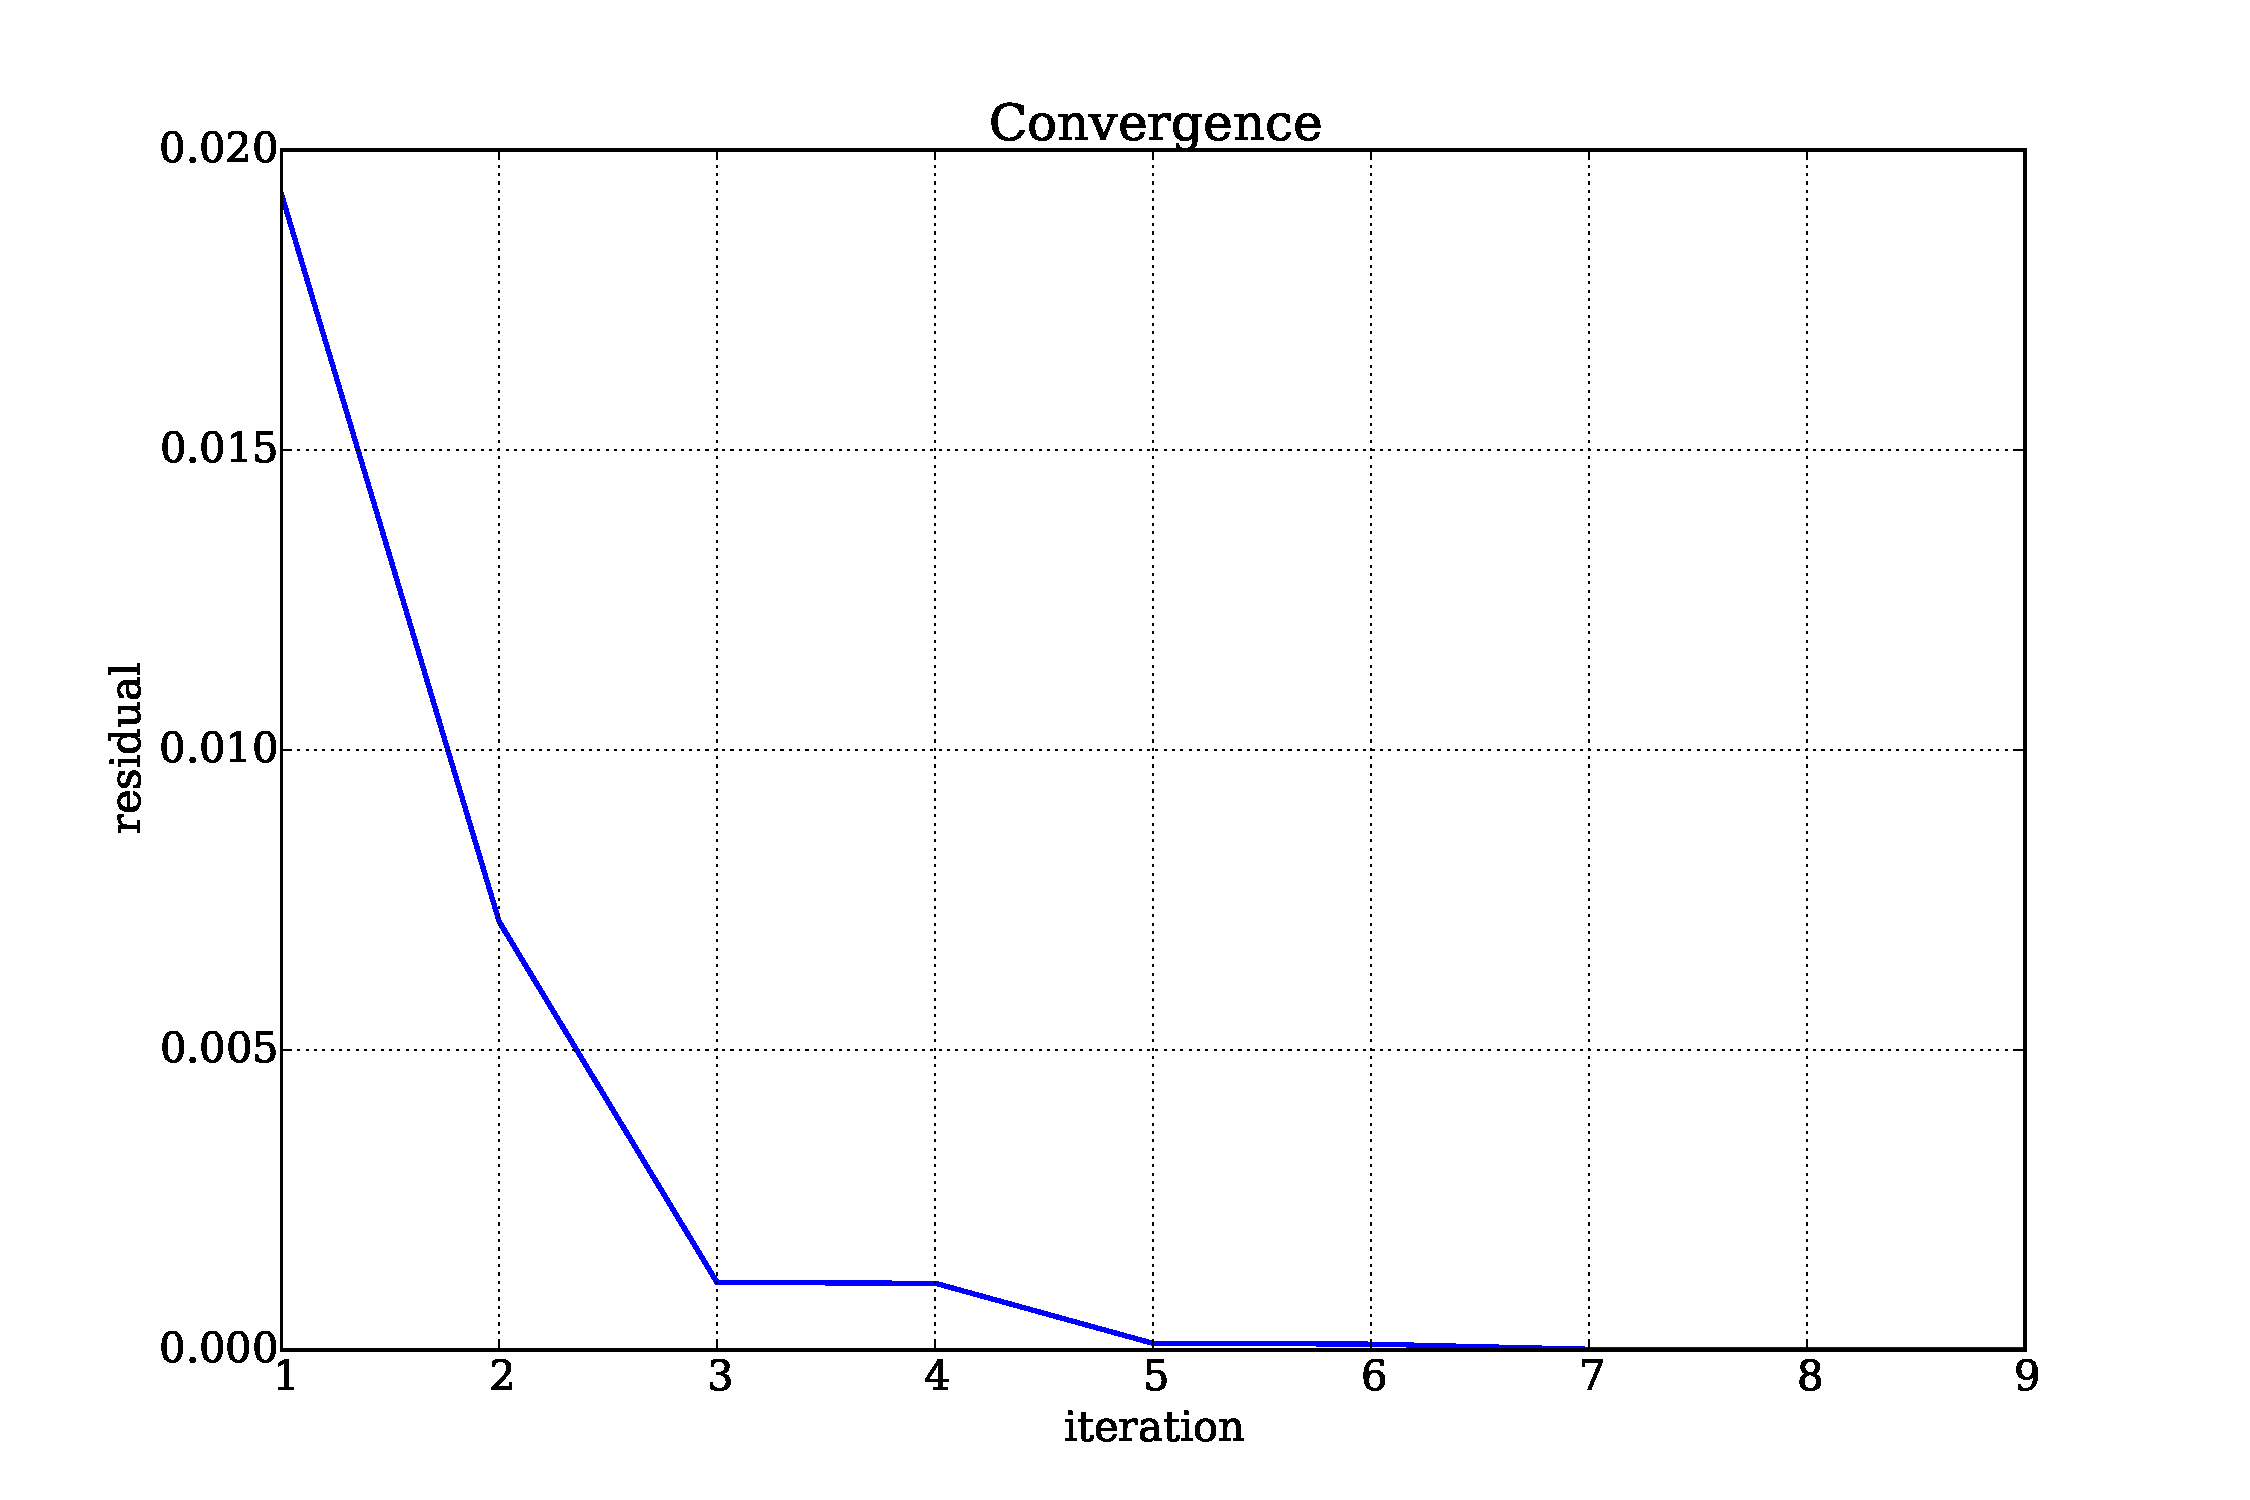
\includegraphics[scale=0.35]{Imagenes/Convergence.pdf}\\
	\caption{Convergencia para llegar a la tolerancia deseada para un GMRES con una matriz sin hilos}
	\label{fig:convergence}
\end{figure} 

%%%%%%%%%%%%%%%%%%%%%%%%%%%%%%%%%%%%%%%%%%%%%%%%%%%%%%%%%%%
\subsection{Variación del campo en función del número de filas}

A continuación se presentan los resultados de la variación del campo eléctrico en función del número de filas. Cada fila contiene 4 hilos detallados en las secciones anteriores.

\begin{figure}[H]
	\centering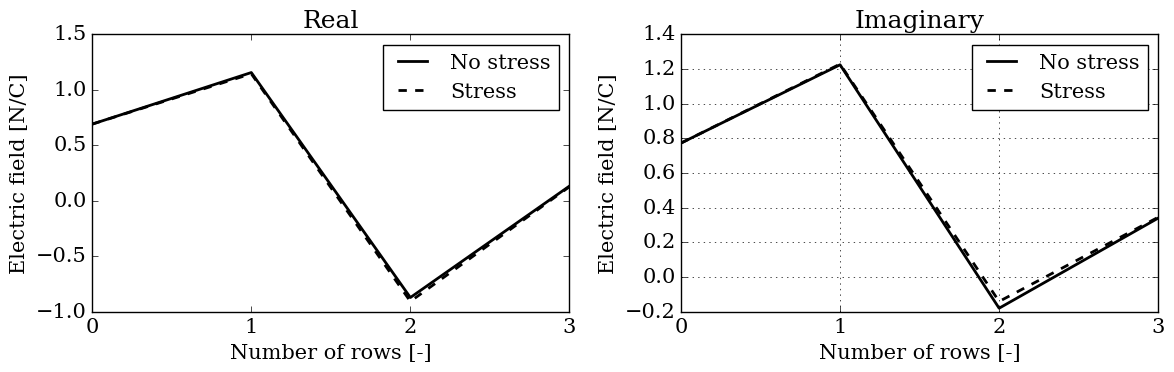
\includegraphics[scale=0.6]{Imagenes/block_comparision.png}\\
\end{figure} 
\begin{figure}[H]
	\centering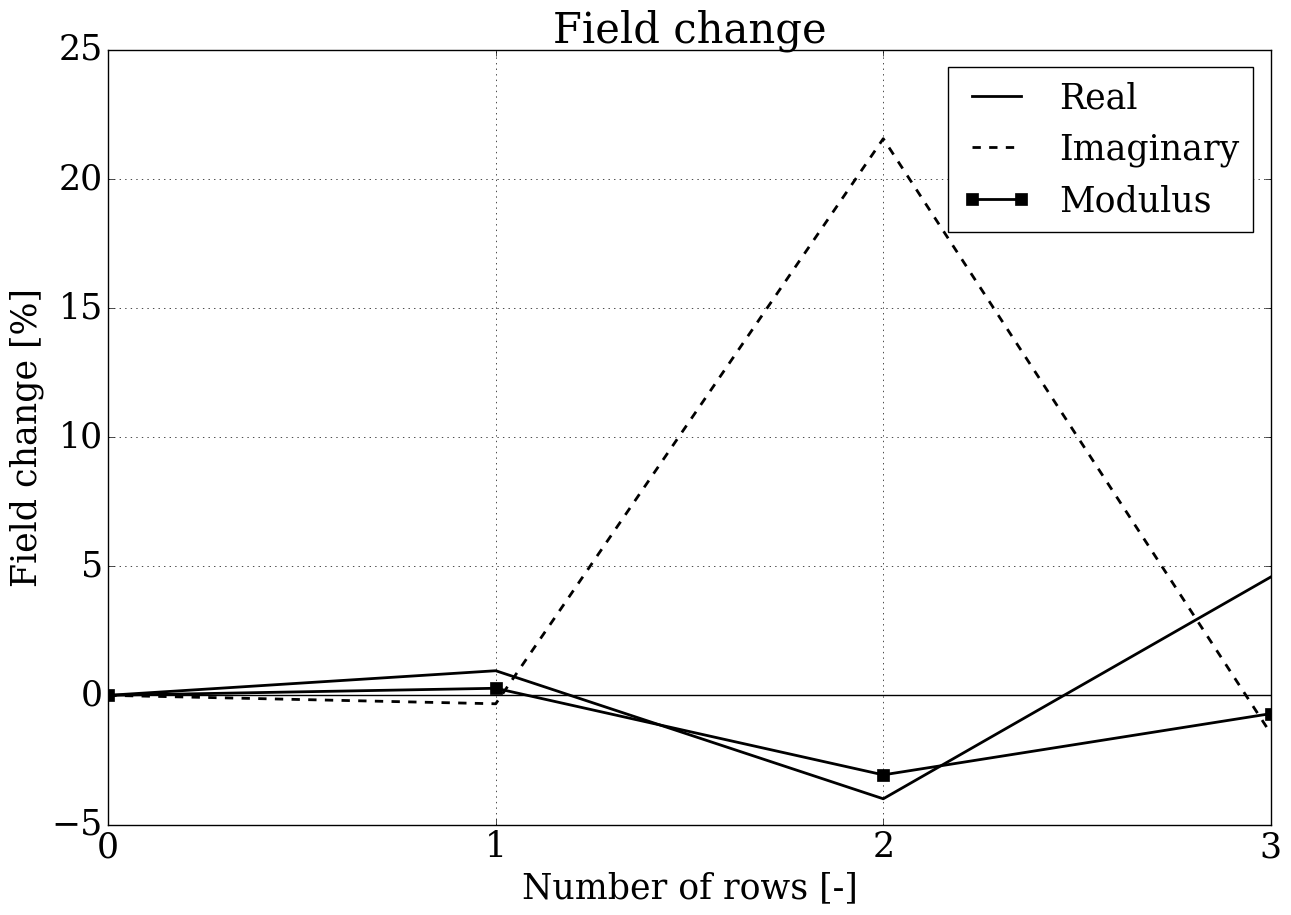
\includegraphics[scale=0.35]{Imagenes/block_change.png}\\
	\caption{Campo y variación del campo obtenido 10[mm] aguas abajo del compósito en función del número de filas del compósito}
	\label{fig:fieldblockchange}
\end{figure}

%%%%%%%%%%%%%%%%%%%%%%%%%%%%%%%%%%%%%%%%%%%%%%%%%%%%%%%%%%%
\subsection{Variación del campo con respecto a la composición volumétrica}
Otro parámetro de interés para maximizar el cambio de señal recibida al modificar las propiedades del compósito es la composición volumétrica, ya que esto podría determinar el porcentaje óptimo para obtener datos más precisos.
Se realizaron múltiples pruebas cambiando el número de hilos al interior de la matriz. El volumen de cada hilo es de $7.85\times 10^{-4}[mm^3]$ y el de la matriz de 43.2 [$mm^3$], por lo que la composición volumétrica es posible obtenerla a través de,

$$\%Vol = nh\times\frac{Vol_h}{Vol_m}$$

Donde $nh$ representa el número de hilos, $Vol_h$ el volumen de cada hilo y $Vol_m$ el volumen de la matriz. 

\begin{figure}[H]
	\centering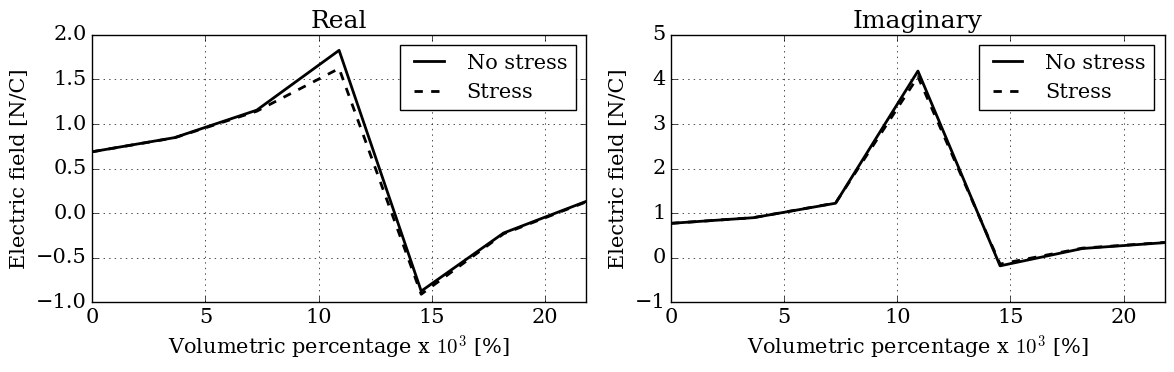
\includegraphics[scale=0.6]{Imagenes/field_vol_comparision.png}\\
\end{figure} 
\begin{figure}[H]
	\centering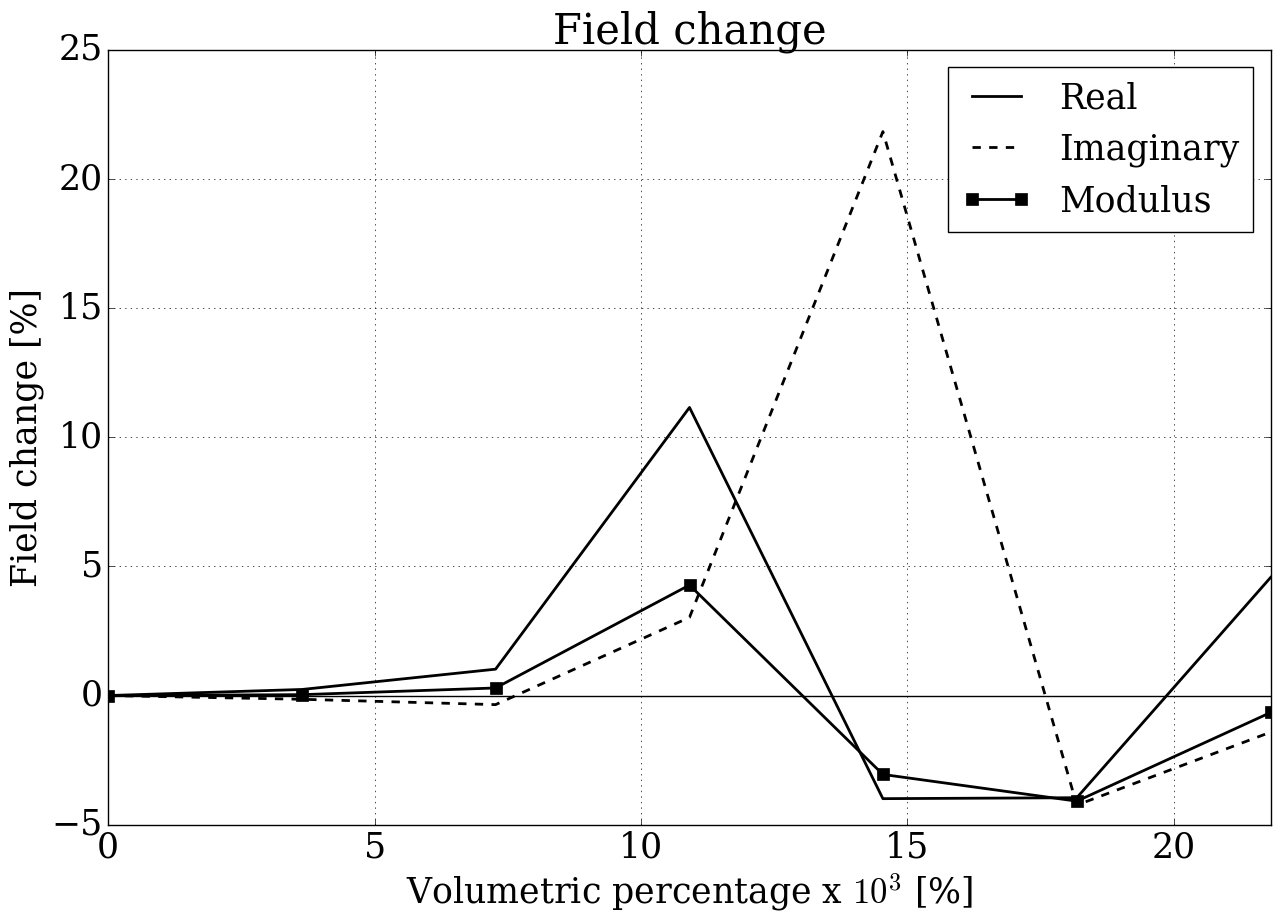
\includegraphics[scale=0.35]{Imagenes/field_vol_change.png}\\
	\caption{Campo y variación del campo obtenido 10[mm] aguas abajo del compósito en función del cambio del porcentaje volumétrico}
	\label{fig:fieldvolchange}
\end{figure}

Otros datos de interés es el tiempo que podría demorar la solución y esto está en directa relación con el número de iteraciones que son necesarias para lograr la tolerancia deseada en el GMRES. Para determinar la capacidad de la máquina a utilizar para ejecutar el programa en función del tamaño de este, se estudia la memoria RAM utilizada con respecto al número de hilos utilizados.\\

\begin{figure}[H]
	\begin{minipage}{0.5\linewidth}
		\centering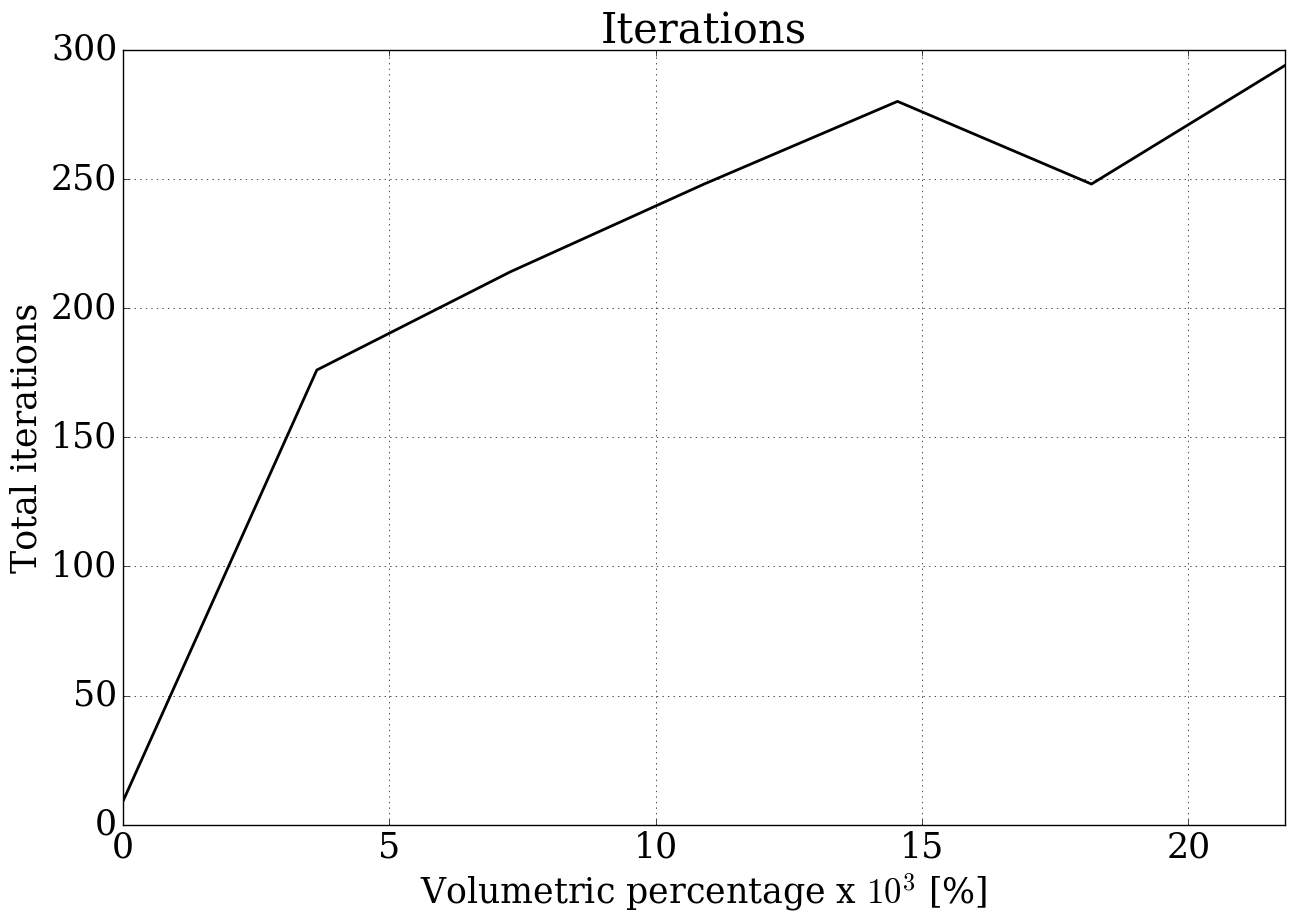
\includegraphics[scale=0.26]{Imagenes/itplot.png}\\
		\centering(a)
	\end{minipage}
	\hspace{5mm}
	\begin{minipage}{0.5\linewidth}
		\centering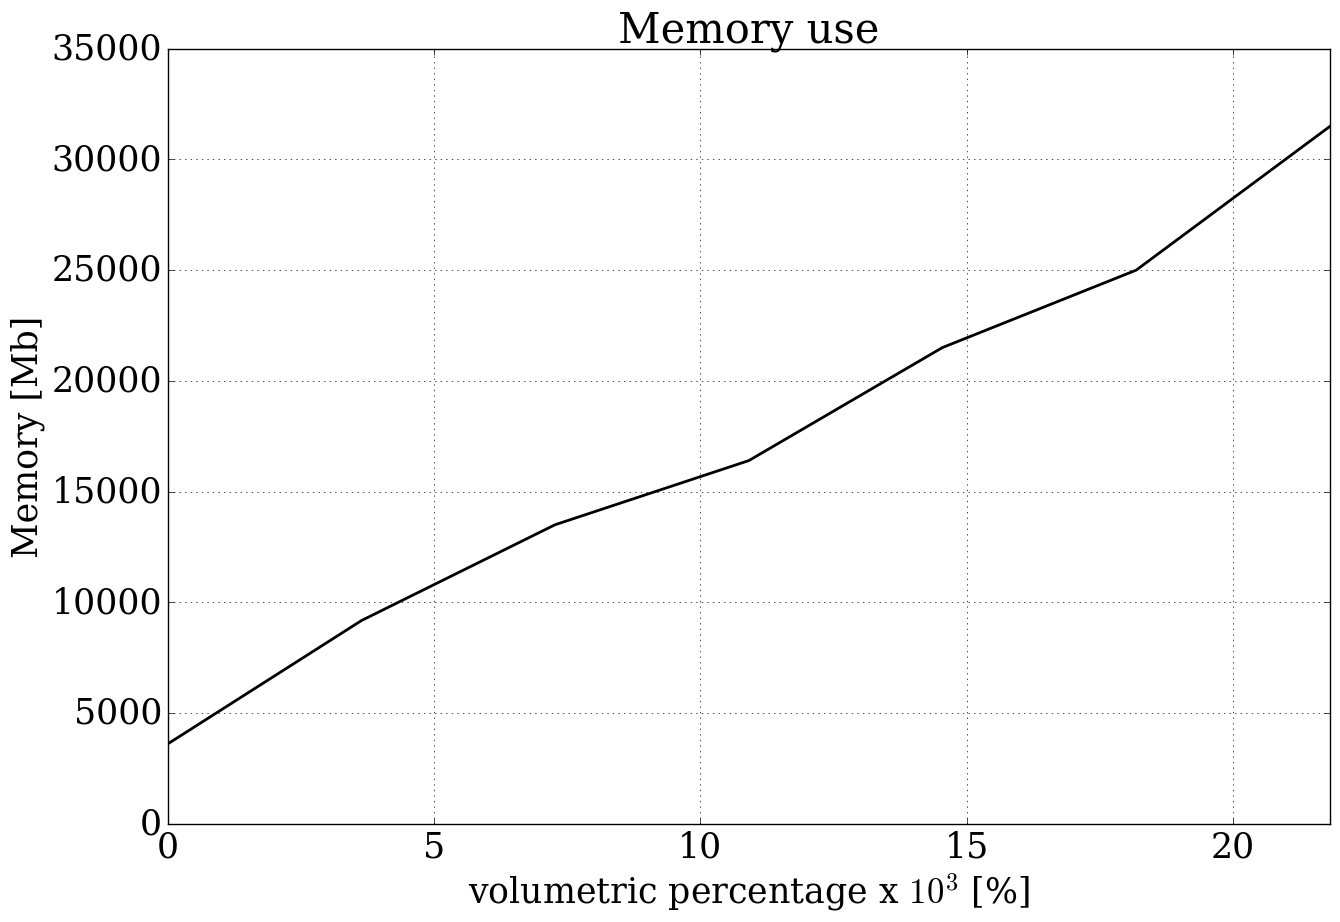
\includegraphics[scale=0.26]{Imagenes/memory.png}\\
		\centering(b)
	\end{minipage}
	\caption{Número de iteraciones y memoria utilizada en función del porcentaje volumétrico}
	\label{fig:itvsnhilos}
\end{figure}

%%%%%%%%%%%%%%%%%%%%%%%%%%%%%%%%%%%%%%%%%%%%%%%%%%%%%%%%%%%
%%%%%%%%%%%%%%%%%%%%%%%%%%%%%%%%%%%%%%%%%%%%%%%%%%%%%%%%%%%
\section{Análisis y conclusiones} \label{sec:Analisis y conclusiones}
En la sección anterior se mostraron los resultados obtenidos para las diferentes configuraciones seleccionadas para realizar las pruebas en la distribución de los hilos. En esta sección se analizarán los resultados.

Para el caso de una configuración de pantalla se puede apreciar que existe un máximo de cambio de señal cuando los hilos se encuentran a 1.6 [mm] con una variación en el módulo de 14.84 \%, Como se puede apreciar en la gráfica \ref{fig:field_change} al encontrarse a 0.8 [mm] existen variaciones de 12.48 \% siendo otro posible valor para posicionar los micro-hilos, el problema con esta última distancia entre hilos es que a pesar que el porcentaje de cambio es alto la diferencia es baja por lo que se dependería de una mejor resolución en el aparato de medición. La recomendación es de posicionar los hilos a una distancia de 1.6 [mm]. 

Para el caso de una configuración de bloque, variando el número de filas, se puede ver que existe un máximo de variación en 2 filas. El problema en este caso es que la diferencia entre los valores y el cambio del campo son bajos alcanzando una variación máxima de tan solo 3.08 \%. Una posible razón de encontrar pequeñas variaciones es el hecho de que el espesor de la matriz es pequeño lo que hace necesario agregar filas muy cercanas unas de otras generando un comportamiento de bloque entre los hilos. Por otro lado, en la bibliografía no se encontró información relativa a añadir más filas en el compósito.

Además, se puede observar que para el porcentaje volumétrico existe un máximo con 0,0109\% (6 hilos) alcanzando un cambio en el módulo de alrededor de 4.28\%. Este resultado coincide con la composición volumétrica utilizada en la cita \cite{Wire_theory_1} y en el estudio del cambio del campo al variar la distancia entre hilos. Otro valor de cambio importante se produce en 18.18\% (10 hilos) alcanzando un cambio en el módulo de -4.09\%, se prefiere la configuración de 6 hilos ya que la diferencia entre campos es mayor. Al aumentar el número de hilos la memoria necesaria para almacenar la resolución del problema aumenta prácticamente de forma lineal. También se puede notar que al aumentar el número de hilos la convergencia del problema se vuelve más demorosa.

Para comparar los resultado se utilizó la frecuencia en que se presentaban mayores cambios y la que seleccionaría para el diseño del sensor. 

Es importante mencionar que los hilos utilizados no son los que se seleccionarían para el diseño del sensor de tensiones mecánicas, esto debido a que estos hilos presentan, como se nombró anteriormente, anisotropía circunferencial lo que los vuelve buenos candidatos para un sensor de campo magnético externo y no de tensiones mecánicas, para este último caso sería necesaria una anisotropía axial o helicoidal. La principal razón de no utilizar en este estudio micro-hilos con la configuración deseada corresponde a la falta de información existente con respecto a las propiedades de los hilos, en particular permitividad, sobretodo cuando se desea calcular el cambio debido a una tensión mecánica. Otra aproximación tomada es el hecho de no cambiar los valores de la permeabilidad magnética al someter los hilos a tensión, de todas maneras en ninguna referencia se ve dependencia entre estos dos parámetros. 

Un parámetro importante a tener en cuenta al momento de crear las geometrías es el hecho de que la matriz y los hilos poseen dimensiones muy diferentes lo que significa una gran diferencia en el tamaño de los elementos de ambas mallas generando problemas de convergencia y ensamblaje. 

En el código propuesto sólo se consideró el cálculo del campo para el exterior del compósito debido a la naturaleza física de la experimentación que se realiza para este tipo de materiales.

Se puede apreciar que el método de elementos de borde presenta grandes ventajas al momento de simular un fenómeno de este tipo, ya que, no es necesario una discretización de todo el espacio sino que sólo del borde de los objetos, disminuyendo el número de incógnitas, lo que hace posible evaluar el campo en cualquier punto una vez que se obtiene la solución al sistema de ecuaciones. Además, el uso de la librería BEM++ facilita enormemente el trabajo realizado siendo necesario sólo manipular los operadores, sin necesidad de hacer el trabajo de creación de operadores directamente, obteniendo un ensamblaje eficiente y efectivo, ahorrando mucho tiempo de trabajo al momento de crear el programa.

Los errores que es posible encontrar, como es propio de cualquier método numérico computacional, son por truncamiento debido a la naturaleza de una aproximación por método numérico y error por redondeo debido a que no es posible almacenar dígitos infinitos en un computador. El error en la solución también es posible atribuirlo a que el modelo utilizado no sea el óptimo para resolver un sistema de este tipo. Para este último punto se podría resolver el sistema a través de la ecuación de Maxwell detallada en la sección 4.1 y comparar los resultados obtenidos.

Se puede concluir que el método de elementos de borde es una excelente herramienta para aproximar ecuaciones de onda mediante la ecuación de Helmholtz.

La utilización de una solución al sistema matriz-vector por medio de GMRES hacen necesario un estudio de este método ya que variar sus parámetros a conveniencia pueden significar fuertes avances en el número de iteraciones. 

El programa desarrollado en este trabajo podría significar una disminución en los costos asociados a los procesos iterativos que significan el diseño de un sensor inalámbrico como el propuesto. Además, podría utilizarse para casos de interés como el comportamiento de un campo producto de la dispersión provocada por una prótesis dental sometida a tensión, aplicaciones en la prueba de neumáticos de camiones, entre otros.

%%%%%%%%%%%%%%%%%%%%%%%%%%%%%%%%%%%%%%%%%%%%%%%%%%%%%%%%%%%
%%%%%%%%%%%%%%%%%%%%%%%%%%%%%%%%%%%%%%%%%%%%%%%%%%%%%%%%%%%
\pagebreak
\pagenumbering{gobble}% Remove page numbers (and reset to 1)

\begin{thebibliography}{9}
	\bibitem{Griffiths} 
	David J. Griffiths. 
	\textit{Introduction to Electrodynamics}. 
	3rd Edition, 1998.
	
	\bibitem{paperBEMpp}
	W. Śmigaj, S. Arridge, T. Betcke, J. Phillips, M. Schweiger, 
	\textit{``Solving Boundary Integral Problems with BEM++'',} 
	ACM Trans. Math. Software 41, pp. $6:1-6:40$ (2015)	
	 
	\bibitem{BEMpp_example}
	S.P. Groth, A.J. Baran, T. Betcke, S. Havemann and W. Śmigaj
	\textit{``The boundary element method for light scattering by ice crystals and its implementation in BEM++'',} 
	Journal of Quantitative Spectroscopy \& Radiative Transfer 167 (2015) 40–52
		
	\bibitem{paginaBEMpp} 
	The BEM++ project,
	\\\texttt{http://www.bempp.org/}
	
	\bibitem{paginaGmsh} 
	The Gmsh project,
	\\\texttt{http://gmsh.info/}		

	\bibitem{BIE_Helmholtz_1}
	R. E. Kleinman and G. F. Roach. 
	\textit{``Boundary integral equations for the three-dimensional Helmholtz equation'',} 
	SIAM Review. Vol. 16, No 2, April 1974.
	
	\bibitem{BIE_Helmholtz_2}
	S. Amini and S. M. Kirkup. 
	\textit{``Solution of Helmholtz equation in the exterior domain by elementary boundary integral methods'',} 
	Journal of computational physics 118, 208-221 (1995).	 	
	
	\bibitem{Multiple scattering} 
	P. A. Martin. 
	\textit{Multiple scattering, Interaction of Time-Harmonic Waves with N obstacles}. 
	1st Edition, 2006.
	
	\bibitem{Multitrace_acoustic}
	Xavier Claeys and Ralf Hiptmair. 
	\textit{``Multi-Trace Boundary Integral Formulation for Acoustic Scattering by Composite Structures'',} 
	Communications on Pure and Applied Mathematics, Vol. LXVI, 1163-1201 (2013).
	
	\bibitem{Multitrace_electromagnetic}
	Xavier Claeys and Ralf Hiptmair. 
	\textit{``Electromagnetic Scattering at composite objects: A Novel Multi-Trace Boundary Integral Formulation'',} 
	ESAIM: M2AN 46 (2012) 1421-1445
	
	\bibitem{Wire_theory_1}
	D. P. Markhnovskiy and L. V. Panina.
	\textit{``Field dependent permittivity of composite materials containing ferromagnetic wires'',} 
	Journal of applied Physics 93, 4120 (2003).
	
	\bibitem{Wire_theory_2}
	D. P. Markhnovskiy and L. V. Panina.
	\textit{``Experimental demonstration of tunable scattering spectra at microwave frequencies in composite media containing CoFeCrSiB glass-coated amorphous ferromagnetic wires and comparison with theory'',} 
	Physical Review B 74, 064205 (2006).
	
	\bibitem{Wire_intro}
	Faxiang Qin and Hua-Xin Peng.
	\textit{``Ferromagnetic microwires enabled multifunctional composite materials'',} 
	Progress in Materials Science 58 (2013) 183-259.		

	\bibitem{Wire_backgound}
	Faxiang Qin, C. Brosseau, and H. X. Peng.
	\textit{``In situ microwave characterization of microwire composites under mechanical stress'',} 
	Appl. Phys. Lett. 99, 252902 (2011).
	
	\bibitem{Wire_permeability}
	L. Liu, K.N. Rozanov and M. Abshinova
	\textit{``Tunable properties of microwire composites at microwave frequency'',} 
	Appl. Phys. A (2013) 110:275-279.		

\end{thebibliography}

\pagebreak
%Introducción a la base matemática que será utilizada
\part*{Apéndice A: Análisis vectorial}
%\section*{Análisis vectorial}
\setcounter{figure}{0}

Para entender la matemática que describe una onda electromagnética y el análisis numérico utilizado en este trabajo, es necesario antes, introducir algunos conceptos de análisis vectorial que serán útiles, es por esto que primero definiremos el concepto de vector.\\

\noindent Un vector es una magnitud física definida en un sistema de referencia, que se caracteriza por tener módulo, dirección y sentido. Se puede representar mediante una combinación de los componentes del sistema de referencia.

$$\vec{A}=A_x\hat{x}+A_y\hat{y}+A_z\hat{z}$$

\noindent Donde $A$ es un vector arbitrario representado según  $\hat{x}$, $\hat{y}$ y $\hat{z}$ vectores unitarios paralelos al eje $x$, $y$ y $z$ respectivamente considerando coordenadas cartesianas. También puede ser representado mediante una tupla de $n$ números reales, siendo $n$ la dimensión del vector, es decir, su número de componentes.

$$\vec{A}=(A_x,A_y,A_z)$$

\noindent En el plano cartesiano quedaría representado por la fig. \ref{Fig:Vectores} (b). 

\begin{figure}[h!]
	\centering\includegraphics[scale=0.5]{Imagenes/Vectores.png}
	\caption{Representación gráfica de un vector en el plano cartesiano}
	\label{Fig:Vectores}
\end{figure}

%%%%%%%%%%%%%%%%%%%%%%%%%%%%%%%%%%%%%%%%%%%%%%%%%%%%%%%%%%%
\section*{Álgebra vectorial}
Al igual que una magnitud escalar es posible realizar operaciones algebraicas con vectores, pero hay que tener en consideración algunas reglas básicas. 

\begin{enumerate}
	\item Suma
	$$\vec{A}+\vec{B}=(A_x+B_x)\hat{x}+(A_y+B_y)\hat{y}+(A_z+B_z)\hat{z}$$
	
	\item Resta
	$$\vec{A}-\vec{B}=(A_x-B_x)\hat{x}+(A_y-B_y)\hat{y}+(A_z-B_z)\hat{z}$$
	
	\item Multiplicación por un escalar
	$$a\vec{A}=aA_x\hat{x}+aA_y\hat{y}+aA_z\hat{z}$$
	
	\item Producto punto
	$$\vec{A}\cdot\vec{B}=A_xB_x+A_yB_y+A_zB_z$$
	
	\item Producto cruz
	$$\vec{A}\times\vec{B}=\left | \begin{array}{ccc}
	\hat{x} & \hat{y} & \hat{z}\\
	A_x & A_y & A_z\\
	B_x & B_y & B_z  \end{array} \right |$$
	
\end{enumerate}

%%%%%%%%%%%%%%%%%%%%%%%%%%%%%%%%%%%%%%%%%%%%%%%%%%%%%%%%%%%
\section*{Vector Posición}
El vector posición corresponde al vector que va desde el origen hasta un punto arbitrario. En coordenadas cartesianas se puede definir de la siguiente manera.

$$\vec{r}\equiv x\hat{x}+y\hat{y}+z\hat{z}$$

\noindent La magnitud de este vector es la distancia entre el punto y el origen del eje de coordenadas, se puede calcular mediante la siguiente expresión.

$$r=|\vec{r}|=\sqrt{x^2+y^2+z^2}$$

\noindent El vector unitario en dirección a $\vec{r}$ puede calcularse mediante:

$$\hat{r}=\frac{\vec{r}}{r}=\frac{x\hat{x}+y\hat{y}+z\hat{z}}{\sqrt{x^2+y^2+z^2}}$$

\noindent Para la aplicación del método de elementos de borde es necesario utilizar vectores que vayan desde un punto en el borde de la geometría a estudiar hasta otro punto arbitrario, es por esto que se define el vector separación como una resta entre ambos puntos en cuestión.

\begin{figure}[H]\label{fig:ell}
	\centering\begin{tikzpicture}[scale=1]
	\draw[->] (-0.5,0) -- (3.5,0) node[below] {$x$};
	\draw[->] (0,-0.5) -- (0,3.5) node[left] {$y$};
	\draw[thick, ->] (0,0) -- (2,3);
	\draw[thick, ->] (0,0) -- (3,2);
	\draw[thick, ->] (2,3) -- (3,2);
	\draw (0.7,2.2) -- (0.7,2.2) node[anchor=north] {$\vec{r'}$};
	\draw (2,1) -- (2,1) node[anchor=north] {$\vec{r}$};
	\draw (2.8,3) -- (2.8,3) node[anchor=north] {$\vec{\ell}$};
	\end{tikzpicture}
	\caption{Representación vector $\vec{\ell}$}
\end{figure}

%%%%%%%%Paso de página%%%%%%%%%%
\pagebreak
%%%%%%%%%%%%%%%%%%%%%%%%%%%%%%%%

Se puede definir este vector separación en función del vector posición.

$$\vec{\ell}=\vec{r}-\vec{r'}$$ 

\noindent Con magnitud,

$$\ell=|\vec{r}-\vec{r'}|$$

\noindent y vector unitario, 

$$\hat{\ell}=\frac{\vec{\ell}}{\ell}=\frac{\vec{r}-\vec{r'}}{|\vec{r}-\vec{r'}|}$$

%%%%%%%%%%%%%%%%%%%%%%%%%%%%%%%%%%%%%%%%%%%%%%%%%%%%%%%%%%%
\section*{Cálculo diferencial}

Se define un operador diferencial $\nabla$, que servirá para introducir derivadas en forma vectorial, según la siguiente expresión.

$$\nabla\equiv\frac{\partial}{\partial x}\hat{x}+\frac{\partial}{\partial y}\hat{y}+\frac{\partial}{\partial z}\hat{z}$$ 

\noindent Aunque claramente no es un vector de la forma tradicional, se pueden utilizar las reglas básicas del álgebra vectorial con este operador. De esta manera $\nabla$ puede actuar de tres formas.

\begin{enumerate}
	\item Sobre una función escalar T: $\nabla T$ (Gradiente)
	\item Sobre una función vectorial $v$, mediante un producto punto: $\nabla\cdot v$ (Divergencia)
	\item Sobre una función vectorial $v$, mediante un producto cruz: $\nabla\times v$ (Rotor)
\end{enumerate}

\noindent Este operador puede aplicar sobre si mismo, como es el caso del operador de LaPlace, que corresponde a la divergencia de la gradiente de una función $T$.

$$\nabla^2 T=\nabla\cdot (\nabla T)=\frac{\partial^2 T}{\partial x^2}+\frac{\partial^2 T}{\partial y^2}+\frac{\partial^2 T}{\partial z^2}$$

\noindent Otra aplicación relevante del operador $\nabla$ sobre si mismo es el caso del rotor sobre la gradiente, resultando siempre nulo.

$$\nabla\times(\nabla T)=0$$

%%%%%%%%Paso de página%%%%%%%%%%
\pagebreak
%%%%%%%%%%%%%%%%%%%%%%%%%%%%%%%%
%%%%%%%%%%%%%%%%%%%%%%%%%%%%%%%%%%%%%%%%%%%%%%%%%%%%%%%%%%%%%%
\section*{Cálculo integral}
Si se le aplica el concepto de integral a funciones que tienen una forma diferencial, se pueden obtener algunos teoremas que se usarán más adelante en el planteamiento del método de elementos de borde.

\begin{enumerate}
	\item Teorema fundamental del cálculo
	$$\int_{a}^{b}\frac{df}{dx}dx=f(b)-f(a)$$
	\item Teorema fundamental de la gradiente
	$$\int_{a}^{b}\nabla Tdl=T(b)-T(a)$$
	\item Teorema fundamental de la divergencia (Teorema de Gauss)
	$$\int_{\Omega}(\nabla\cdot v)d\varOmega=\oint_{\Gamma}v\cdot d\varGamma$$
	\item Teorema fundamental del rotor (Teorema de Stokes)
	$$\int_{\Gamma}(\nabla\times v)\cdot d\varGamma=\oint_{P}v\cdot dl$$ 
\end{enumerate}

\noindent Aplicando estos teoremas en conjunto con algunas reglas del producto del cálculo vectorial, se pueden obtener formulaciones generales que más adelante será necesario utilizar.

$$\nabla\cdot (fA)=f(\nabla\cdot A)+A\cdot (\nabla f)$$

\noindent Integrando sobre el volumen, se obtiene,

$$\int_{\Omega}\nabla\cdot (fA)d\varOmega=\int_{\Omega}f(\nabla\cdot A)d\varOmega+\int_{\Omega}A\cdot (\nabla f)d\varOmega=\oint_\Gamma fA\cdot d\varGamma$$

\noindent Reordenando se llega a,
\begin{equation}
\int_{\Omega}f(\nabla\cdot A)d\varOmega=-\int_{\Omega}A\cdot (\nabla f)d\varOmega+\oint_\Gamma fA\cdot d\varGamma
\label{eq: gaussdiv}	
\end{equation}

%%%%%%%%Paso de página%%%%%%%%%%
\pagebreak
%%%%%%%%%%%%%%%%%%%%%%%%%%%%%%%%
%%%%%%%%%%%%%%%%%%%%%%%%%%%%%%%%%%%%%%%%%%%%%%%%%%%%%%%%%%%%%%
\subsection*{Función delta Dirac} \label{dirac}
Se abarcará este punto de manera más extensa ya que se considera que es una parte fundamental para la implementación del método de elementos de contorno. Se considera una función vectorial de la forma,
$$\vec{v}=\frac{1}{r^2}\hat{r}$$

\noindent ahora, calculando la divergencia de $\vec{v}$ se obtiene,

$$\nabla\cdot \vec{v}=0$$

\noindent Por otro lado si se resuelve,

$$\oint_\Gamma \vec{v}\cdot d\varGamma=4\pi$$

\noindent Pero la integral $\int_{\Omega}\nabla\cdot \vec{v} d\varOmega=0$, esto significaría que el teorema de Gauss no se estaría cumpliendo, pero se sabe que esto no es posible. La cuestión es que cuando $r=0$ la función $\vec{v}$ crece hacía el infinito, por lo que $\nabla\cdot \vec{v}=0$ en todos lados excepto en el origen.

\begin{figure}[H]\label{fig:dirac}
	\centering\begin{tikzpicture}[scale=1]
	\draw[<->] (-3.0,0) -- (3.0,0) node[below] {$x$};
	\draw[->] (0,0) -- (0,3.5);
	\draw (-1.5,0) parabola (-0.4,0.1);
	\draw (1.5,0) parabola (0.4,0.1);
	\draw (-0.4,0.1) parabola (-0.15,0.5);
	\draw (0.4,0.1) parabola (0.15,0.5);
	\draw (-0.15,0.5) -- (-0.15,2.5);
	\draw (0.15,0.5) -- (0.15,2.5);
	\draw (0,3) parabola (-0.15,2.5);
	\draw (0,3) parabola (0.15,2.5);
	\draw (0,3)  node[right] {$\delta(x)$};		
	\end{tikzpicture}
	\caption{Función $\delta(x)$ en una dimensión}
\end{figure}

\noindent En una dimensión la función delta Dirac queda,

$$\delta(x)=\begin{cases}
0,&\quad \text{Si }x\neq0\\
\infty,&\quad \text{Si }x=0
\end{cases}$$

\noindent donde,

$$\int_{-\infty}^{\infty}\delta(x)dx=1$$

\noindent Si se multiplica la función $\delta(x)$ por otra función continua arbitraria $f(x)$, el producto es cero en todos lados excepto en el origen.

$$f(x)\delta(x)=f(0)\delta(x)$$ 

\noindent Por lo que al integrar resulta,

$$\int_{-\infty}^{\infty}f(x)\delta(x)dx=f(0)$$

Ahora, si se desea trasladar la función delta Dirac a otro punto $x=a$, resulta

$$\delta(x-a)=\begin{cases}
0,&\quad \text{Si }x\neq a\\
\infty,&\quad \text{Si }x=a
\end{cases}$$
Donde,
$$\int_{-\infty}^{\infty}f(x)\delta(x-a)dx=f(a)$$

\noindent En 3 dimensiones se puede expresar la función delta como,

$$\delta^3(\vec{r})=\delta(x)\delta(y)\delta(z)$$

\noindent Al igual que antes la función $\delta(\vec{r})$ es cero en todas partes excepto en $(0,0,0)$.

$$\int_{\Omega}\delta^3(\vec{r})d\varOmega=\int_{-\infty}^{\infty}\int_{-\infty}^{\infty}\int_{-\infty}^{\infty}\delta(x)\delta(y)\delta(z)dxdydz=1$$

\noindent Generalizando,

$$\int_{\Omega}f(\vec{r})\delta^3(\vec{r}-\vec{a})d\varOmega=f(\vec{a})$$

\noindent Como se pudo observar $\nabla\cdot (\hat{r}/r^2)$ es cero en cualquier lugar excepto en el origen, y la integral de cualquier volumen que contenga el origen es constante ($4\pi$), ahora se puede definir, 

$$\nabla\cdot (\frac{\hat{r}}{r^2})=4\pi\delta^3(\vec{r})$$

\noindent o más general,

$$\nabla\cdot (\frac{\hat{\ell}}{\ell^2})=4\pi\delta^3(\vec{\ell})$$

\noindent Donde, como siempre $\vec{\ell}=\vec{r}-\vec{r'}$ y la diferenciación es con respecto a $\vec{r}$, dejando $\vec{r'}$ como constante.

%%%%%%%%%%%%%%%%%%%%%%%%%%%%%%%%%%%%%%%%%%%%%%%%%%%%%%%%%%%
\pagebreak
%Introducción a la base matemática que será utilizada
\part*{Apéndice B: Código automatizado}
%\section*{Análisis vectorial}
\setcounter{figure}{0}
\begin{lstlisting}
1 ################################################################
2 ###### ACA SE LEE EL PROGRAMA QUE CONTIENE LA INFORMACION ######
3 ################################################################
4 import numpy as np
5 
6 info = []
7 for line in open("info.txt"):
8     li=line.strip()
9     if not li.startswith("#"): #Comentarios empiezan con '#'
10         info.append(line.split())
11 
12 info = filter(None, info)
13 #print info
14 N_hilos = len(info) - 2
15 print '\nEl composito contiene', N_hilos, 'microhilos\n'
16 
17 
18 ################################################################
19 ###### ACA SE ESCRIBE EL PROGRAMA PARA EJECUTAR EL CALCULO #####
20 ################################################################
21 exe = open('ejecutor.py','w')
22 
23 ###### IMPORTANDO LIBRERIAS ####################################
24 exe.write('#Preambulo\n')
25 exe.write('import numpy as np\n')
26 exe.write('import bempp.api\n')
27 
28 ###### PARAMETROS DE ENTRADA ###################################
29 #exe.write('bempp.api.global_parameters.quadrature.double_singular = 7\n') #Orden de cuadratura
30 exe.write('omega = 2.*np.pi*' + info[0][1] + '\n') #frecuencia angular
31 exe.write('e0 = 8.854*1e-12*1e-18\n') #permitividad del vacio
32 exe.write('mu0 = 4.*np.pi*1e-7*1e6\n') #permeabilidad del vacio
33 exe.write('mue = ' + info[0][2] + '*mu0\n') #permeabilidad de la matriz
34 exe.write('ee = ' + info[0][3] + '*e0\n') #permitividad de la matriz
35 exe.write('mui = ' + info[0][4] + '*mu0\n') #permeabilidad del conductor
36 exe.write('ei = ' + info[0][5] + '*e0\n') #permitividad del conductor
37 exe.write('k = omega*np.sqrt(e0*mu0)\n') #numero de onda exterior
38 exe.write('lam = 2*np.pi/k\n') #longitud de onda al exterior
39 exe.write('nm = np.sqrt((ee*mue)/(e0*mu0))\n') #indice de refraccion matriz
40 exe.write('nc = np.sqrt((ei*mui)/(e0*mu0))\n') #indice de refraccion conductor
41 exe.write('alfa_m = mue/mu0\n') #indice de transmision matriz
42 exe.write('alfa_c = mui/mue\n') #indice de transmision conductor
43 exe.write('antena = np.array('+info[0][6]+')\n') #Punto antena receptor
44 
45 ###### ESCRIBIR VALORES DE INTERES #############################
46 exe.write('print "Numero de onda exterior:", k\n')
47 exe.write('print "Indice de refraccion matriz:", nm\n')
48 exe.write('print "Indice de refraccion conductor:", nc\n')
49 exe.write('print "Numero de onda interior matriz:", nm*k\n')
50 exe.write('print "Numero de onda interior conductor:", nm*nc*k\n')
51 exe.write('print "Indice de transmision matriz:", alfa_m\n')
52 exe.write('print "Indice de transmision conductor:", alfa_c\n')
53 exe.write('print "Longitud de onda:", lam, "micras"\n')
54 
55 ###### IMPORTANDO MALLAS #######################################
56 exe.write('\n#Importando mallas\n')
57 
58 exe.write('matriz = bempp.api.import_grid('+info[1][0]+')\n') #Malla de la matriz
59 for i in range(N_hilos): #Mallas de hilos
60     exe.write('grid_'+str(i)+' = bempp.api.import_grid('+info[i+2][0]+')\n')
61 
62 ###### FUNCIONES DIRICHLET Y NEUMANN ###########################
63 exe.write('\n#Funciones de dirichlet y neumann\n')
64 
65 exe.write('def dirichlet_fun(x, n, domain_index, result):\n')
66 exe.write('\tresult[0] = '+info[0][0]+'*np.exp(1j*k*x[0])\n')
67 
68 exe.write('def neumann_fun(x, n, domain_index, result):\n')
69 exe.write('\tresult[0] = '+info[0][0]+'*1j*k*n[0]*np.exp(1j*k*x[0])\n')
70 
71 ###### OPERADORES EN EL BORDE ##################################
72 exe.write('\n#Operadores multitrazo\n')
73 exe.write('Ai_m = bempp.api.operators.boundary.helmholtz.multitrace_operator(matriz, nm*k)\n') #Operador multitrazo interior matriz
74 exe.write('Ae_m = bempp.api.operators.boundary.helmholtz.multitrace_operator(matriz, k)\n') #Operador multitrazo exterior matriz
75 for i in range(N_hilos): #Operadores multitrazo hilos
76     exe.write('Ai_'+str(i)+' = bempp.api.operators.boundary.helmholtz.multitrace_operator(grid_' + str(i) + ',nm*nc*k)\n') #Interior hilos
77     exe.write('Ae_'+str(i)+' = bempp.api.operators.boundary.helmholtz.multitrace_operator(grid_' + str(i) + ',nm*k)\n') #Exterior hilos
78 
79 exe.write('\n#Transmision en Multitrazo\n')
80 
81 exe.write('Ae_m[0,1] = Ae_m[0,1]*(1./alfa_m)\n') #Transmision en matriz exterior
82 exe.write('Ae_m[1,1] = Ae_m[1,1]*(1./alfa_m)\n') #Transmision en matriz exterior
83 for i in range(N_hilos): #Transmision en Multitrazo en hilos
84     exe.write('Ai_'+str(i)+'[0,1] = Ai_'+str(i)+'[0,1]*alfa_c\n') #Transmision interior hilos
85     exe.write('Ai_'+str(i)+'[1,1] = Ai_'+str(i)+'[1,1]*alfa_c\n') #Transmision interior hilos
86 
87 exe.write('\n#Acople interior y exterior\n')
88 exe.write('op_m = (Ai_m + Ae_m)\n') #Interior + exterior matriz
89 for i in range(N_hilos): #Interior + exterior hilos
90     exe.write('op_'+str(i)+' = (Ai_'+str(i)+' + Ae_'+str(i)+')\n')
91 
92 exe.write('\n#Espacios\n')
93 exe.write('dirichlet_space_m = Ai_m[0,0].domain\n') #Espacio de dirichlet en matriz
94 exe.write('neumann_space_m = Ai_m[0,1].domain\n') #Espacio de neumann en matriz
95 for i in range(N_hilos): #Espacios en hilos
96     exe.write('dirichlet_space_'+str(i)+' = Ai_'+str(i)+'[0,0].domain\n') #Espacio de dirichlet en hilos
97     exe.write('neumann_space_'+str(i)+' = Ai_'+str(i)+'[0,1].domain\n') #Espacio de neumann en hilos
98 
99 #operadores identidad
100 exe.write('\n#Operadores identidad\n')
101 exe.write('ident_m = bempp.api.operators.boundary.sparse.identity(neumann_space_m, neumann_space_m, neumann_space_m)\n') #Operador identidad matriz
102 for i in range(N_hilos): #Operadores identidad en hilos
103     exe.write('ident_'+str(i)+' = bempp.api.operators.boundary.sparse.identity(neumann_space_' + str(i) + ', neumann_space_' + str(i) + ', neumann_space_' + str(i) + ')\n') #Identidad
104 
105 #operadores diagonales
106 exe.write('\n#Operadores diagonales\n')
107 exe.write('op_m[1,1] = op_m[1,1] + 0.5 * ident_m * ((alfa_m -1)/alfa_m)\n')
108 for i in range(N_hilos):
109     exe.write('op_'+str(i)+'[1,1] = op_' + str(i) + '[1,1] + 0.5 * ident_' + str(i) + '* (alfa_c - 1)\n')
110 
111 #Operadores entre mallas
112 exe.write('\n#Operadores entre mallas\n')
113 for i in range(N_hilos): #Operadores entre mallas 
114     exe.write('SLP_m_'+str(i)+' = bempp.api.operators.boundary.helmholtz.single_layer(neumann_space_m, dirichlet_space_'+str(i)+', dirichlet_space_'+str(i)+', nm*k)\n') #Operadores matriz-hilos single layer
115     exe.write('SLP_'+str(i)+'_m = bempp.api.operators.boundary.helmholtz.single_layer(neumann_space_'+str(i)+', dirichlet_space_m, dirichlet_space_m, nm*k)\n') #Operadores matriz-hilos single layer
116 
117     exe.write('DLP_m_'+str(i)+' = bempp.api.operators.boundary.helmholtz.double_layer(dirichlet_space_m, dirichlet_space_'+str(i)+', dirichlet_space_'+str(i)+', nm*k)\n') #Operadores matriz-hilos double layer
118     exe.write('DLP_'+str(i)+'_m = bempp.api.operators.boundary.helmholtz.double_layer(dirichlet_space_'+str(i)+', dirichlet_space_m, dirichlet_space_m, nm*k)\n') #Operadores matriz-hilos double layer
119 
120     exe.write('ADLP_m_'+str(i)+' = bempp.api.operators.boundary.helmholtz.adjoint_double_layer(neumann_space_m, neumann_space_'+str(i)+', neumann_space_'+str(i)+', nm*k)\n') #Operadores matriz-hilos adjoint double layer
121     exe.write('ADLP_'+str(i)+'_m = bempp.api.operators.boundary.helmholtz.adjoint_double_layer(neumann_space_'+str(i)+', neumann_space_m, neumann_space_m, nm*k)\n') #Operadores matriz-hilos adjoint double lay    er
122 
123     exe.write('HYP_m_'+str(i)+' = bempp.api.operators.boundary.helmholtz.hypersingular(dirichlet_space_m, neumann_space_'+str(i)+', neumann_space_'+str(i)+', nm*k)\n') #Operadores matriz-hilos hypersingular
124     exe.write('HYP_'+str(i)+'_m = bempp.api.operators.boundary.helmholtz.hypersingular(dirichlet_space_'+str(i)+', neumann_space_m, neumann_space_m, nm*k)\n') #Operadores matriz-hilos hypersingular
125 
126     for j in range(N_hilos): #Interaccion entre hilos
127         if i!=j:
128             exe.write('SLP_'+str(i)+'_'+str(j)+' = bempp.api.operators.boundary.helmholtz.single_layer(neumann_space_'+str(i)+', dirichlet_space_'+str(j)+', dirichlet_space_'+str(j)+', nm*k)\n') #Single-layer     interaccion entre hilos
129             exe.write('DLP_'+str(i)+'_'+str(j)+' = bempp.api.operators.boundary.helmholtz.double_layer(dirichlet_space_'+str(i)+', dirichlet_space_'+str(j)+', dirichlet_space_'+str(j)+', nm*k)\n') #Double-lay    er interaccion entre hilos
130             exe.write('ADLP_'+str(i)+'_'+str(j)+' = bempp.api.operators.boundary.helmholtz.adjoint_double_layer(neumann_space_'+str(i)+', neumann_space_'+str(j)+', neumann_space_'+str(j)+', nm*k)\n') #Adjoint     interaccion entre hilos
131             exe.write('HYP_'+str(i)+'_'+str(j)+' = bempp.api.operators.boundary.helmholtz.hypersingular(dirichlet_space_'+str(i)+', neumann_space_'+str(j)+', neumann_space_'+str(j)+', nm*k)\n') #Hypersingular     interaccion entre hilos
132 
133 
134 ###### ENSAMBLANDO MATRIZ DE OPERADORES ########################
135 exe.write('\n#Matriz de operadores\n')
136 exe.write('blocked = bempp.api.BlockedOperator('+str(2*(N_hilos+1))+','+str(2*(N_hilos+1))+')\n') #Tamano bloque de operadores
137 
138 exe.write('\n#Diagonal\n')
139 exe.write('blocked[0,0] = op_m[0,0]\n') #Diagonal matriz
140 exe.write('blocked[0,1] = op_m[0,1]\n') #Diagonal matriz
141 exe.write('blocked[1,0] = op_m[1,0]\n') #Diagonal matriz
142 exe.write('blocked[1,1] = op_m[1,1]\n') #Diagonal matriz
143 
144 c=0
145 for i in range(2, 2*(N_hilos+1)-1, 2): #Diagonal hilos
146     exe.write('blocked['+str(i)+','+str(i)+'] = op_'+str(c)+'[0,0]\n')
147     exe.write('blocked['+str(i)+','+str(i+1)+'] = op_'+str(c)+'[0,1]\n')
148     exe.write('blocked['+str(i+1)+','+str(i)+'] = op_'+str(c)+'[1,0]\n')
149     exe.write('blocked['+str(i+1)+','+str(i+1)+'] = op_'+str(c)+'[1,1]\n')
150     c+=1
151 
152 exe.write('\n#Contribucion hilos-matriz\n')
153 c=0
154 for i in range(2, 2*N_hilos+1, 2): #Contribucion hilos en matriz
155     exe.write('blocked[0,'+str(i)+'] = DLP_'+str(c)+'_m\n') #Double-layer hilos-matriz 
156     exe.write('blocked[0,'+str(i+1)+'] = -SLP_'+str(c)+'_m\n') #Single-layer hilos-matriz
157     exe.write('blocked[1,'+str(i)+'] = -HYP_'+str(c)+'_m\n') #Hypersingular hilos-matriz
158     exe.write('blocked[1,'+str(i+1)+'] = -ADLP_'+str(c)+'_m\n') #Adjoint hilos-matriz
159     c+=1
160 
161 c1=0
162 for i in range(2, 2*(N_hilos+1)-1, 2): #Contribucion hilos-hilos
163     c2=0
164     for j in range(2, 2*(N_hilos+1)-1, 2):
165         if i<j:
166             exe.write('\n#Contribucion hilos-hilos\n')
167             exe.write('blocked['+str(i)+','+str(j)+'] = DLP_'+str(c2+1)+'_'+str(c1)+'\n') #Double-layer hilo-hilo
168             exe.write('blocked['+str(i)+','+str(j+1)+'] = -SLP_'+str(c2+1)+'_'+str(c1)+'\n') #Single-layer hilo-hilo
169             exe.write('blocked['+str(i+1)+','+str(j)+'] = -HYP_'+str(c2+1)+'_'+str(c1)+'\n') #Hypersingular hilo-hilo
170             exe.write('blocked['+str(i+1)+','+str(j+1)+'] = -ADLP_'+str(c2+1)+'_'+str(c1)+'\n') #Adjoint hilo-hilo
171             c2+=1
172         elif i>j:
173             exe.write('\n#Contribucion hilos-hilos\n')
174             exe.write('blocked['+str(i)+','+str(j)+'] = DLP_'+str(c2)+'_'+str(c1)+'\n') #Double-layer hilo-hilo
175             exe.write('blocked['+str(i)+','+str(j+1)+'] = -SLP_'+str(c2)+'_'+str(c1)+'\n') #Single-layer hilo-hilo
176             exe.write('blocked['+str(i+1)+','+str(j)+'] = -HYP_'+str(c2)+'_'+str(c1)+'\n') #Hypersingular hilo-hilo
177             exe.write('blocked['+str(i+1)+','+str(j+1)+'] = -ADLP_'+str(c2)+'_'+str(c1)+'\n') #Adjoint hilo-hilo
178             c2+=1
179 
180     exe.write('\n#Contribucion matriz-hilos\n') #Contribucion matriz en hilos
181     exe.write('blocked['+str(i)+',0] = -DLP_m_'+str(c1)+'\n') #Double-layer matriz-hilos
182     exe.write('blocked['+str(i)+',1] = SLP_m_'+str(c1)+'\n') #Single-layer matriz-hilos
183     exe.write('blocked['+str(i+1)+',0] = HYP_m_'+str(c1)+'\n') #Hypersingular matriz-hilos 
184     exe.write('blocked['+str(i+1)+',1] = ADLP_m_'+str(c1)+'\n') #Adjoint matriz-hilos
185     c1+=1
186 
187 ###### CONDICIONES DE BORDE ####################################
188 exe.write('\n#Condiciones de borde\n') #Condiciones en el borde de la matriz
189 exe.write('dirichlet_grid_fun_m = bempp.api.GridFunction(dirichlet_space_m, fun=dirichlet_fun)\n')
190 exe.write('neumann_grid_fun_m = bempp.api.GridFunction(neumann_space_m, fun=neumann_fun)\n')
191 
192 ###### DISCRETIZACION ##########################################
193 exe.write('\n#Discretizacion lado izquierdo\n') #Lado izquierdo
194 exe.write('blocked_discretizado = blocked.strong_form()\n')
195 
196 exe.write('\n#Discretizacion lado derecho\n') #Lado derecho con onda incidente
197 exe.write('rhs = np.concatenate([')
198 exe.write('dirichlet_grid_fun_m.coefficients, neumann_grid_fun_m.coefficients,')
199 for i in range(N_hilos):
200     exe.write('np.zeros(dirichlet_space_'+str(i)+'.global_dof_count), np.zeros(neumann_space_'+str(i)+'.global_dof_count)')
201     if i!=N_hilos-1:
202         exe.write(', ')
203 exe.write('])\n')
204 
205 
206 ###### SISTEMA DE ECUACIONES ###################################
207 exe.write('\n#Sistema de ecuaciones\n')
208 exe.write('import inspect\n')
209 exe.write('from scipy.sparse.linalg import gmres\n')
210 
211 exe.write('array_it = np.array([])\n')
212 exe.write('array_frame = np.array([])\n')
213 exe.write('it_count = 0\n') #numero de iteraciones
214 exe.write('def iteration_counter(x):\n') #Contador
215 exe.write('\tglobal array_it\n')
216 exe.write('\tglobal array_frame\n')
217 exe.write('\tglobal it_count\n')
218 exe.write('\tit_count += 1\n')
219 exe.write('\tframe = inspect.currentframe().f_back\n')
220 exe.write('\tarray_it = np.append(array_it, it_count)\n')
221 exe.write('\tarray_frame = np.append(array_frame, frame.f_locals["resid"])\n')
222 exe.write('\tprint it_count, frame.f_locals["resid"]\n') #Descomentar para ver numero iteracion y convergencia en cada iteracion
223 
224 exe.write('print("Shape of matrix: {0}".format(blocked_discretizado.shape))\n') #Tamano de la matriz
225 exe.write('x,info = gmres(blocked_discretizado, rhs, tol=1e-5, callback = iteration_counter, maxiter = 50000, restart = 5000)\n') #GMRES para resolver el sistema lineal
226 exe.write('print("El sistema fue resuelto en {0} iteraciones".format(it_count))\n') #Numero de iteraciones
227 
228 exe.write('np.savetxt("Solucion.out", x, delimiter=",")\n') #Guardando solucion en archivo txt
229 
230 ###### SEPARACION DE LA SOLUCION ###############################
231 exe.write('\n#Campo interior\n') #Separar la solucion del sistema solo para la matriz
232 exe.write('interior_field_dirichlet_m = bempp.api.GridFunction(dirichlet_space_m, coefficients=x[:dirichlet_space_m.global_dof_count])\n')
233 exe.write('interior_field_neumann_m = bempp.api.GridFunction(neumann_space_m,coefficients=x[dirichlet_space_m.global_dof_count:dirichlet_space_m.global_dof_count + neumann_space_m.global_dof_count])\n')
234 
235 ###### CAMPO EXTERIOR ##########################################
236 exe.write('\n#Campo exterior\n') #Aplicar condiciones de transmision para obtener campo exterior 
237 exe.write('exterior_field_dirichlet_m = interior_field_dirichlet_m\n')
238 exe.write('exterior_field_neumann_m = interior_field_neumann_m*(1./alfa_m)\n')
239 
240 ###### CALCULO DEL CAMPO EN ANTENA #############################
241 exe.write('\n#Calculo campo en antena\n')
242 
243 ###### CAMPO EXTERIOR A LA MATRIZ ##############################
244 exe.write('slp_pot_ext_m = bempp.api.operators.potential.helmholtz.single_layer(dirichlet_space_m, antena, k)\n') #Single-layer exterior
245 exe.write('dlp_pot_ext_m = bempp.api.operators.potential.helmholtz.double_layer(dirichlet_space_m, antena, k)\n') #Double-layer exterior
246 
247 exe.write('Campo_en_antena = (dlp_pot_ext_m * exterior_field_dirichlet_m - slp_pot_ext_m * exterior_field_neumann_m).ravel() + np.exp(1j*k*antena[0])\n') #Calculo del campo en la antena
248 
249 exe.write('print "Valor del campo en receptor:", Campo_en_antena\n') #Imprimir resultados
250 
251 ###### GRAFICO DE CONVERGENCIA #################################
252 exe.write('\nimport matplotlib\n')
253 exe.write('matplotlib.use("Agg")\n')
254 exe.write('from matplotlib import pyplot\n')
255 exe.write('from matplotlib import rcParams\n')
256 exe.write('rcParams["font.family"] = "serif"\n')
257 exe.write('rcParams["font.size"] = 20\n')
258 exe.write('pyplot.figure(figsize = (15,10))\n')
259 exe.write('pyplot.title("Convergence")\n')
260 exe.write('pyplot.plot(array_it, array_frame, lw=2)\n')
261 exe.write('pyplot.xlabel("iteration")\n')
262 exe.write('pyplot.ylabel("residual")\n')
263 exe.write('pyplot.grid()\n')
264 exe.write('pyplot.savefig("Convergence.pdf")\n')
265 
266 ###### CERRAMOS ARCHIVO .PY CREADO #############################
267 exe.close
268 
269 ################################################################

\end{lstlisting}
%%%%%%%%%%%%%%%%%%%%%%%%%%%%%%%%%%%%%%%%%%%%%%%%%%%%%%%%%%%
\pagebreak
%Introducción a la base matemática que será utilizada
\part*{Apéndice C: Código referencial}
%\section*{Análisis vectorial}
\setcounter{figure}{0}
\begin{lstlisting}
1 #Preambulo
2 import numpy as np
3 import bempp.api
4 omega = 2.*np.pi*10.e9
5 e0 = 8.854*1e-12*1e-18
6 mu0 = 4.*np.pi*1e-7*1e6
7 mue = (1.)*mu0
8 ee = (16.)*e0
9 mui = (-2.9214+0.5895j)*mu0
10 ei = (82629.2677-200138.2211j)*e0
11 k = omega*np.sqrt(e0*mu0)
12 lam = 2*np.pi/k
13 nm = np.sqrt((ee*mue)/(e0*mu0))
14 nc = np.sqrt((ei*mui)/(e0*mu0))
15 alfa_m = mue/mu0
16 alfa_c = mui/mue
17 antena = np.array([[1e4],[0.],[0.]])
18 print "Numero de onda exterior:", k
19 print "Indice de refraccion matriz:", nm
20 print "Indice de refraccion conductor:", nc
21 print "Numero de onda interior matriz:", nm*k
22 print "Numero de onda interior conductor:", nm*nc*k
23 print "Indice de transmision matriz:", alfa_m
24 print "Indice de transmision conductor:", alfa_c
25 print "Longitud de onda:", lam, "micras"
26 
27 #Importando mallas
28 matriz = bempp.api.import_grid('/home/milan/matriz_12x12x300_E16772.msh')
29 grid_0 = bempp.api.import_grid('/home/milan/PH1_a5_l10_E5550_D2.msh')
30 grid_1 = bempp.api.import_grid('/home/milan/PH2_a5_l10_E5550_D2.msh')
31 grid_2 = bempp.api.import_grid('/home/milan/PH3_a5_l10_E5550_D2.msh')
32 grid_3 = bempp.api.import_grid('/home/milan/PH4_a5_l10_E5550_D2.msh')
33 grid_4 = bempp.api.import_grid('/home/milan/PH5_a5_l10_E5550_D2.msh')
34 grid_5 = bempp.api.import_grid('/home/milan/PH6_a5_l10_E5550_D2.msh')
35 
36 #Funciones de dirichlet y neumann
37 def dirichlet_fun(x, n, domain_index, result):
38     result[0] = 1.*np.exp(1j*k*x[0])
39 def neumann_fun(x, n, domain_index, result):
40     result[0] = 1.*1j*k*n[0]*np.exp(1j*k*x[0])
41 
42 #Operadores multitrazo
43 Ai_m = bempp.api.operators.boundary.helmholtz.multitrace_operator(matriz, nm*k)
44 Ae_m = bempp.api.operators.boundary.helmholtz.multitrace_operator(matriz, k)
45 Ai_0 = bempp.api.operators.boundary.helmholtz.multitrace_operator(grid_0,nm*nc*k)
46 Ae_0 = bempp.api.operators.boundary.helmholtz.multitrace_operator(grid_0,nm*k)
47 Ai_1 = bempp.api.operators.boundary.helmholtz.multitrace_operator(grid_1,nm*nc*k)
48 Ae_1 = bempp.api.operators.boundary.helmholtz.multitrace_operator(grid_1,nm*k)
49 Ai_2 = bempp.api.operators.boundary.helmholtz.multitrace_operator(grid_2,nm*nc*k)
50 Ae_2 = bempp.api.operators.boundary.helmholtz.multitrace_operator(grid_2,nm*k)
51 Ai_3 = bempp.api.operators.boundary.helmholtz.multitrace_operator(grid_3,nm*nc*k)
52 Ae_3 = bempp.api.operators.boundary.helmholtz.multitrace_operator(grid_3,nm*k)
53 Ai_4 = bempp.api.operators.boundary.helmholtz.multitrace_operator(grid_4,nm*nc*k)
54 Ae_4 = bempp.api.operators.boundary.helmholtz.multitrace_operator(grid_4,nm*k)
55 Ai_5 = bempp.api.operators.boundary.helmholtz.multitrace_operator(grid_5,nm*nc*k)
56 Ae_5 = bempp.api.operators.boundary.helmholtz.multitrace_operator(grid_5,nm*k)
57 
58 #Transmision en Multitrazo
59 Ae_m[0,1] = Ae_m[0,1]*(1./alfa_m)
60 Ae_m[1,1] = Ae_m[1,1]*(1./alfa_m)
61 Ai_0[0,1] = Ai_0[0,1]*alfa_c
62 Ai_0[1,1] = Ai_0[1,1]*alfa_c
63 Ai_1[0,1] = Ai_1[0,1]*alfa_c
64 Ai_1[1,1] = Ai_1[1,1]*alfa_c
65 Ai_2[0,1] = Ai_2[0,1]*alfa_c
66 Ai_2[1,1] = Ai_2[1,1]*alfa_c
67 Ai_3[0,1] = Ai_3[0,1]*alfa_c
68 Ai_3[1,1] = Ai_3[1,1]*alfa_c
69 Ai_4[0,1] = Ai_4[0,1]*alfa_c
70 Ai_4[1,1] = Ai_4[1,1]*alfa_c
71 Ai_5[0,1] = Ai_5[0,1]*alfa_c
72 Ai_5[1,1] = Ai_5[1,1]*alfa_c
73 
74 #Acople interior y exterior
75 op_m = (Ai_m + Ae_m)
76 op_0 = (Ai_0 + Ae_0)
77 op_1 = (Ai_1 + Ae_1)
78 op_2 = (Ai_2 + Ae_2)
79 op_3 = (Ai_3 + Ae_3)
80 op_4 = (Ai_4 + Ae_4)
81 op_5 = (Ai_5 + Ae_5)
82 
83 #Espacios
84 dirichlet_space_m = Ai_m[0,0].domain
85 neumann_space_m = Ai_m[0,1].domain
86 dirichlet_space_0 = Ai_0[0,0].domain
87 neumann_space_0 = Ai_0[0,1].domain
88 dirichlet_space_1 = Ai_1[0,0].domain
89 neumann_space_1 = Ai_1[0,1].domain
90 dirichlet_space_2 = Ai_2[0,0].domain
91 neumann_space_2 = Ai_2[0,1].domain
92 dirichlet_space_3 = Ai_3[0,0].domain
93 neumann_space_3 = Ai_3[0,1].domain
94 dirichlet_space_4 = Ai_4[0,0].domain
95 neumann_space_4 = Ai_4[0,1].domain
96 dirichlet_space_5 = Ai_5[0,0].domain
97 neumann_space_5 = Ai_5[0,1].domain
98 
99 #Operadores identidad
100 ident_m = bempp.api.operators.boundary.sparse.identity(neumann_space_m, neumann_space_m, neumann_space_m)
101 ident_0 = bempp.api.operators.boundary.sparse.identity(neumann_space_0, neumann_space_0, neumann_space_0)
102 ident_1 = bempp.api.operators.boundary.sparse.identity(neumann_space_1, neumann_space_1, neumann_space_1)
103 ident_2 = bempp.api.operators.boundary.sparse.identity(neumann_space_2, neumann_space_2, neumann_space_2)
104 ident_3 = bempp.api.operators.boundary.sparse.identity(neumann_space_3, neumann_space_3, neumann_space_3)
105 ident_4 = bempp.api.operators.boundary.sparse.identity(neumann_space_4, neumann_space_4, neumann_space_4)
106 ident_5 = bempp.api.operators.boundary.sparse.identity(neumann_space_5, neumann_space_5, neumann_space_5)
107 
108 #Operadores diagonales
109 op_m[1,1] = op_m[1,1] + 0.5 * ident_m * ((alfa_m -1)/alfa_m)
110 op_0[1,1] = op_0[1,1] + 0.5 * ident_0* (alfa_c - 1)
111 op_1[1,1] = op_1[1,1] + 0.5 * ident_1* (alfa_c - 1)
112 op_2[1,1] = op_2[1,1] + 0.5 * ident_2* (alfa_c - 1)
113 op_3[1,1] = op_3[1,1] + 0.5 * ident_3* (alfa_c - 1)
114 op_4[1,1] = op_4[1,1] + 0.5 * ident_4* (alfa_c - 1)
115 op_5[1,1] = op_5[1,1] + 0.5 * ident_5* (alfa_c - 1)
116 
117 #Operadores entre mallas
118 SLP_m_0 = bempp.api.operators.boundary.helmholtz.single_layer(neumann_space_m, dirichlet_space_0, dirichlet_space_0, nm*k)
119 SLP_0_m = bempp.api.operators.boundary.helmholtz.single_layer(neumann_space_0, dirichlet_space_m, dirichlet_space_m, nm*k)
120 DLP_m_0 = bempp.api.operators.boundary.helmholtz.double_layer(dirichlet_space_m, dirichlet_space_0, dirichlet_space_0, nm*k)
121 DLP_0_m = bempp.api.operators.boundary.helmholtz.double_layer(dirichlet_space_0, dirichlet_space_m, dirichlet_space_m, nm*k)
122 ADLP_m_0 = bempp.api.operators.boundary.helmholtz.adjoint_double_layer(neumann_space_m, neumann_space_0, neumann_space_0, nm*k)
123 ADLP_0_m = bempp.api.operators.boundary.helmholtz.adjoint_double_layer(neumann_space_0, neumann_space_m, neumann_space_m, nm*k)
124 HYP_m_0 = bempp.api.operators.boundary.helmholtz.hypersingular(dirichlet_space_m, neumann_space_0, neumann_space_0, nm*k)
125 HYP_0_m = bempp.api.operators.boundary.helmholtz.hypersingular(dirichlet_space_0, neumann_space_m, neumann_space_m, nm*k)
126 SLP_0_1 = bempp.api.operators.boundary.helmholtz.single_layer(neumann_space_0, dirichlet_space_1, dirichlet_space_1, nm*k)
127 DLP_0_1 = bempp.api.operators.boundary.helmholtz.double_layer(dirichlet_space_0, dirichlet_space_1, dirichlet_space_1, nm*k)
128 ADLP_0_1 = bempp.api.operators.boundary.helmholtz.adjoint_double_layer(neumann_space_0, neumann_space_1, neumann_space_1, nm*k)
129 HYP_0_1 = bempp.api.operators.boundary.helmholtz.hypersingular(dirichlet_space_0, neumann_space_1, neumann_space_1, nm*k)
130 SLP_0_2 = bempp.api.operators.boundary.helmholtz.single_layer(neumann_space_0, dirichlet_space_2, dirichlet_space_2, nm*k)
131 DLP_0_2 = bempp.api.operators.boundary.helmholtz.double_layer(dirichlet_space_0, dirichlet_space_2, dirichlet_space_2, nm*k)
132 ADLP_0_2 = bempp.api.operators.boundary.helmholtz.adjoint_double_layer(neumann_space_0, neumann_space_2, neumann_space_2, nm*k)
133 HYP_0_2 = bempp.api.operators.boundary.helmholtz.hypersingular(dirichlet_space_0, neumann_space_2, neumann_space_2, nm*k)
134 SLP_0_3 = bempp.api.operators.boundary.helmholtz.single_layer(neumann_space_0, dirichlet_space_3, dirichlet_space_3, nm*k)
135 DLP_0_3 = bempp.api.operators.boundary.helmholtz.double_layer(dirichlet_space_0, dirichlet_space_3, dirichlet_space_3, nm*k)
136 ADLP_0_3 = bempp.api.operators.boundary.helmholtz.adjoint_double_layer(neumann_space_0, neumann_space_3, neumann_space_3, nm*k)
137 HYP_0_3 = bempp.api.operators.boundary.helmholtz.hypersingular(dirichlet_space_0, neumann_space_3, neumann_space_3, nm*k)
138 SLP_0_4 = bempp.api.operators.boundary.helmholtz.single_layer(neumann_space_0, dirichlet_space_4, dirichlet_space_4, nm*k)
139 DLP_0_4 = bempp.api.operators.boundary.helmholtz.double_layer(dirichlet_space_0, dirichlet_space_4, dirichlet_space_4, nm*k)
140 ADLP_0_4 = bempp.api.operators.boundary.helmholtz.adjoint_double_layer(neumann_space_0, neumann_space_4, neumann_space_4, nm*k)
141 HYP_0_4 = bempp.api.operators.boundary.helmholtz.hypersingular(dirichlet_space_0, neumann_space_4, neumann_space_4, nm*k)
142 SLP_0_5 = bempp.api.operators.boundary.helmholtz.single_layer(neumann_space_0, dirichlet_space_5, dirichlet_space_5, nm*k)
143 DLP_0_5 = bempp.api.operators.boundary.helmholtz.double_layer(dirichlet_space_0, dirichlet_space_5, dirichlet_space_5, nm*k)
144 ADLP_0_5 = bempp.api.operators.boundary.helmholtz.adjoint_double_layer(neumann_space_0, neumann_space_5, neumann_space_5, nm*k)
145 HYP_0_5 = bempp.api.operators.boundary.helmholtz.hypersingular(dirichlet_space_0, neumann_space_5, neumann_space_5, nm*k)
146 SLP_m_1 = bempp.api.operators.boundary.helmholtz.single_layer(neumann_space_m, dirichlet_space_1, dirichlet_space_1, nm*k)
147 SLP_1_m = bempp.api.operators.boundary.helmholtz.single_layer(neumann_space_1, dirichlet_space_m, dirichlet_space_m, nm*k)
148 DLP_m_1 = bempp.api.operators.boundary.helmholtz.double_layer(dirichlet_space_m, dirichlet_space_1, dirichlet_space_1, nm*k)
149 DLP_1_m = bempp.api.operators.boundary.helmholtz.double_layer(dirichlet_space_1, dirichlet_space_m, dirichlet_space_m, nm*k)
150 ADLP_m_1 = bempp.api.operators.boundary.helmholtz.adjoint_double_layer(neumann_space_m, neumann_space_1, neumann_space_1, nm*k)
151 ADLP_1_m = bempp.api.operators.boundary.helmholtz.adjoint_double_layer(neumann_space_1, neumann_space_m, neumann_space_m, nm*k)
152 HYP_m_1 = bempp.api.operators.boundary.helmholtz.hypersingular(dirichlet_space_m, neumann_space_1, neumann_space_1, nm*k)
153 HYP_1_m = bempp.api.operators.boundary.helmholtz.hypersingular(dirichlet_space_1, neumann_space_m, neumann_space_m, nm*k)
154 SLP_1_0 = bempp.api.operators.boundary.helmholtz.single_layer(neumann_space_1, dirichlet_space_0, dirichlet_space_0, nm*k)
155 DLP_1_0 = bempp.api.operators.boundary.helmholtz.double_layer(dirichlet_space_1, dirichlet_space_0, dirichlet_space_0, nm*k)
156 ADLP_1_0 = bempp.api.operators.boundary.helmholtz.adjoint_double_layer(neumann_space_1, neumann_space_0, neumann_space_0, nm*k)
157 HYP_1_0 = bempp.api.operators.boundary.helmholtz.hypersingular(dirichlet_space_1, neumann_space_0, neumann_space_0, nm*k)
158 SLP_1_2 = bempp.api.operators.boundary.helmholtz.single_layer(neumann_space_1, dirichlet_space_2, dirichlet_space_2, nm*k)
159 DLP_1_2 = bempp.api.operators.boundary.helmholtz.double_layer(dirichlet_space_1, dirichlet_space_2, dirichlet_space_2, nm*k)
160 ADLP_1_2 = bempp.api.operators.boundary.helmholtz.adjoint_double_layer(neumann_space_1, neumann_space_2, neumann_space_2, nm*k)
161 HYP_1_2 = bempp.api.operators.boundary.helmholtz.hypersingular(dirichlet_space_1, neumann_space_2, neumann_space_2, nm*k)
162 SLP_1_3 = bempp.api.operators.boundary.helmholtz.single_layer(neumann_space_1, dirichlet_space_3, dirichlet_space_3, nm*k)
163 DLP_1_3 = bempp.api.operators.boundary.helmholtz.double_layer(dirichlet_space_1, dirichlet_space_3, dirichlet_space_3, nm*k)
164 ADLP_1_3 = bempp.api.operators.boundary.helmholtz.adjoint_double_layer(neumann_space_1, neumann_space_3, neumann_space_3, nm*k)
165 HYP_1_3 = bempp.api.operators.boundary.helmholtz.hypersingular(dirichlet_space_1, neumann_space_3, neumann_space_3, nm*k)
166 SLP_1_4 = bempp.api.operators.boundary.helmholtz.single_layer(neumann_space_1, dirichlet_space_4, dirichlet_space_4, nm*k)
167 DLP_1_4 = bempp.api.operators.boundary.helmholtz.double_layer(dirichlet_space_1, dirichlet_space_4, dirichlet_space_4, nm*k)
168 ADLP_1_4 = bempp.api.operators.boundary.helmholtz.adjoint_double_layer(neumann_space_1, neumann_space_4, neumann_space_4, nm*k)
169 HYP_1_4 = bempp.api.operators.boundary.helmholtz.hypersingular(dirichlet_space_1, neumann_space_4, neumann_space_4, nm*k)
170 SLP_1_5 = bempp.api.operators.boundary.helmholtz.single_layer(neumann_space_1, dirichlet_space_5, dirichlet_space_5, nm*k)
171 DLP_1_5 = bempp.api.operators.boundary.helmholtz.double_layer(dirichlet_space_1, dirichlet_space_5, dirichlet_space_5, nm*k)
172 ADLP_1_5 = bempp.api.operators.boundary.helmholtz.adjoint_double_layer(neumann_space_1, neumann_space_5, neumann_space_5, nm*k)
173 HYP_1_5 = bempp.api.operators.boundary.helmholtz.hypersingular(dirichlet_space_1, neumann_space_5, neumann_space_5, nm*k)
174 SLP_m_2 = bempp.api.operators.boundary.helmholtz.single_layer(neumann_space_m, dirichlet_space_2, dirichlet_space_2, nm*k)
175 SLP_2_m = bempp.api.operators.boundary.helmholtz.single_layer(neumann_space_2, dirichlet_space_m, dirichlet_space_m, nm*k)
176 DLP_m_2 = bempp.api.operators.boundary.helmholtz.double_layer(dirichlet_space_m, dirichlet_space_2, dirichlet_space_2, nm*k)
177 DLP_2_m = bempp.api.operators.boundary.helmholtz.double_layer(dirichlet_space_2, dirichlet_space_m, dirichlet_space_m, nm*k)
178 ADLP_m_2 = bempp.api.operators.boundary.helmholtz.adjoint_double_layer(neumann_space_m, neumann_space_2, neumann_space_2, nm*k)
179 ADLP_2_m = bempp.api.operators.boundary.helmholtz.adjoint_double_layer(neumann_space_2, neumann_space_m, neumann_space_m, nm*k)
180 HYP_m_2 = bempp.api.operators.boundary.helmholtz.hypersingular(dirichlet_space_m, neumann_space_2, neumann_space_2, nm*k)
181 HYP_2_m = bempp.api.operators.boundary.helmholtz.hypersingular(dirichlet_space_2, neumann_space_m, neumann_space_m, nm*k)
182 SLP_2_0 = bempp.api.operators.boundary.helmholtz.single_layer(neumann_space_2, dirichlet_space_0, dirichlet_space_0, nm*k)
183 DLP_2_0 = bempp.api.operators.boundary.helmholtz.double_layer(dirichlet_space_2, dirichlet_space_0, dirichlet_space_0, nm*k)
184 ADLP_2_0 = bempp.api.operators.boundary.helmholtz.adjoint_double_layer(neumann_space_2, neumann_space_0, neumann_space_0, nm*k)
185 HYP_2_0 = bempp.api.operators.boundary.helmholtz.hypersingular(dirichlet_space_2, neumann_space_0, neumann_space_0, nm*k)
186 SLP_2_1 = bempp.api.operators.boundary.helmholtz.single_layer(neumann_space_2, dirichlet_space_1, dirichlet_space_1, nm*k)
187 DLP_2_1 = bempp.api.operators.boundary.helmholtz.double_layer(dirichlet_space_2, dirichlet_space_1, dirichlet_space_1, nm*k)
188 ADLP_2_1 = bempp.api.operators.boundary.helmholtz.adjoint_double_layer(neumann_space_2, neumann_space_1, neumann_space_1, nm*k)
189 HYP_2_1 = bempp.api.operators.boundary.helmholtz.hypersingular(dirichlet_space_2, neumann_space_1, neumann_space_1, nm*k)
190 SLP_2_3 = bempp.api.operators.boundary.helmholtz.single_layer(neumann_space_2, dirichlet_space_3, dirichlet_space_3, nm*k)
191 DLP_2_3 = bempp.api.operators.boundary.helmholtz.double_layer(dirichlet_space_2, dirichlet_space_3, dirichlet_space_3, nm*k)
192 ADLP_2_3 = bempp.api.operators.boundary.helmholtz.adjoint_double_layer(neumann_space_2, neumann_space_3, neumann_space_3, nm*k)
193 HYP_2_3 = bempp.api.operators.boundary.helmholtz.hypersingular(dirichlet_space_2, neumann_space_3, neumann_space_3, nm*k)
194 SLP_2_4 = bempp.api.operators.boundary.helmholtz.single_layer(neumann_space_2, dirichlet_space_4, dirichlet_space_4, nm*k)
195 DLP_2_4 = bempp.api.operators.boundary.helmholtz.double_layer(dirichlet_space_2, dirichlet_space_4, dirichlet_space_4, nm*k)
196 ADLP_2_4 = bempp.api.operators.boundary.helmholtz.adjoint_double_layer(neumann_space_2, neumann_space_4, neumann_space_4, nm*k)
197 HYP_2_4 = bempp.api.operators.boundary.helmholtz.hypersingular(dirichlet_space_2, neumann_space_4, neumann_space_4, nm*k)
198 SLP_2_5 = bempp.api.operators.boundary.helmholtz.single_layer(neumann_space_2, dirichlet_space_5, dirichlet_space_5, nm*k)
199 DLP_2_5 = bempp.api.operators.boundary.helmholtz.double_layer(dirichlet_space_2, dirichlet_space_5, dirichlet_space_5, nm*k)
200 ADLP_2_5 = bempp.api.operators.boundary.helmholtz.adjoint_double_layer(neumann_space_2, neumann_space_5, neumann_space_5, nm*k)
201 HYP_2_5 = bempp.api.operators.boundary.helmholtz.hypersingular(dirichlet_space_2, neumann_space_5, neumann_space_5, nm*k)
202 SLP_m_3 = bempp.api.operators.boundary.helmholtz.single_layer(neumann_space_m, dirichlet_space_3, dirichlet_space_3, nm*k)
203 SLP_3_m = bempp.api.operators.boundary.helmholtz.single_layer(neumann_space_3, dirichlet_space_m, dirichlet_space_m, nm*k)
204 DLP_m_3 = bempp.api.operators.boundary.helmholtz.double_layer(dirichlet_space_m, dirichlet_space_3, dirichlet_space_3, nm*k)
205 DLP_3_m = bempp.api.operators.boundary.helmholtz.double_layer(dirichlet_space_3, dirichlet_space_m, dirichlet_space_m, nm*k)
206 ADLP_m_3 = bempp.api.operators.boundary.helmholtz.adjoint_double_layer(neumann_space_m, neumann_space_3, neumann_space_3, nm*k)
207 ADLP_3_m = bempp.api.operators.boundary.helmholtz.adjoint_double_layer(neumann_space_3, neumann_space_m, neumann_space_m, nm*k)
208 HYP_m_3 = bempp.api.operators.boundary.helmholtz.hypersingular(dirichlet_space_m, neumann_space_3, neumann_space_3, nm*k)
209 HYP_3_m = bempp.api.operators.boundary.helmholtz.hypersingular(dirichlet_space_3, neumann_space_m, neumann_space_m, nm*k)
210 SLP_3_0 = bempp.api.operators.boundary.helmholtz.single_layer(neumann_space_3, dirichlet_space_0, dirichlet_space_0, nm*k)
211 DLP_3_0 = bempp.api.operators.boundary.helmholtz.double_layer(dirichlet_space_3, dirichlet_space_0, dirichlet_space_0, nm*k)
212 ADLP_3_0 = bempp.api.operators.boundary.helmholtz.adjoint_double_layer(neumann_space_3, neumann_space_0, neumann_space_0, nm*k)
213 HYP_3_0 = bempp.api.operators.boundary.helmholtz.hypersingular(dirichlet_space_3, neumann_space_0, neumann_space_0, nm*k)
214 SLP_3_1 = bempp.api.operators.boundary.helmholtz.single_layer(neumann_space_3, dirichlet_space_1, dirichlet_space_1, nm*k)
215 DLP_3_1 = bempp.api.operators.boundary.helmholtz.double_layer(dirichlet_space_3, dirichlet_space_1, dirichlet_space_1, nm*k)
216 ADLP_3_1 = bempp.api.operators.boundary.helmholtz.adjoint_double_layer(neumann_space_3, neumann_space_1, neumann_space_1, nm*k)
217 HYP_3_1 = bempp.api.operators.boundary.helmholtz.hypersingular(dirichlet_space_3, neumann_space_1, neumann_space_1, nm*k)
218 SLP_3_2 = bempp.api.operators.boundary.helmholtz.single_layer(neumann_space_3, dirichlet_space_2, dirichlet_space_2, nm*k)
219 DLP_3_2 = bempp.api.operators.boundary.helmholtz.double_layer(dirichlet_space_3, dirichlet_space_2, dirichlet_space_2, nm*k)
220 ADLP_3_2 = bempp.api.operators.boundary.helmholtz.adjoint_double_layer(neumann_space_3, neumann_space_2, neumann_space_2, nm*k)
221 HYP_3_2 = bempp.api.operators.boundary.helmholtz.hypersingular(dirichlet_space_3, neumann_space_2, neumann_space_2, nm*k)
222 SLP_3_4 = bempp.api.operators.boundary.helmholtz.single_layer(neumann_space_3, dirichlet_space_4, dirichlet_space_4, nm*k)
223 DLP_3_4 = bempp.api.operators.boundary.helmholtz.double_layer(dirichlet_space_3, dirichlet_space_4, dirichlet_space_4, nm*k)
224 ADLP_3_4 = bempp.api.operators.boundary.helmholtz.adjoint_double_layer(neumann_space_3, neumann_space_4, neumann_space_4, nm*k)
225 HYP_3_4 = bempp.api.operators.boundary.helmholtz.hypersingular(dirichlet_space_3, neumann_space_4, neumann_space_4, nm*k)
226 SLP_3_5 = bempp.api.operators.boundary.helmholtz.single_layer(neumann_space_3, dirichlet_space_5, dirichlet_space_5, nm*k)
227 DLP_3_5 = bempp.api.operators.boundary.helmholtz.double_layer(dirichlet_space_3, dirichlet_space_5, dirichlet_space_5, nm*k)
228 ADLP_3_5 = bempp.api.operators.boundary.helmholtz.adjoint_double_layer(neumann_space_3, neumann_space_5, neumann_space_5, nm*k)
229 HYP_3_5 = bempp.api.operators.boundary.helmholtz.hypersingular(dirichlet_space_3, neumann_space_5, neumann_space_5, nm*k)
230 SLP_m_4 = bempp.api.operators.boundary.helmholtz.single_layer(neumann_space_m, dirichlet_space_4, dirichlet_space_4, nm*k)
231 SLP_4_m = bempp.api.operators.boundary.helmholtz.single_layer(neumann_space_4, dirichlet_space_m, dirichlet_space_m, nm*k)
232 DLP_m_4 = bempp.api.operators.boundary.helmholtz.double_layer(dirichlet_space_m, dirichlet_space_4, dirichlet_space_4, nm*k)
233 DLP_4_m = bempp.api.operators.boundary.helmholtz.double_layer(dirichlet_space_4, dirichlet_space_m, dirichlet_space_m, nm*k)
234 ADLP_m_4 = bempp.api.operators.boundary.helmholtz.adjoint_double_layer(neumann_space_m, neumann_space_4, neumann_space_4, nm*k)
235 ADLP_4_m = bempp.api.operators.boundary.helmholtz.adjoint_double_layer(neumann_space_4, neumann_space_m, neumann_space_m, nm*k)
236 HYP_m_4 = bempp.api.operators.boundary.helmholtz.hypersingular(dirichlet_space_m, neumann_space_4, neumann_space_4, nm*k)
237 HYP_4_m = bempp.api.operators.boundary.helmholtz.hypersingular(dirichlet_space_4, neumann_space_m, neumann_space_m, nm*k)
238 SLP_4_0 = bempp.api.operators.boundary.helmholtz.single_layer(neumann_space_4, dirichlet_space_0, dirichlet_space_0, nm*k)
239 DLP_4_0 = bempp.api.operators.boundary.helmholtz.double_layer(dirichlet_space_4, dirichlet_space_0, dirichlet_space_0, nm*k)
240 ADLP_4_0 = bempp.api.operators.boundary.helmholtz.adjoint_double_layer(neumann_space_4, neumann_space_0, neumann_space_0, nm*k)
241 HYP_4_0 = bempp.api.operators.boundary.helmholtz.hypersingular(dirichlet_space_4, neumann_space_0, neumann_space_0, nm*k)
242 SLP_4_1 = bempp.api.operators.boundary.helmholtz.single_layer(neumann_space_4, dirichlet_space_1, dirichlet_space_1, nm*k)
243 DLP_4_1 = bempp.api.operators.boundary.helmholtz.double_layer(dirichlet_space_4, dirichlet_space_1, dirichlet_space_1, nm*k)
244 ADLP_4_1 = bempp.api.operators.boundary.helmholtz.adjoint_double_layer(neumann_space_4, neumann_space_1, neumann_space_1, nm*k)
245 HYP_4_1 = bempp.api.operators.boundary.helmholtz.hypersingular(dirichlet_space_4, neumann_space_1, neumann_space_1, nm*k)
246 SLP_4_2 = bempp.api.operators.boundary.helmholtz.single_layer(neumann_space_4, dirichlet_space_2, dirichlet_space_2, nm*k)
247 DLP_4_2 = bempp.api.operators.boundary.helmholtz.double_layer(dirichlet_space_4, dirichlet_space_2, dirichlet_space_2, nm*k)
248 ADLP_4_2 = bempp.api.operators.boundary.helmholtz.adjoint_double_layer(neumann_space_4, neumann_space_2, neumann_space_2, nm*k)
249 HYP_4_2 = bempp.api.operators.boundary.helmholtz.hypersingular(dirichlet_space_4, neumann_space_2, neumann_space_2, nm*k)
250 SLP_4_3 = bempp.api.operators.boundary.helmholtz.single_layer(neumann_space_4, dirichlet_space_3, dirichlet_space_3, nm*k)
251 DLP_4_3 = bempp.api.operators.boundary.helmholtz.double_layer(dirichlet_space_4, dirichlet_space_3, dirichlet_space_3, nm*k)
252 ADLP_4_3 = bempp.api.operators.boundary.helmholtz.adjoint_double_layer(neumann_space_4, neumann_space_3, neumann_space_3, nm*k)
253 HYP_4_3 = bempp.api.operators.boundary.helmholtz.hypersingular(dirichlet_space_4, neumann_space_3, neumann_space_3, nm*k)
254 SLP_4_5 = bempp.api.operators.boundary.helmholtz.single_layer(neumann_space_4, dirichlet_space_5, dirichlet_space_5, nm*k)
255 DLP_4_5 = bempp.api.operators.boundary.helmholtz.double_layer(dirichlet_space_4, dirichlet_space_5, dirichlet_space_5, nm*k)
256 ADLP_4_5 = bempp.api.operators.boundary.helmholtz.adjoint_double_layer(neumann_space_4, neumann_space_5, neumann_space_5, nm*k)
257 HYP_4_5 = bempp.api.operators.boundary.helmholtz.hypersingular(dirichlet_space_4, neumann_space_5, neumann_space_5, nm*k)
258 SLP_m_5 = bempp.api.operators.boundary.helmholtz.single_layer(neumann_space_m, dirichlet_space_5, dirichlet_space_5, nm*k)
259 SLP_5_m = bempp.api.operators.boundary.helmholtz.single_layer(neumann_space_5, dirichlet_space_m, dirichlet_space_m, nm*k)
260 DLP_m_5 = bempp.api.operators.boundary.helmholtz.double_layer(dirichlet_space_m, dirichlet_space_5, dirichlet_space_5, nm*k)
261 DLP_5_m = bempp.api.operators.boundary.helmholtz.double_layer(dirichlet_space_5, dirichlet_space_m, dirichlet_space_m, nm*k)
262 ADLP_m_5 = bempp.api.operators.boundary.helmholtz.adjoint_double_layer(neumann_space_m, neumann_space_5, neumann_space_5, nm*k)
263 ADLP_5_m = bempp.api.operators.boundary.helmholtz.adjoint_double_layer(neumann_space_5, neumann_space_m, neumann_space_m, nm*k)
264 HYP_m_5 = bempp.api.operators.boundary.helmholtz.hypersingular(dirichlet_space_m, neumann_space_5, neumann_space_5, nm*k)
265 HYP_5_m = bempp.api.operators.boundary.helmholtz.hypersingular(dirichlet_space_5, neumann_space_m, neumann_space_m, nm*k)
266 SLP_5_0 = bempp.api.operators.boundary.helmholtz.single_layer(neumann_space_5, dirichlet_space_0, dirichlet_space_0, nm*k)
267 DLP_5_0 = bempp.api.operators.boundary.helmholtz.double_layer(dirichlet_space_5, dirichlet_space_0, dirichlet_space_0, nm*k)
268 ADLP_5_0 = bempp.api.operators.boundary.helmholtz.adjoint_double_layer(neumann_space_5, neumann_space_0, neumann_space_0, nm*k)
269 HYP_5_0 = bempp.api.operators.boundary.helmholtz.hypersingular(dirichlet_space_5, neumann_space_0, neumann_space_0, nm*k)
270 SLP_5_1 = bempp.api.operators.boundary.helmholtz.single_layer(neumann_space_5, dirichlet_space_1, dirichlet_space_1, nm*k)
271 DLP_5_1 = bempp.api.operators.boundary.helmholtz.double_layer(dirichlet_space_5, dirichlet_space_1, dirichlet_space_1, nm*k)
272 ADLP_5_1 = bempp.api.operators.boundary.helmholtz.adjoint_double_layer(neumann_space_5, neumann_space_1, neumann_space_1, nm*k)
273 HYP_5_1 = bempp.api.operators.boundary.helmholtz.hypersingular(dirichlet_space_5, neumann_space_1, neumann_space_1, nm*k)
274 SLP_5_2 = bempp.api.operators.boundary.helmholtz.single_layer(neumann_space_5, dirichlet_space_2, dirichlet_space_2, nm*k)
275 DLP_5_2 = bempp.api.operators.boundary.helmholtz.double_layer(dirichlet_space_5, dirichlet_space_2, dirichlet_space_2, nm*k)
276 ADLP_5_2 = bempp.api.operators.boundary.helmholtz.adjoint_double_layer(neumann_space_5, neumann_space_2, neumann_space_2, nm*k)
277 HYP_5_2 = bempp.api.operators.boundary.helmholtz.hypersingular(dirichlet_space_5, neumann_space_2, neumann_space_2, nm*k)
278 SLP_5_3 = bempp.api.operators.boundary.helmholtz.single_layer(neumann_space_5, dirichlet_space_3, dirichlet_space_3, nm*k)
279 DLP_5_3 = bempp.api.operators.boundary.helmholtz.double_layer(dirichlet_space_5, dirichlet_space_3, dirichlet_space_3, nm*k)
280 ADLP_5_3 = bempp.api.operators.boundary.helmholtz.adjoint_double_layer(neumann_space_5, neumann_space_3, neumann_space_3, nm*k)
281 HYP_5_3 = bempp.api.operators.boundary.helmholtz.hypersingular(dirichlet_space_5, neumann_space_3, neumann_space_3, nm*k)
282 SLP_5_4 = bempp.api.operators.boundary.helmholtz.single_layer(neumann_space_5, dirichlet_space_4, dirichlet_space_4, nm*k)
283 DLP_5_4 = bempp.api.operators.boundary.helmholtz.double_layer(dirichlet_space_5, dirichlet_space_4, dirichlet_space_4, nm*k)
284 ADLP_5_4 = bempp.api.operators.boundary.helmholtz.adjoint_double_layer(neumann_space_5, neumann_space_4, neumann_space_4, nm*k)
285 HYP_5_4 = bempp.api.operators.boundary.helmholtz.hypersingular(dirichlet_space_5, neumann_space_4, neumann_space_4, nm*k)
286 
287 #Matriz de operadores
288 blocked = bempp.api.BlockedOperator(14,14)
289 
290 #Diagonal
291 blocked[0,0] = op_m[0,0]
292 blocked[0,1] = op_m[0,1]
293 blocked[1,0] = op_m[1,0]
294 blocked[1,1] = op_m[1,1]
295 blocked[2,2] = op_0[0,0]
296 blocked[2,3] = op_0[0,1]
297 blocked[3,2] = op_0[1,0]
298 blocked[3,3] = op_0[1,1]
299 blocked[4,4] = op_1[0,0]
300 blocked[4,5] = op_1[0,1]
301 blocked[5,4] = op_1[1,0]
302 blocked[5,5] = op_1[1,1]
303 blocked[6,6] = op_2[0,0]
304 blocked[6,7] = op_2[0,1]
305 blocked[7,6] = op_2[1,0]
306 blocked[7,7] = op_2[1,1]
307 blocked[8,8] = op_3[0,0]
308 blocked[8,9] = op_3[0,1]
309 blocked[9,8] = op_3[1,0]
310 blocked[9,9] = op_3[1,1]
311 blocked[10,10] = op_4[0,0]
312 blocked[10,11] = op_4[0,1]
313 blocked[11,10] = op_4[1,0]
314 blocked[11,11] = op_4[1,1]
315 blocked[12,12] = op_5[0,0]
316 blocked[12,13] = op_5[0,1]
317 blocked[13,12] = op_5[1,0]
318 blocked[13,13] = op_5[1,1]
319 
320 #Contribucion hilos-matriz
321 blocked[0,2] = DLP_0_m
322 blocked[0,3] = -SLP_0_m
323 blocked[1,2] = -HYP_0_m
324 blocked[1,3] = -ADLP_0_m
325 blocked[0,4] = DLP_1_m
326 blocked[0,5] = -SLP_1_m
327 blocked[1,4] = -HYP_1_m
328 blocked[1,5] = -ADLP_1_m
329 blocked[0,6] = DLP_2_m
330 blocked[0,7] = -SLP_2_m
331 blocked[1,6] = -HYP_2_m
332 blocked[1,7] = -ADLP_2_m
333 blocked[0,8] = DLP_3_m
334 blocked[0,9] = -SLP_3_m
335 blocked[1,8] = -HYP_3_m
336 blocked[1,9] = -ADLP_3_m
337 blocked[0,10] = DLP_4_m
338 blocked[0,11] = -SLP_4_m
339 blocked[1,10] = -HYP_4_m
340 blocked[1,11] = -ADLP_4_m
341 blocked[0,12] = DLP_5_m
342 blocked[0,13] = -SLP_5_m
343 blocked[1,12] = -HYP_5_m
344 blocked[1,13] = -ADLP_5_m
345 
346 #Contribucion hilos-hilos
347 blocked[2,4] = DLP_1_0
348 blocked[2,5] = -SLP_1_0
349 blocked[3,4] = -HYP_1_0
350 blocked[3,5] = -ADLP_1_0
351 
352 #Contribucion hilos-hilos
353 blocked[2,6] = DLP_2_0
354 blocked[2,7] = -SLP_2_0
355 blocked[3,6] = -HYP_2_0
356 blocked[3,7] = -ADLP_2_0
357 
358 #Contribucion hilos-hilos
359 blocked[2,8] = DLP_3_0
360 blocked[2,9] = -SLP_3_0
361 blocked[3,8] = -HYP_3_0
362 blocked[3,9] = -ADLP_3_0
363 
364 #Contribucion hilos-hilos
365 blocked[2,10] = DLP_4_0
366 blocked[2,11] = -SLP_4_0
367 blocked[3,10] = -HYP_4_0
368 blocked[3,11] = -ADLP_4_0
369 
370 #Contribucion hilos-hilos
371 blocked[2,12] = DLP_5_0
372 blocked[2,13] = -SLP_5_0
373 blocked[3,12] = -HYP_5_0
374 blocked[3,13] = -ADLP_5_0
375 
376 #Contribucion matriz-hilos
377 blocked[2,0] = -DLP_m_0
378 blocked[2,1] = SLP_m_0
379 blocked[3,0] = HYP_m_0
380 blocked[3,1] = ADLP_m_0
381 
382 #Contribucion hilos-hilos
383 blocked[4,2] = DLP_0_1
384 blocked[4,3] = -SLP_0_1
385 blocked[5,2] = -HYP_0_1
386 blocked[5,3] = -ADLP_0_1
387 
388 #Contribucion hilos-hilos
389 blocked[4,6] = DLP_2_1
390 blocked[4,7] = -SLP_2_1
391 blocked[5,6] = -HYP_2_1
392 blocked[5,7] = -ADLP_2_1
393 
394 #Contribucion hilos-hilos
395 blocked[4,8] = DLP_3_1
396 blocked[4,9] = -SLP_3_1
397 blocked[5,8] = -HYP_3_1
398 blocked[5,9] = -ADLP_3_1
399 
400 #Contribucion hilos-hilos
401 blocked[4,10] = DLP_4_1
402 blocked[4,11] = -SLP_4_1
403 blocked[5,10] = -HYP_4_1
404 blocked[5,11] = -ADLP_4_1
405 
406 #Contribucion hilos-hilos
407 blocked[4,12] = DLP_5_1
408 blocked[4,13] = -SLP_5_1
409 blocked[5,12] = -HYP_5_1
410 blocked[5,13] = -ADLP_5_1
411 
412 #Contribucion matriz-hilos
413 blocked[4,0] = -DLP_m_1
414 blocked[4,1] = SLP_m_1
415 blocked[5,0] = HYP_m_1
416 blocked[5,1] = ADLP_m_1
417 
418 #Contribucion hilos-hilos
419 blocked[6,2] = DLP_0_2
420 blocked[6,3] = -SLP_0_2
421 blocked[7,2] = -HYP_0_2
422 blocked[7,3] = -ADLP_0_2
423 
424 #Contribucion hilos-hilos
425 blocked[6,4] = DLP_1_2
426 blocked[6,5] = -SLP_1_2
427 blocked[7,4] = -HYP_1_2
428 blocked[7,5] = -ADLP_1_2
429 
430 #Contribucion hilos-hilos
431 blocked[6,8] = DLP_3_2
432 blocked[6,9] = -SLP_3_2
433 blocked[7,8] = -HYP_3_2
434 blocked[7,9] = -ADLP_3_2
435 
436 #Contribucion hilos-hilos
437 blocked[6,10] = DLP_4_2
438 blocked[6,11] = -SLP_4_2
439 blocked[7,10] = -HYP_4_2
440 blocked[7,11] = -ADLP_4_2
441 
442 #Contribucion hilos-hilos
443 blocked[6,12] = DLP_5_2
444 blocked[6,13] = -SLP_5_2
445 blocked[7,12] = -HYP_5_2
446 blocked[7,13] = -ADLP_5_2
447 
448 #Contribucion matriz-hilos
449 blocked[6,0] = -DLP_m_2
450 blocked[6,1] = SLP_m_2
451 blocked[7,0] = HYP_m_2
452 blocked[7,1] = ADLP_m_2
453 
454 #Contribucion hilos-hilos
455 blocked[8,2] = DLP_0_3
456 blocked[8,3] = -SLP_0_3
457 blocked[9,2] = -HYP_0_3
458 blocked[9,3] = -ADLP_0_3
459 
460 #Contribucion hilos-hilos
461 blocked[8,4] = DLP_1_3
462 blocked[8,5] = -SLP_1_3
463 blocked[9,4] = -HYP_1_3
464 blocked[9,5] = -ADLP_1_3
465 
466 #Contribucion hilos-hilos
467 blocked[8,6] = DLP_2_3
468 blocked[8,7] = -SLP_2_3
469 blocked[9,6] = -HYP_2_3
470 blocked[9,7] = -ADLP_2_3
471 
472 #Contribucion hilos-hilos
473 blocked[8,10] = DLP_4_3
474 blocked[8,11] = -SLP_4_3
475 blocked[9,10] = -HYP_4_3
476 blocked[9,11] = -ADLP_4_3
477 
478 #Contribucion hilos-hilos
479 blocked[8,12] = DLP_5_3
480 blocked[8,13] = -SLP_5_3
481 blocked[9,12] = -HYP_5_3
482 blocked[9,13] = -ADLP_5_3
483 
484 #Contribucion matriz-hilos
485 blocked[8,0] = -DLP_m_3
486 blocked[8,1] = SLP_m_3
487 blocked[9,0] = HYP_m_3
488 blocked[9,1] = ADLP_m_3
489 
490 #Contribucion hilos-hilos
491 blocked[10,2] = DLP_0_4
492 blocked[10,3] = -SLP_0_4
493 blocked[11,2] = -HYP_0_4
494 blocked[11,3] = -ADLP_0_4
495 
496 #Contribucion hilos-hilos
497 blocked[10,4] = DLP_1_4
498 blocked[10,5] = -SLP_1_4
499 blocked[11,4] = -HYP_1_4
500 blocked[11,5] = -ADLP_1_4
501 
502 #Contribucion hilos-hilos
503 blocked[10,6] = DLP_2_4
504 blocked[10,7] = -SLP_2_4
505 blocked[11,6] = -HYP_2_4
506 blocked[11,7] = -ADLP_2_4
507 
508 #Contribucion hilos-hilos
509 blocked[10,8] = DLP_3_4
510 blocked[10,9] = -SLP_3_4
511 blocked[11,8] = -HYP_3_4
512 blocked[11,9] = -ADLP_3_4
513 
514 #Contribucion hilos-hilos
515 blocked[10,12] = DLP_5_4
516 blocked[10,13] = -SLP_5_4
517 blocked[11,12] = -HYP_5_4
518 blocked[11,13] = -ADLP_5_4
519 
520 #Contribucion matriz-hilos
521 blocked[10,0] = -DLP_m_4
522 blocked[10,1] = SLP_m_4
523 blocked[11,0] = HYP_m_4
524 blocked[11,1] = ADLP_m_4
525 
526 #Contribucion hilos-hilos
527 blocked[12,2] = DLP_0_5
528 blocked[12,3] = -SLP_0_5
529 blocked[13,2] = -HYP_0_5
530 blocked[13,3] = -ADLP_0_5
531 
532 #Contribucion hilos-hilos
533 blocked[12,4] = DLP_1_5
534 blocked[12,5] = -SLP_1_5
535 blocked[13,4] = -HYP_1_5
536 blocked[13,5] = -ADLP_1_5
537 
538 #Contribucion hilos-hilos
539 blocked[12,6] = DLP_2_5
540 blocked[12,7] = -SLP_2_5
541 blocked[13,6] = -HYP_2_5
542 blocked[13,7] = -ADLP_2_5
543 
544 #Contribucion hilos-hilos
545 blocked[12,8] = DLP_3_5
546 blocked[12,9] = -SLP_3_5
547 blocked[13,8] = -HYP_3_5
548 blocked[13,9] = -ADLP_3_5
549 
550 #Contribucion hilos-hilos
551 blocked[12,10] = DLP_4_5
552 blocked[12,11] = -SLP_4_5
553 blocked[13,10] = -HYP_4_5
554 blocked[13,11] = -ADLP_4_5
555 
556 #Contribucion matriz-hilos
557 blocked[12,0] = -DLP_m_5
558 blocked[12,1] = SLP_m_5
559 blocked[13,0] = HYP_m_5
560 blocked[13,1] = ADLP_m_5
561 
562 #Condiciones de borde
563 dirichlet_grid_fun_m = bempp.api.GridFunction(dirichlet_space_m, fun=dirichlet_fun)
564 neumann_grid_fun_m = bempp.api.GridFunction(neumann_space_m, fun=neumann_fun)
565 
566 #Discretizacion lado izquierdo
567 blocked_discretizado = blocked.strong_form()
568 
569 #Discretizacion lado derecho
570 rhs = np.concatenate([dirichlet_grid_fun_m.coefficients, neumann_grid_fun_m.coefficients,np.zeros(dirichlet_space_0.global_dof_count), np.zeros(neumann_space_0.global_dof_count), np.zeros(dirichlet_space_1.gl    obal_dof_count), np.zeros(neumann_space_1.global_dof_count), np.zeros(dirichlet_space_2.global_dof_count), np.zeros(neumann_space_2.global_dof_count), np.zeros(dirichlet_space_3.global_dof_count), np.zeros(ne    umann_space_3.global_dof_count), np.zeros(dirichlet_space_4.global_dof_count), np.zeros(neumann_space_4.global_dof_count), np.zeros(dirichlet_space_5.global_dof_count), np.zeros(neumann_space_5.global_dof_cou    nt)])
571 
572 #Sistema de ecuaciones
573 import inspect
574 from scipy.sparse.linalg import gmres
575 array_it = np.array([])
576 array_frame = np.array([])
577 it_count = 0
578 def iteration_counter(x):
579     global array_it
580     global array_frame
581     global it_count
582     it_count += 1
583     frame = inspect.currentframe().f_back
584     array_it = np.append(array_it, it_count)
585     array_frame = np.append(array_frame, frame.f_locals["resid"])
586     print it_count, frame.f_locals["resid"]
587 print("Shape of matrix: {0}".format(blocked_discretizado.shape))
588 x,info = gmres(blocked_discretizado, rhs, tol=1e-5, callback = iteration_counter, maxiter = 50000, restart = 5000)
589 print("El sistema fue resuelto en {0} iteraciones".format(it_count))
590 np.savetxt("Solucion.out", x, delimiter=",")
591 
592 #Campo interior
593 interior_field_dirichlet_m = bempp.api.GridFunction(dirichlet_space_m, coefficients=x[:dirichlet_space_m.global_dof_count])
594 interior_field_neumann_m = bempp.api.GridFunction(neumann_space_m,coefficients=x[dirichlet_space_m.global_dof_count:dirichlet_space_m.global_dof_count + neumann_space_m.global_dof_count])
595 
596 #Campo exterior
597 exterior_field_dirichlet_m = interior_field_dirichlet_m
598 exterior_field_neumann_m = interior_field_neumann_m*(1./alfa_m)
599 
600 #Calculo campo en antena
601 slp_pot_ext_m = bempp.api.operators.potential.helmholtz.single_layer(dirichlet_space_m, antena, k)
602 dlp_pot_ext_m = bempp.api.operators.potential.helmholtz.double_layer(dirichlet_space_m, antena, k)
603 Campo_en_antena = (dlp_pot_ext_m * exterior_field_dirichlet_m - slp_pot_ext_m * exterior_field_neumann_m).ravel() + np.exp(1j*k*antena[0])
604 print "Valor del campo en receptor:", Campo_en_antena
605 
606 import matplotlib
607 matplotlib.use("Agg")
608 from matplotlib import pyplot
609 from matplotlib import rcParams
610 rcParams["font.family"] = "serif"
611 rcParams["font.size"] = 20
612 pyplot.figure(figsize = (15,10))
613 pyplot.title("Convergence")
614 pyplot.plot(array_it, array_frame, lw=2)
615 pyplot.xlabel("iteration")
616 pyplot.ylabel("residual")
617 pyplot.grid()
618 pyplot.savefig("Convergence.pdf")

\end{lstlisting}
%%%%%%%%%%%%%%%%%%%%%%%%%%%%%%%%%%%%%%%%%%%%%%%%%%%%%%%%%%%
\end{document}